\RequirePackage[l2tabu, orthodox]{nag}

%\documentclass[]{article}
\documentclass[11pt]{scrartcl}
\usepackage[usename, dvipsnames]{xcolor}
\usepackage[pdfencoding=auto]{hyperref}
\usepackage[msc-links]{amsrefs}
\usepackage{cleveref} % use \cref{}, automatically deduces theorem, proposition, etc
\usepackage[mathletters]{ucs}
\usepackage[utf8]{inputenc}
\usepackage[T1]{fontenc}
\usepackage{datetime}

\usepackage{array}
\usepackage{mathtools}
\usepackage{amsmath, amsthm, amssymb, amsfonts, amsxtra, amscd, thmtools}
\let\proof\relax
\let\endproof\relax

% Boxes around theorem environments.
\usepackage[many]{tcolorbox}

\usepackage{color}
%\usepackage{unicode-math}
\usepackage{newunicodechar}
\newunicodechar{ε}{\varepsilon}
\newunicodechar{δ}{\delta}
\newunicodechar{µ}{\mu}
\newunicodechar{→}{\to}
\newunicodechar{≤}{\leq}
\newunicodechar{∈}{\in}
\newunicodechar{⊆}{\subseteq}
\newunicodechar{Λ}{\Lambda}
\newunicodechar{∞}{\infty}
\newunicodechar{×}{\times}
\everymath{\displaystyle}



\usepackage{microtype}
\usepackage[pdfencoding=auto]{hyperref}
\usepackage{bookmark}
\usepackage{booktabs}
\usepackage{todonotes}
\usepackage[msc-links]{amsrefs}
\usepackage{cleveref} % use \cref{}, automatically deduces theorem, proposition, etc
\usepackage{csquotes}
\usepackage{longtable}
\usepackage{tabularx}
\usepackage{bbm}
% Creating multiple types of index
\usepackage{imakeidx}

% Remove indentation for new paragraphs
\usepackage{parskip}
% But leave space before amsthm environments
\makeatletter
\def\thm@space@setup{%
  \thm@preskip=2em
  \thm@postskip=2em
}
\makeatother


\usepackage{stmaryrd}
\usepackage{adjustbox}
\usepackage{centernot}
% \centernot\whatever


% Better indicator function
\usepackage{bbm}
\newcommand{\indic}[1]{\mathbbm{1} \left[ {#1} \right] }

% Highlight quote
\usepackage{environ}
\definecolor{camel}{rgb}{0.76, 0.6, 0.42}
\definecolor{babyblue}{rgb}{0.54, 0.81, 0.94}
\definecolor{block-gray}{gray}{0.85}
\NewEnviron{myblock}
{\colorbox{block-gray}{%
\parbox{\dimexpr\linewidth-2\fboxsep\relax}{%
\small\addtolength{\leftskip}{10mm}
\addtolength{\rightskip}{10mm}
\BODY}}
}
\renewcommand{\quote}{\myblock}
\renewcommand{\endquote}{\endmyblock}

% Nice math font that journals use
%\usepackage[lite]{mtpro2}
%\usepackage{mathrsfs}
%\usepackage{mathptmx}
\usepackage{lmodern}
%\usepackage[sc]{mathpazo}

% Theorem Styles
\usepackage[framemethod=tikz]{mdframed}

\theoremstyle{definition}
\newtheorem{exercise}{Exercise}[section]
\newtheorem{solution}{Solution}

% Theorem Style
\newtheoremstyle{theorem}% name
  {0em}%         Space above, empty = `usual value'
  {1em}%         Space below
  {\normalfont}% Body font
  {\parindent}%         Indent amount (empty = no indent, \parindent = para indent)
  {\bfseries}% Thm head font
  {.}%        Punctuation after thm head
  {\newline}% Space after thm head: \newline = linebreak
  {\thmname{#1}\thmnumber{ #2}\thmnote{\itshape{(#3)}}}%
\theoremstyle{theorem}
\tcolorboxenvironment{theorem}{
  boxrule=0pt,
  boxsep=0pt,
  breakable,
  enhanced jigsaw,
  fonttitle={\large\bfseries},
  opacityback=0.8,
  colframe=cyan,
  borderline west={4pt}{0pt}{orange},
  attach title to upper={}
}
\newtheorem{theorem}{Theorem}[section]

% Proposition Style
\tcolorboxenvironment{proposition}{
  boxrule=1pt,
  boxsep=0pt,
  breakable,
  enhanced jigsaw,
  opacityback=0.0,
  colframe=cyan
}
\newtheorem{proposition}[theorem]{Proposition}
\tcolorboxenvironment{lemma}{
  boxrule=1pt,
  boxsep=0pt,
  breakable,
  enhanced jigsaw,
  opacityback=0.2,
  colframe=cyan
}
\newtheorem{lemma}[theorem]{Lemma}
% Claim
\tcolorboxenvironment{claim}{
  boxrule=1pt,
  boxsep=0pt,
  breakable,
  enhanced jigsaw,
  opacityback=0.2,
  colframe=cyan
}
\newtheorem{claim}[theorem]{Claim}


% Corollary
\tcolorboxenvironment{corollary}{
  colback=cyan,
  boxrule=1pt,
  boxsep=0pt,
  breakable,
  enhanced jigsaw,
  opacityback=0.1,
  colframe=cyan
}
\newtheorem{corollary}[theorem]{Corollary}

% Proof Style
\newtheoremstyle{proof}% name
  {0em}%         Space above, empty = `usual value'
  {2em}%         Space below
  {\normalfont}% Body font
  {\parindent}%         Indent amount (empty = no indent, \parindent = para indent)
  {\itshape}% Thm head font
  {.}%        Punctuation after thm head
  {\newline}% Space after thm head: \newline = linebreak
  {\thmname{#1} \thmnote{\itshape{(#3)}}}%         Thm head spec
\theoremstyle{proof}
\tcolorboxenvironment{proof}{
  colback=camel,
  opacityfill=0.25,
  boxrule=1pt,
  boxsep=0pt,
  breakable,
  enhanced jigsaw
}
\newtheorem*{pf}{Proof}
\newenvironment{proof}
{\pushQED{$\qed$}\pf}
{\par\popQED\endpf}

% Definition Style
\newtheoremstyle{definition}% name
  {0em}%         Space above, empty = `usual value'
  {2em}%         Space below
  {\normalfont}% Body font
  {\parindent}%         Indent amount (empty = no indent, \parindent = para indent)
  {\bfseries}% Thm head font
  {.}%        Punctuation after thm head
  {\newline}% Space after thm head: \newline = linebreak
  {}%         Thm head spec
\theoremstyle{definition}
\tcolorboxenvironment{definition}{
  colback=babyblue,
  boxrule=0pt,
  boxsep=0pt,
  opacityfill=0.45,
  breakable,
  enhanced jigsaw,
  borderline west={4pt}{0pt}{blue},
  colbacktitle={babyblue},
  coltitle={black},
  fonttitle={\large\bfseries},
  attach title to upper={},
}
\newtheorem{definition}{Definition}[theorem]

% Break Environment
\makeatletter
\newtheoremstyle{break}% name
  {}%         Space above, empty = `usual value'
  {2em}%         Space below
  {
    \addtolength{\@totalleftmargin}{2.5em}
    \addtolength{\linewidth}{-2.5em}
    \parshape 1 2.5em \linewidth
  }% Body font
  {}%         Indent amount (empty = no indent, \parindent = para indent)
  {\bfseries}% Thm head font
  {.}%        Punctuation after thm head
  {\newline}% Space after thm head: \newline = linebreak
  {}%         Thm head spec
\makeatother

\theoremstyle{break}
\newtheorem{example}{Example}[section]

% Problem Style
\newtheoremstyle{problem} % name
  {0em}                   % Space above, empty = `usual value'
  {2em}                   % Space below
  {\normalfont}           % Body font
  {\parindent}            % Indent amount (empty = no indent, \parindent = para indent)
  {\itshape}              % Thm head font
  {}                      % Punctuation after thm head
  {\newline}              % Space after thm head: \newline = linebreak
  {\thmnote{\itshape{(#3)}}}     % Thm head spec
\theoremstyle{problem}
\tcolorboxenvironment{problem}{
  boxrule=1pt,
  boxsep=0pt,
  breakable,
  enhanced jigsaw,
  opacityback=0.0,
  colframe=cyan
}
\newtheorem{problem}{Problem}


%Pagination stuff.
\setlength{\topmargin}{-.3 in}
\setlength{\oddsidemargin}{0in}
\setlength{\evensidemargin}{0in}
\setlength{\textheight}{9.in}
\setlength{\textwidth}{6.5in}
% \pagestyle{empty} %removes page numbers.

% Inkscape figures from Vim
\usepackage{import}
\usepackage{pdfpages}
\usepackage{transparent}

\newcommand{\incfig}[1]{%
    \def\svgwidth{\columnwidth}
    \import{./figures/}{#1.pdf_tex}
}
%\pdfsuppresswarningpagegroup=1

% Pandoc-specific fixes
\providecommand{\tightlist}{%
  \setlength{\itemsep}{0pt}\setlength{\parskip}{0pt}}

% Tikz and Graphics
\usepackage{amscd}
\usepackage{tikz}
\usetikzlibrary{arrows, arrows.meta, cd, fadings, patterns, calc, decorations.markings, matrix, positioning}
\tikzfading[name=fade out, inner color=transparent!0, outer color=transparent!100]
\usepackage{pgfplots}
\pgfplotsset{compat=1.16}
\usepackage[inline]{asymptote}
\usepackage{tikz-layers}

%\usepackage{nath}
%\delimgrowth=1
\DeclarePairedDelimiter\qty{(}{)}

% Major Macros
\usepackage{graphicx}
\usepackage{float}
\DeclareFontFamily{U}{mathx}{\hyphenchar\font45}
\DeclareFontShape{U}{mathx}{m}{n}{
      <5> <6> <7> <8> <9> <10>
      <10.95> <12> <14.4> <17.28> <20.74> <24.88>
      mathx10
      }{}
\DeclareSymbolFont{mathx}{U}{mathx}{m}{n}
\DeclareMathSymbol{\bigtimes}{1}{mathx}{"91}

% Wide tikz equations
\newsavebox{\wideeqbox}
\newenvironment{wideeq}
  {\begin{displaymath}\begin{lrbox}{\wideeqbox}$\displaystyle}
  {$\end{lrbox}\makebox[0pt]{\usebox{\wideeqbox}}\end{displaymath}}



% Fancy chapter headers and footers
\usepackage{fancyhdr}

\pagestyle{fancy}
\fancyhf{}
\fancyhead[LE,RO]{\title}
\fancyhead[RE,LO]{\rightmark}
\fancyfoot[CE,CO]{\leftmark}
\fancyfoot[LE,RO]{\thepage}

\renewcommand{\headrulewidth}{2pt}
\renewcommand{\footrulewidth}{1pt}

% List of Theorems Attempt
\usepackage{etoolbox}
\makeatletter
\patchcmd\thmtlo@chaptervspacehack
  {\addtocontents{loe}{\protect\addvspace{10\p@}}}
  {\addtocontents{loe}{\protect\thmlopatch@endchapter\protect\thmlopatch@chapter{\thechapter}}}
  {}{}
\AtEndDocument{\addtocontents{loe}{\protect\thmlopatch@endchapter}}
\long\def\thmlopatch@chapter#1#2\thmlopatch@endchapter{%
  \setbox\z@=\vbox{#2}%
  \ifdim\ht\z@>\z@
    \hbox{\bfseries\chaptername\ #1}\nobreak
    #2
    \addvspace{10\p@}
  \fi
}
\def\thmlopatch@endchapter{}

\makeatother
\renewcommand{\thmtformatoptarg}[1]{ -- #1}
%\renewcommand{\listtheoremname}{List of definitions}

\newcommand{\ext}{\operatorname{Ext}}
\newcommand{\Ext}{\operatorname{Ext}}
\def\Endo{\operatorname{End}}
\def\Ind{\operatorname{Ind}}
\def\ind{\operatorname{Ind}}
\def\coind{\operatorname{Coind}}
\def\Res{\operatorname{Res}}
\def\Hol{\operatorname{Hol}}
\def\res{\operatorname{Res}}
\def\endo{\operatorname{End}}
\def\ind{\operatorname{Ind}}
\renewcommand{\AA}[0]{{\mathbb{A}}}
\DeclareMathOperator{\Exists}{\exists}
\DeclareMathOperator{\Forall}{\forall}
\newcommand{\Af}[0]{{\mathbb{A}}}
\newcommand{\CC}[0]{{\mathbb{C}}}
\newcommand{\CP}[0]{{\mathbb{CP}}}
\newcommand{\DD}[0]{{\mathbb{D}}}
\newcommand{\FF}[0]{{\mathbb{F}}}
\newcommand{\GF}[0]{{\mathbb{GF}}}
\newcommand{\GG}[0]{{\mathbb{G}}}
\newcommand{\HH}[0]{{\mathbb{H}}}
\newcommand{\HP}[0]{{\mathbb{HP}}}
\newcommand{\KK}[0]{{\mathbb{K}}}
\newcommand{\kk}[0]{{\Bbbk}}
\newcommand{\bbm}[0]{{\mathbb{M}}}
\newcommand{\NN}[0]{{\mathbb{N}}}
\newcommand{\OP}[0]{{\mathbb{OP}}}
\newcommand{\PP}[0]{{\mathbb{P}}}
\newcommand{\QQ}[0]{{\mathbb{Q}}}
\newcommand{\RP}[0]{{\mathbb{RP}}}
\newcommand{\RR}[0]{{\mathbb{R}}}
\newcommand{\SpSp}[0]{{\mathbb{S}}}
\renewcommand{\SS}[0]{{\mathbb{S}}}
\newcommand{\TT}[0]{{\mathbb{T}}}
\newcommand{\ZZ}[0]{{\mathbb{Z}}}
\newcommand{\ZnZ}[0]{\mathbb{Z}/n\mathbb{Z}}
\newcommand{\ZpZ}[0]{\mathbb{Z}/p\mathbb{Z}}
\newcommand{\Qp}[0]{\mathbb{Q}_{(p)}}
\newcommand{\Zp}[0]{\mathbb{Z}_{(p)}}
\newcommand{\Arg}[0]{\mathrm{Arg}}
\newcommand{\PGL}[0]{\mathrm{PGL}}
\newcommand{\GL}[0]{\mathrm{GL}}
\newcommand{\Gl}[0]{\mathrm{GL}}
\newcommand{\gl}[0]{\mathrm{GL}}
\newcommand{\mat}[0]{\mathrm{Mat}}
\newcommand{\Mat}[0]{\mathrm{Mat}}
\newcommand{\Rat}[0]{\mathrm{Rat}}
\newcommand{\Perv}[0]{\mathrm{Perv}}
\newcommand{\Gal}[0]{\mathrm{Gal}}
\newcommand{\Hilb}[0]{\mathrm{Hilb}}
\newcommand{\Quot}[0]{\mathrm{Quot}}
\newcommand{\Art}[0]{\mathrm{Art}}
\newcommand{\red}[0]{\mathrm{red}}
\newcommand{\alg}[0]{\mathrm{alg}}
\newcommand{\Pic}[0]{{\mathrm{Pic}~}}
\newcommand{\lcm}[0]{\mathrm{lcm}}
\newcommand{\maps}[0]{\mathrm{Maps}}
\newcommand{\maxspec}[0]{{\mathrm{maxSpec}~}}
\newcommand{\Tr}[0]{\mathrm{Tr}}
\newcommand{\adj}[0]{\mathrm{adj}}
\newcommand{\ad}[0]{\mathrm{ad}~}
\newcommand{\ann}[0]{\mathrm{Ann}}
\newcommand{\Ann}[0]{\mathrm{Ann}}
\newcommand{\arcsec}[0]{\mathrm{arcsec}}
\newcommand{\ch}[0]{\mathrm{char}~}
\newcommand{\Sp}[0]{{\mathrm{Sp}}}
\newcommand{\syl}[0]{{\mathrm{Syl}}}
\newcommand{\txand}[0]{{\text{ and }}}
\newcommand{\codim}[0]{\mathrm{codim}}
\newcommand{\txor}[0]{{\text{ or }}}
\newcommand{\txt}[1]{{\text{ {#1} }}}
\newcommand{\Gr}[0]{{\text{Gr}}}
\newcommand{\Aut}[0]{{\mathrm{Aut}}}
\newcommand{\aut}[0]{\mathrm{Aut}}
\newcommand{\Inn}[0]{{\mathrm{Inn}}}
\newcommand{\Out}[0]{{\mathrm{Out}}}
\newcommand{\mltext}[1]{\left\{\begin{array}{c}#1\end{array}\right\}}
\newcommand{\Fun}[0]{{\text{Fun}}}
\newcommand{\SL}[0]{{\text{SL}}}
\newcommand{\PSL}[0]{{\text{PSL}}}
\newcommand{\SO}[0]{{\text{SO}}}
\newcommand{\SU}[0]{{\text{SU}}}
\newcommand{\SP}[0]{{\text{SP}}}
\newcommand{\per}[0]{{\text{Per}}}
\newcommand{\loc}[0]{{\text{loc}}}
\newcommand{\Top}[0]{{\text{Top}}}
\newcommand{\Sch}[0]{{\text{Sch}}}
\newcommand{\sch}[0]{{\text{Sch}}}
\newcommand{\Set}[0]{{\text{Set}}}
\newcommand{\Sets}[0]{{\text{Set}}}
\newcommand{\Grp}[0]{{\text{Grp}}}
\newcommand{\Groups}[0]{{\text{Groups}}}
\newcommand{\Homeo}[0]{{\text{Homeo}}}
\newcommand{\Diffeo}[0]{{\text{Diffeo}}}
\newcommand{\MCG}[0]{{\text{MCG}}}
\newcommand{\set}[0]{{\text{Set}}}
\newcommand{\Tor}[0]{\text{Tor}}
\newcommand{\sets}[0]{{\text{Set}}}
\newcommand{\Sm}[0]{{\text{Sm}_k}}
\newcommand{\orr}[0]{{\text{ or }}}
\newcommand{\annd}[0]{{\text{ and }}}
\newcommand{\bung}[0]{\text{Bun}_G}
\newcommand{\const}[0]{{\text{const.}}}
\newcommand{\disc}[0]{{\text{disc}}}
\newcommand{\op}[0]{^\text{op}}
\newcommand{\id}[0]{\text{id}}
\newcommand{\im}[1]{\mathrm{im}({#1})}
\newcommand{\pt}[0]{{\{\text{pt}\}}}
\newcommand{\sep}[0]{^\text{sep}}
% \newcommand{\st}[0]{~{\text{s.t.}}~}
\newcommand{\tors}[0]{{\text{tors}}}
\newcommand{\tor}[0]{\text{Tor}}
\newcommand{\height}[0]{\text{ht}}
\newcommand{\cpt}[0]{\text{compact}}
\newcommand{\abs}[1]{{\left\lvert {#1} \right\rvert}}
\newcommand{\stack}[1]{\mathclap{\substack{ #1 }}} 
\newcommand{\qtext}[1]{{\quad \text{#1} \quad}}
\newcommand{\qst}[0]{{\quad \text{such that} \quad}}
\newcommand{\actsonl}[0]{\curvearrowleft}
\newcommand{\actson}[0]{\curvearrowright}
\newcommand{\bd}[0]{{\del}}
\newcommand{\bigast}[0]{{\mathop{\Large \ast}}}
\newcommand{\coker}[0]{\operatorname{coker}}
\newcommand{\cok}[0]{\operatorname{coker}}
\newcommand{\conjugate}[1]{{\overline{{#1}}}}
\newcommand{\converges}[1]{\overset{#1}}
\newcommand{\correspond}[1]{\theset{\substack{#1}}}
\newcommand{\cross}[0]{\times}
\newcommand{\by}[0]{\times}
\newcommand{\dash}[0]{{\hbox{-}}}
\newcommand{\dd}[2]{{\frac{\partial #1}{\partial #2}\,}}
\newcommand{\definedas}[0]{\coloneqq}
\newcommand{\da}[0]{\coloneqq}
\newcommand{\del}[0]{{\partial}}
\newcommand{\directlim}[0]{\varinjlim}
\newcommand{\disjoint}[0]{{\coprod}}
\newcommand{\divides}[0]{{~\Bigm|~}}
\newcommand{\dual}[0]{^\vee}
\newcommand{\sm}[0]{\setminus}
\newcommand{\smz}[0]{\setminus\theset{0}}
\newcommand{\eps}[0]{\varepsilon}
\newcommand{\equalsbecause}[1] {\stackrel{\mathclap{\scriptscriptstyle{#1}}}{=}}
\newcommand{\floor}[1]{{\left\lfloor #1 \right\rfloor}}
\DeclarePairedDelimiter{\ceil}{\lceil}{\rceil}
\newcommand{\from}[0]{\leftarrow}
\newcommand{\tofrom}[0]{\leftrightarrows}
\newcommand{\up}[0]{\uparrow}
\newcommand{\generators}[1]{\left\langle{#1}\right\rangle}
\newcommand{\gs}[1]{\left\langle{#1}\right\rangle}
\newcommand{\homotopic}[0]{\simeq}
\newcommand{\injectivelim}[0]{\varinjlim}
\newcommand{\injects}[0]{\hookrightarrow}
\newcommand{\inner}[2]{{\left\langle {#1},~{#2} \right\rangle}}
\newcommand{\union}[0]{\cup}
\newcommand{\Union}[0]{\bigcup}
\newcommand{\intersect}[0]{\cap}
\newcommand{\Intersect}[0]{\bigcap}
\newcommand{\into}[0]{\to}
\newcommand{\inverselim}[0]{\varprojlim}
\newcommand{\inv}[0]{^{-1}}
\newcommand{\mfa}[0]{{\mathfrak{a}}}
\newcommand{\mfb}[0]{{\mathfrak{b}}}
\newcommand{\mfc}[0]{{\mathfrak{c}}}
\newcommand{\mff}[0]{{\mathfrak{f}}}
\newcommand{\mfi}[0]{{\mathfrak{I}}}
\newcommand{\mfm}[0]{{\mathfrak{m}}}
\newcommand{\mfn}[0]{{\mathfrak{n}}}
\newcommand{\mfp}[0]{{\mathfrak{p}}}
\newcommand{\mfq}[0]{{\mathfrak{q}}}
\newcommand{\mfr}[0]{{\mathfrak{r}}}
\newcommand{\lieb}[0]{{\mathfrak{b}}}
\newcommand{\liegl}[0]{{\mathfrak{gl}}}
\newcommand{\lieg}[0]{{\mathfrak{g}}}
\newcommand{\lieh}[0]{{\mathfrak{h}}}
\newcommand{\lien}[0]{{\mathfrak{n}}}
\newcommand{\liesl}[0]{{\mathfrak{sl}}}
\newcommand{\lieso}[0]{{\mathfrak{so}}}
\newcommand{\liesp}[0]{{\mathfrak{sp}}}
\newcommand{\lieu}[0]{{\mathfrak{u}}}
\newcommand{\nilrad}[0]{{\mathfrak{N}}}
\newcommand{\jacobsonrad}[0]{{\mathfrak{J}}}
\newcommand{\mm}[0]{{\mathfrak{m}}}
\newcommand{\pr}[0]{{\mathfrak{p}}}
\newcommand{\mapsvia}[1]{\xrightarrow{#1}}
\newcommand{\kx}[1]{k[x_1, \cdots, x_{#1}]}
\newcommand{\MM}[0]{{\mathcal{M}}}
\newcommand{\OO}[0]{{\mathcal{O}}}
\newcommand{\imaginarypart}[1]{{\mathcal{Im}({#1})}}
\newcommand{\mca}[0]{{\mathcal{A}}}
\newcommand{\mcb}[0]{{\mathcal{B}}}
\newcommand{\mcc}[0]{{\mathcal{C}}}
\newcommand{\mcd}[0]{{\mathcal{D}}}
\newcommand{\mce}[0]{{\mathcal{E}}}
\newcommand{\mcf}[0]{{\mathcal{F}}}
\newcommand{\mcg}[0]{{\mathcal{G}}}
\newcommand{\mch}[0]{{\mathcal{H}}}
\newcommand{\mci}[0]{{\mathcal{I}}}
\newcommand{\mcj}[0]{{\mathcal{J}}}
\newcommand{\mck}[0]{{\mathcal{K}}}
\newcommand{\mcl}[0]{{\mathcal{L}}}
\newcommand{\mcm}[0]{{\mathcal{M}}}
\newcommand{\mcp}[0]{{\mathcal{P}}}
\newcommand{\mcs}[0]{{\mathcal{S}}}
\newcommand{\mct}[0]{{\mathcal{T}}}
\newcommand{\mcu}[0]{{\mathcal{U}}}
\newcommand{\mcv}[0]{{\mathcal{V}}}
\newcommand{\mcx}[0]{{\mathcal{X}}}
\newcommand{\mcz}[0]{{\mathcal{Z}}}
\newcommand{\cl}[0]{\mathrm{cl}}
\newcommand{\trdeg}[0]{\mathrm{trdeg}}
\newcommand{\dist}[0]{\mathrm{dist}}
\newcommand{\Dist}[0]{\mathrm{Dist}}
\newcommand{\crit}[0]{\mathrm{crit}}
\newcommand{\diam}[0]{{\mathrm{diam}}}
\newcommand{\gal}[0]{\mathrm{Gal}}
\newcommand{\diff}[0]{\mathrm{Diff}}
\newcommand{\diag}[0]{\mathrm{diag}}
\newcommand{\soc}[0]{\mathrm{Soc}\,}
\newcommand{\hd}[0]{\mathrm{Head}\,}
\newcommand{\grad}[0]{\mathrm{grad}~}
\newcommand{\hilb}[0]{\mathrm{Hilb}}
\newcommand{\minpoly}[0]{{\mathrm{minpoly}}}
\newcommand{\Hom}[0]{{\mathrm{Hom}}}
\newcommand{\Map}[0]{{\mathrm{Map}}}
\newcommand{\multinomial}[1]{\left(\!\!{#1}\!\!\right)}
\newcommand{\nil}[0]{{\mathrm{nil}}}
\newcommand{\normalneq}{\mathrel{\reflectbox{$\trianglerightneq$}}}
\newcommand{\normal}[0]{{~\trianglelefteq~}}
\newcommand{\norm}[1]{{\left\lVert {#1} \right\rVert}}
\newcommand{\pnorm}[2]{{\left\lVert {#1} \right\rVert}_{#2}}
\newcommand{\notdivides}[0]{\nmid}
\newcommand{\onto}[0]{\twoheadhthtarrow}
\newcommand{\ord}[0]{{\mathrm{Ord}}}
\newcommand{\pic}[0]{{\mathrm{Pic}~}}
\newcommand{\projectivelim}[0]{\varprojlim}
\newcommand{\rad}[0]{{\mathrm{rad}~}}
\newcommand{\ralg}[0]{\mathrm{R-alg}}
\newcommand{\kalg}[0]{k\dash\mathrm{alg}}
\newcommand{\rank}[0]{\operatorname{rank}}
\newcommand{\realpart}[1]{{\mathcal{Re}({#1})}}
\newcommand{\Log}[0]{\mathrm{Log}}
\newcommand{\reg}[0]{\mathrm{Reg}}
\newcommand{\restrictionof}[2]{{\left.{#1}\right|_{#2}}}
\newcommand{\ro}[2]{{\left.{#1}\right|_{#2}}}
\newcommand{\rk}[0]{{\mathrm{rank}}}
\newcommand{\evalfrom}[0]{\Big|}
\newcommand{\rmod}[0]{{R\dash\mathrm{mod}}}
\newcommand{\Mod}[0]{{\mathrm{Mod}}}
\newcommand{\rotate}[2]{{\style{display: inline-block; transform: rotate(#1deg)}{#2}}}
\newcommand{\selfmap}[0]{{\circlearrowleft}}
\newcommand{\semidirect}[0]{\rtimes}
\newcommand{\sgn}[0]{\mathrm{sgn}}
\newcommand{\sign}[0]{\mathrm{sign}}
\newcommand{\spanof}[0]{{\mathrm{span}}}
\newcommand{\spec}[0]{\mathrm{Spec}\,}
\newcommand{\mspec}[0]{\mathrm{mSpec}~}
\newcommand{\stab}[0]{{\mathrm{Stab}}}
\newcommand{\stirlingfirst}[2]{\genfrac{[}{]}{0pt}{}{#1}{#2}}
\newcommand{\stirling}[2]{\genfrac\{\}{0pt}{}{#1}{#2}}
\newcommand{\strike}[1]{{\enclose{horizontalstrike}{#1}}}
\newcommand{\suchthat}[0]{{~\mathrel{\Big|}~}}
\newcommand{\st}[0]{{~\mathrel{\Big|}~}}
\newcommand{\supp}[0]{{\mathrm{supp}}}
\newcommand{\surjects}[0]{\twoheadrightarrow}
\newcommand{\sym}[0]{\mathrm{Sym}}
\newcommand{\tensor}[0]{\otimes}
\newcommand{\connectsum}[0]{\mathop{\Large \#}}
\newcommand{\theset}[1]{\left\{{#1}\right\}}
\newcommand{\ts}[1]{\left\{{#1}\right\}}
\newcommand{\gens}[1]{\left\langle{#1}\right\rangle}
\newcommand{\thevector}[1]{{\left[ {#1} \right]}}
\newcommand{\tv}[1]{{\left[ {#1} \right]}}
\newcommand{\too}[1]{{\xrightarrow{#1}}}
\newcommand{\transverse}[0]{\pitchfork}
\newcommand{\trianglerightneq}{\mathrel{\ooalign{\raisebox{-0.5ex}{\reflectbox{\rotatebox{90}{$\nshortmid$}}}\cr$\triangleright$\cr}\mkern-3mu}}
\newcommand{\tr}[0]{\mathrm{Tr}}
\newcommand{\uniformlyconverges}[0]{\rightrightarrows}
\newcommand{\covers}[0]{\rightrightarrows}
\newcommand{\units}[0]{^{\times}}
\newcommand{\nonzero}[0]{^{\bullet}}
\newcommand{\wait}[0]{{\,\cdot\,}}
\newcommand{\wt}[0]{{\mathrm{wt}}}
\renewcommand{\bar}[1]{\mkern 1.5mu\overline{\mkern-1.5mu#1\mkern-1.5mu}\mkern 1.5mu}
\renewcommand{\div}[0]{\mathrm{Div}}
\newcommand{\Div}[0]{\mathrm{Div}}
\renewcommand{\hat}[1]{\widehat{#1}}
\renewcommand{\mid}[0]{\mathrel{\Big|}}
\renewcommand{\qed}[0]{\hfill\blacksquare}
\renewcommand{\too}[0]{\longrightarrow}
\renewcommand{\vector}[1]{\mathbf{#1}}
\let\oldexp\exp
\renewcommand{\exp}[1]{\oldexp\qty{#1}}
\let\oldperp\perp
\renewcommand{\perp}[0]{^\oldperp}
\newcommand*\dif{\mathop{}\!\mathrm{d}}
\newcommand{\ddt}{\tfrac{\dif}{\dif t}}
\newcommand{\ddx}{\tfrac{\dif}{\dif x}}

\DeclareMathOperator{\righttriplearrows} {{\; \tikz{ \foreach \y in {0, 0.1, 0.2} { \draw [-stealth] (0, \y) -- +(0.5, 0);}} \; }}



\addbibresource{Algebraic\_Curves.bib}

\let\Begin\begin
\let\End\end
\newcommand\wrapenv[1]{#1}

\makeatletter
\def\ScaleWidthIfNeeded{%
 \ifdim\Gin@nat@width>\linewidth
    \linewidth
  \else
    \Gin@nat@width
  \fi
}
\def\ScaleHeightIfNeeded{%
  \ifdim\Gin@nat@height>0.9\textheight
    0.9\textheight
  \else
    \Gin@nat@width
  \fi
}
\makeatother

\setkeys{Gin}{width=\ScaleWidthIfNeeded,height=\ScaleHeightIfNeeded,keepaspectratio}%

\title{
\rule{\linewidth}{1pt} \\
\textbf{
    Algebraic Curves
  }
    \\ {\normalsize University of Georgia, Fall 2020} \\
  \rule{\linewidth}{2pt}
}
\titlehead{
    \begin{center}
  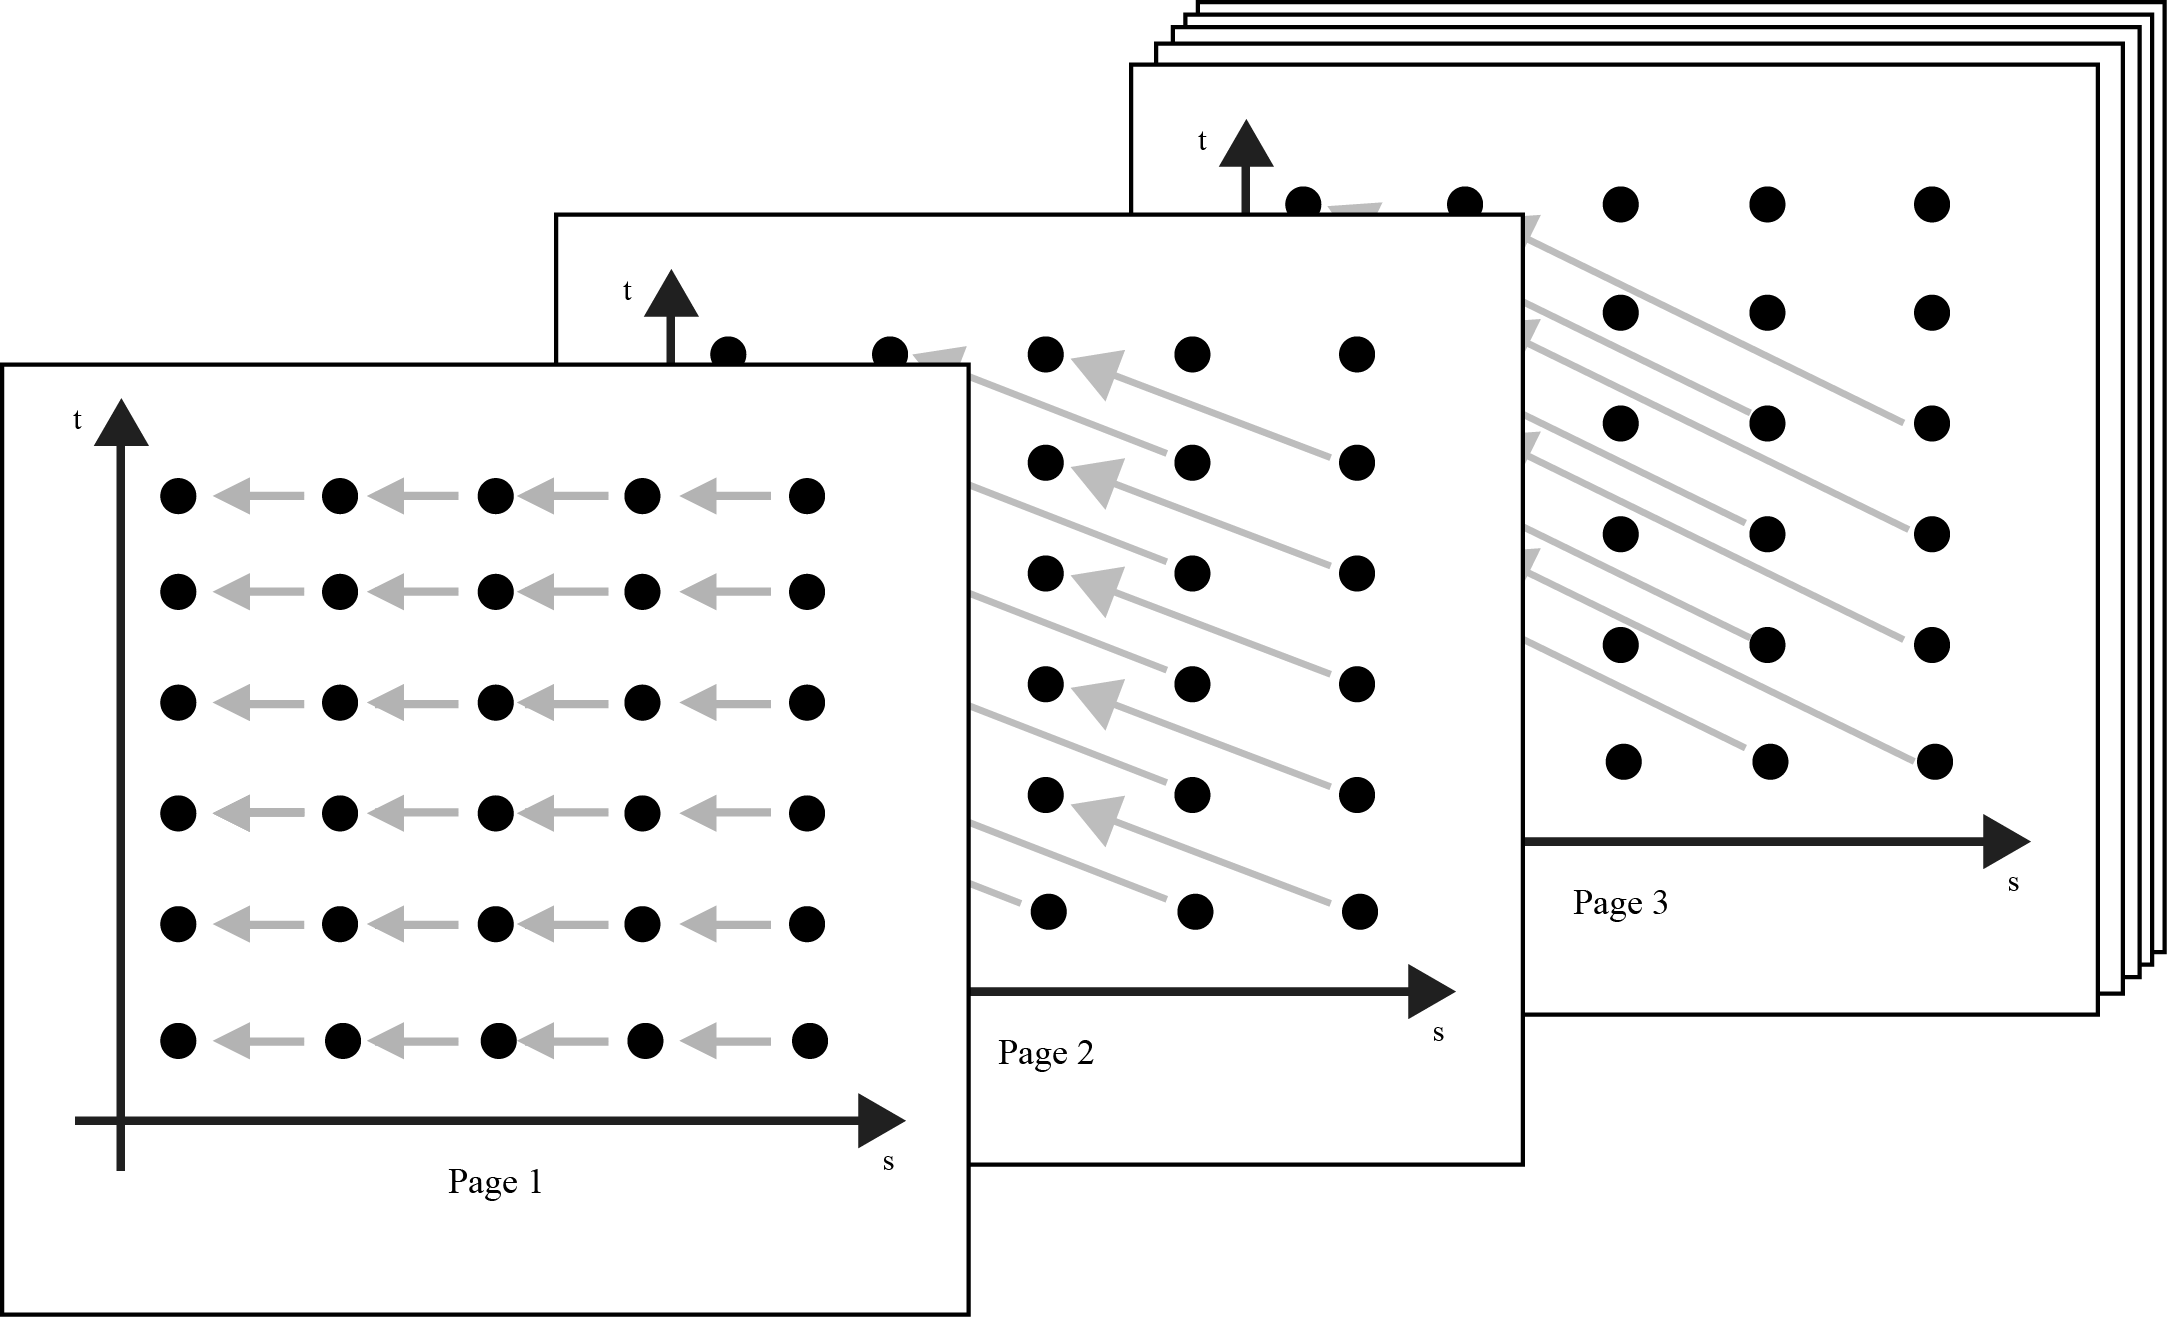
\includegraphics[width=\linewidth,height=0.5\textheight,keepaspectratio]{figures/cover.png}
  \end{center}
       \begin{minipage}{.35\linewidth}
    \begin{flushleft}
      \vspace{2em}
      {\fontsize{6pt}{2pt} \textit{Notes: These are notes live-tex'd
from a graduate course in Algebraic Curves taught by Pete Clark at the
University of Georgia in Fall 2020. As such, any errors or inaccuracies
are almost certainly my own. } } \\
    \end{flushleft}
    \end{minipage}
    \hfill
    \begin{minipage}{.65\linewidth}
    \end{minipage}
  }







\begin{document}

\date{}
\author{D. Zack Garza}
\maketitle
\begin{flushleft}
\textit{D. Zack Garza} \\
\textit{University of Georgia} \\
  \textit{\href{mailto: dzackgarza@gmail.com}{dzackgarza@gmail.com}} \\
{\tiny \textit{Last updated:} 2020-11-30 }
\end{flushleft}


\newpage

\tableofcontents
\newpage

\hypertarget{lecture-1-field-theory-preliminaries}{%
\section{Lecture 1: Field Theory
Preliminaries}\label{lecture-1-field-theory-preliminaries}}

\hypertarget{finite-generation-of-fields}{%
\subsection{Finite Generation of
Fields}\label{finite-generation-of-fields}}

See Chapter 11 of Field Theory notes.

\hypertarget{notion-1}{%
\subsubsection{Notion 1}\label{notion-1}}

\begin{definition}[Finitely Generated Field Extension]

A field extension \(\ell/k\) is \emph{finitely generated} if there
exists a finite set \(x_1, \cdots, x_n \in \ell\) such that
\(\ell = k(x_1, \cdots, x_n)\) and \(\ell\) is the smallest field
extension of \(k\).

Concretely, every element of \(\ell\) is a quotient of the form
\({p(x_1, \cdots, x_n) \over q(x_1, \cdots, x_n)}\) with
\(p, q\in k[x_1, \cdots, x_n]\).

\end{definition}

There are three different notions of finite generation for fields, the
above is the weakest.

\hypertarget{notion-2}{%
\subsubsection{Notion 2}\label{notion-2}}

The second is being finitely generated as an algebra:

\begin{definition}[Finitely Generated Algebras]

For \(R\subset S\) finitely generated algebras, \(S\) is finitely
generated over \(R\) if every element of \(S\) is a polynomial in
\(x_1, \cdots, x_n\), with coefficients in \(R\),
i.e.~\(S = R[x_1, \cdots, x_n]\).

\end{definition}

Note that this implies the previous definition, since anything that is a
polynomial is also a quotient of polynomials.

\hypertarget{notion-3}{%
\subsubsection{Notion 3}\label{notion-3}}

The final notion: \(\ell/k\) is finite (finite degree) if \(\ell\) is
finitely generated as a \(k\dash\)module, i.e.~a finite-dimensional
\(k\dash\)vector space.

\begin{definition}[Rational Function Field]

A \emph{rational function field} is
\(k(t_1, \cdots, t_n) \da ff \qty{ k[t_1, \cdots, t_n]}\).

\end{definition}

Note that we can make a similar definition for infinitely many
generators by taking a direct limit (here: union), and in fact every
element will only involve finitely many generators.

\begin{exercise}

\envlist

\begin{enumerate}
\def\labelenumi{\alph{enumi}.}
\item
  Show \(k(t) / k\) is finitely generated by notion (3) but not by (2).
\item
  Show that \(k[t]/k\) is (2) but not (1).\footnote{Note \(k[t]\) is not
    a field.}
\item
  Show that it is not possible for a \textbf{field} extension to satisfy
  (2) but not (1).\footnote{Hint: Zariski's lemma.}
\item
  Show that if \(\ell/k\) is finitely generated by (3) and algebraic,
  then it satisfies (1).
\end{enumerate}

\end{exercise}

\begin{theorem}[Field Theory Notes 11.19]

If \(L/K/F\) are field extensions, then \(L/F\) is finitely generated
\(\iff\) \(K/F\) and \(L/K\) are finitely generated.\footnote{See
  Artin-Tate Lemma, this doesn't necessarily hold for general rings.}

\end{theorem}

\begin{definition}[Algebraically Independent]

For \(\ell/k\), a subset \(\ts{x_i}\subset \ell\) is \emph{algebraically
independent} over \(k\) if no finite subset satisfies a nonzero
polynomial with \(k\) coefficients.

In this case, \(k[\ts{x_i}] / k\) is \emph{purely transcendental} as a
rational function field.

\end{definition}

\begin{theorem}[Existence of transcendence bases]

For \(\ell/k\) a field extension,

\begin{enumerate}
\def\labelenumi{\alph{enumi}.}
\item
  There exists a subset \(\ts{x_i}\subset \ell\) algebraically
  independent over \(k\) such that \(\ell/k(\ts{x_i})\) is algebraic.
\item
  If \(\ts{y_t}\) is another set of algebraically independent elements
  such that \(\ell/k(\ts{y_t})\) is algebraic, then
  \(\abs{\ts{x_i}} = \abs{\ts{y_t}}\).
\end{enumerate}

\end{theorem}

Thus every field extension is algebraic over a purely transcendental
extension. A subset as above is called a \emph{transcendence basis}, and
every 2 such bases have the same cardinality.

We have a notion of generation (similar to ``spanning''), independence,
and bases, so there are analogies to linear algebra (e.g.~every vector
space has a basis, any two have the same cardinality).\footnote{There is
  a common generalization: matroids.}

The following notion will be analagous to that of dimension in linear
algebra:

\begin{definition}[Transcendence Degree]

The \emph{transcendence degree} of \(\ell/k\) is the cardinality of any
transcendence basis.

\end{definition}

\begin{theorem}[Transcendence Degree is Additive in Towers]

If \(L/K/F\) are fields then
\(\trdeg(L/F) = \trdeg(K/F) + \trdeg(L/K)\).

\end{theorem}

\begin{theorem}[Bounds on Transcendence Degree]

Let \(K/k\) be finitely degenerated, so \(K = k(x_1, \cdots, x_n)\).
Then \(\trdeg(K/k) \leq n\), with equality iff \(K/k\) is purely
transcendental.

\end{theorem}

\begin{proof}

Suppose \(K\) is monogenic, i.e.~generated by one element. Then
\(\trdeg(F(x)/F) = \indic{x/F\text{ is transcendental}}\).

So the degree increases when a transcendental element is added, and
doesn't change when \(x\) is algebraic.

By additivity in towers, we take
\(k \injects k(x_1) \injects k(x_1, x_2) \injects \cdots \injects k(x_1, \cdots, x)n) = K\)
to obtain a chain of length \(n\). The transcendence degree is thus the
number of indices \(i\) such that \(x_i\) is transcendental over
\(k(x_1, \cdots, x_{i-1})\).\footnote{This is similar to checking if a
  vector is in the span of a collection of previous vectors.}

\end{proof}

\begin{definition}[Function fields in $d$ variables]

For \(d\in\ZZ^{\geq 0}\), an extension \(K/k\) is \emph{a function field
in \(d\) variables} (i.e.~of dimension \(d\)) if \(K/k\) is finitely
generated of transcendence degree \(d\).

\end{definition}

\begin{remark}

The study of such fields is birational geometry over the ground field
\(k\). \(k=\CC\) is of modern interest, things get more difficult in
other fields. The case of \(d=1\) is much easier: the function field
will itself be the geometric object and everything will built from that.
Our main tool will be \textbf{valuation theory}, where valuations will
correspond to points on the curve.

\end{remark}

\hypertarget{case-study-the-luxfcroth-problem.}{%
\subsection{Case Study: The Lüroth
Problem.}\label{case-study-the-luxfcroth-problem.}}

\begin{question}

For which fields \(k\) and \(d\in \ZZ^{\geq 0}\) is it true that if
\(k \subset \ell \subset k(t_1, \cdots, t_d)\) with
\(k(t_1 ,\cdots, t_d)/\ell\) finite then \(\ell\) is purely
transcendental?

\end{question}

\begin{answer}

It's complicated, and depends on \(d\) and \(k\). We have the following
partial results.

\end{answer}

\begin{theorem}[Lüroth]

True for \(d=1\): For any \(k\subset \ell \subset k(t)\),
\(\ell = k(x)\).

\end{theorem}

\begin{theorem}[Castelnuovo]

Also true for \(d=2, k=\CC\).

\end{theorem}

\begin{theorem}[Zariski]

No if \(d= 2\), \(k=\bar k\), and \(k\) is positive characteristic. Also
no if \(d=2, k\neq \bar k\) in characteristic zero.

\end{theorem}

\begin{theorem}[Clemens-Griffiths]

No if \(d\geq 3\) and \(k= \CC\).

\end{theorem}

\begin{remark}

Note that unirational need not imply rational for varieties.

\end{remark}

\begin{exercise}

Let \(k\) be a field, \(G\) a finite group with \(G\injects S_n\) the
Cayley embedding. Then \(S_n\) acts by permutation of variables on
\(k(t_1, \cdots, t_n)\), thus so does \(G\). Set
\(\ell \da k(t_1, \cdots, t_n)^G\) the fixed field, then by Artin's
observation in Galois theory: if you have a finite field acting
effectively by automorphisms on a field then taking the fixed field
yields a galois extension with automorphism group \(G\).

So \(\aut(k(t_1, \cdots, t_n)/ \ell) = G\).A

\begin{enumerate}
\def\labelenumi{\alph{enumi}.}
\tightlist
\item
  Suppose \(k=\QQ\), and show that an affirmative answer to the Lüroth
  problem implies an affirmative answer to the inverse galois problem
  for \(\QQ\).
\end{enumerate}

\begin{quote}
Hint: works for any field for which Hilbert's Irreducibility Theorem
holds.
\end{quote}

\begin{enumerate}
\def\labelenumi{\alph{enumi}.}
\setcounter{enumi}{1}
\item
  \(\ell /\QQ\) need not be a rational function field, explore the
  literature on this: first example due to Swan with \(\abs{G} = 47\).
\item
  Can still give many positive examples using the Shepherd-Todd Theorem.
\end{enumerate}

\end{exercise}

\todo[inline]{What's a global field?}

\hypertarget{integrals-closures-and-constant-fields}{%
\subsection{Integrals Closures and Constant
Fields}\label{integrals-closures-and-constant-fields}}

\begin{definition}[Integral Closure and Field of Constants]

For \(K/k\) a field extension, set \(\kappa(K)\) to be the algebraic
closure of \(k\) in \(K\), i.e.~special case of \emph{integral closure}.
If \(K/k\) is finitely generated, then \(\kappa(K)/k\) is finite degree.

Here \(\kappa(K)\) is called the \emph{field of constants}, and \(K\) is
also a function field over \(\kappa(K)\).

\end{definition}

\begin{remark}

In practice, we don't want \(\kappa(K)\) to be a proper extension of
\(k\). If this isn't the case, we replace considering \(K/k\) by
\(K/\kappa(K)\). If \(K/k\) is finitely generated, then

\begin{center}\begin{tikzcd}
k \arrow[rr, "\text{finite}", hook] &  & \kappa(K) \arrow[rr, "\text{finitely generated}", hook] &  & K
\end{tikzcd}\end{center}

Where we use the fact that from above, \(\kappa(K)/k\) is finitely
generated and algebraic and thus finite, and by a previous theorem, if
\(K/k\) is transcendental then \(K/\kappa(K)\) is as well, and thus
finitely generated. Thus if you have a function field over \(k\), you
can replace \(k\) by \(\kappa(K)\) and regard \(K\) as a function field
over \(\kappa(K)\) instead.

\end{remark}

\hypertarget{lecture-1-discussion-and-review}{%
\section{Lecture 1: Discussion and
Review}\label{lecture-1-discussion-and-review}}

\hypertarget{valuations}{%
\subsection{Valuations}\label{valuations}}

\begin{itemize}
\tightlist
\item
  Transcendence bases
\item
  Lüroth problem
\end{itemize}

For \(K/k\) a one variable function field, if we want a curve \(C/k\),
what are the points? We'll use \emph{valuations}, see NT 2.1. See also
completions, residue fields. If \(R \subset K\) a field, \(R\) is a
\emph{valuation ring} of \(K\) if for all \(x\in K\units\), at least one
of \(x, x^{-1} \in R\).

\begin{example}

The valuation rings of \(\QQ\) are
\(\ZZ_{(p)}\da \ZZ[\ts{{1\over \ell} \st \ell\neq p}]\) for all primes
\(p\).

\end{example}

See also \emph{Krull valuations}, which take values in some totally
ordered commutative group.

\begin{exercise}

Show that a valuation ring is a local ring, i.e.~it has a unique maximal
ideal.

\end{exercise}

\begin{example}

Where does the log come from?

There is a \(p\dash\)adic valuation:
\begin{align*}  
v: \QQ &\to \ZZ_{(p)} \\
{a\over b} = p^n {u \over v} &\mapsto n
.\end{align*}

Then we recover
\begin{align*}  
\ZZ_{(p)} = \ts {x\in \QQ\units \st v_p(x) \geq 0} \union \ts{0} \\
\mfm_{(p)} = \ts {x\in \QQ\units \st v_p(x) > 0} \union \ts{0} \\
.\end{align*}

There is a \(p\dash\)adic norm
\begin{align*}  
\abs{\wait}_p: \QQ &\to \RR \\
0 & \mapsto 0 \\
x &\mapsto p^{-n} = p^{-v_p(x)}
.\end{align*}

Then we get an ultrametric function, a non-archimedean function
\begin{align*}  
d_p: \QQ^2 \to \RR \\
(x, y) &\mapsto \abs{x- y}_p
.\end{align*}

We then recover \(v_p(x) = -\log_p \abs{x}_p\).\footnote{See NT 1 notes
  for more details on valuations.}

\end{example}

\hypertarget{places}{%
\subsection{Places}\label{places}}

For \(A\subset K\) a subring of a field, we'll be interested in the
place
\(\tilde \Sigma = \ts{\text{Valuation rings } R_v \text{ of } K} \st A \subset R_v \subsetneq K\).
Thus the valuation takes non-negative values on all elements of \(K\).
Can equip this with a topology (the ``Zariski'' topology, not the usual
one). This is always quasicompact, and called the \emph{Zariski-Riemann
space}. Can determine a sheaf of rings to make this a locally ringed
space.

We can define an equivalence of valuations and define the set of
\emph{places}
\begin{align*}  
\Sigma(K/k) \da \ts{\text{Nontrivial valuations } v\in K \st v(x) \geq 0\, \forall x\in k\units}
,\end{align*} which will be the points on the curve. Here the Zariski
topology will be the cofinite topology (which is not Hausdorff).
Scheme-theoretically, this is exactly the set of closed points on the
curve.

\begin{definition}[Generic Points]

A point \(p\in X\) a topological space is a \textbf{generic point} iff
its closure in \(X\) is all of \(X\).

\end{definition}

\begin{remark}

Note we will have unique models for curves, but this won't be the case
for surfaces: blowing up a point will yield a birational but
inequivalent surface.

\end{remark}

\hypertarget{divisors}{%
\subsection{Divisors}\label{divisors}}

\begin{definition}[Divisor Group]

The \emph{divisor group} of \(K\) is the free \(\ZZ\dash\)module on
\(\Sigma(K/k)\)

\end{definition}

\begin{remark}

This comes with a degree map
\begin{align*}  
\deg: \Div(K) \to \ZZ
\end{align*} which need not be surjective.

\end{remark}

\begin{definition}[Principal Divisors]

Consider the map
\begin{align*}  
\phi_d: K\units &\to \Div(K) \\
f &\mapsto (f)
.\end{align*} Then we define \(\im \phi_d\) as the subgroup of
\textbf{principal divisors}.

\end{definition}

\begin{definition}[Class Group]

Define the \textbf{class group} of \(K\) as
\begin{align*}  
\cl(K) \da \ts{\text{Divisors}} / \ts{\text{Principal divisors}} \da \Div(K) / \im \phi_d
.\end{align*}

\end{definition}

We can define the \textbf{class group} as divisors modulo principle
divisors \(\cl(K) = \Div(K) / \im(K\units)\) and the Riemann-Roch space
\(\mathcal{L}(D)\). The Riemann-Roch theorem will then be a statement
about \(\dim \mathcal{L}(D)\).

\hypertarget{lecture-2-field-theory-preliminaries}{%
\section{Lecture 2: Field Theory
Preliminaries}\label{lecture-2-field-theory-preliminaries}}

\hypertarget{base-extension}{%
\subsection{Base Extension}\label{base-extension}}

Given some object \(A/k\) and \(k\injects \ell\) is a field extension,
we would like some extended object \(A/\ell\).

\begin{example}

An \emph{affine variety} \(V/k\) is given by finitely many polynomials
in \(p_i \in k[t_1, \cdots, t_n]\), and base extension comes from the
map \(k[t_1, \cdots, t_n] \injects \ell[t_1, \cdots, t_n]\). More
algebraically, we have the affine coordinate ring over \(k\) given by
\(k[V] = k[t_1,\cdots, t_n]/\gens{p_i}\), the ring of polynomial
functions on the zero locus corresponding to this variety. We can
similarly replace \(k\) be \(\ell\) in this definition. Here we can
observe that \(\ell[V] \cong k[V] \tensor_k \ell\).

\end{example}

In general we have a map
\begin{align*}  
\wait \tensor_k \ell & \\
\ts{k\dash\text{vector spaces}} &\to \ts{\ell\dash\text{vector spaces}} \\
\ts{k\dash\text{algebras}} &\to\ts{\ell\dash\text{algebras}}
.\end{align*} This will be an exact functor on the category
\(k\dash\text{Vect}\), i.e.~\(\ell\) is a flat module. Here everything
is free, and free \(\implies\) flat, so things work out nicely.

What about for function fields? Since \(k\) is a \(k\dash\)algebra, we
can consider \(k\tensor_k \ell\), however this need not be a field. Note
that tensor products of fields come up very often, but don't seem to be
explicitly covered in classes! We will broach this subject here.

\begin{exercise}

If \(\ell/k\) is algebraic and \(\ell\tensor_k \ell\) is a domain, the
\(\ell = k\).

\end{exercise}

\begin{remark}

In other words, this is rarely a domain. A hint: start with the
monogenic case, and also reduce to the case where the extension is not
just algebraic but finite.

\end{remark}

\begin{remark}

Tensor products of field extensions are still interesting: if \(\ell/k\)
is finite, it is galois \(\iff\)
\(\ell \tensor_k \ell \cong \ell^{[\ell: k]}\). So its dimension as an
\(\ell\dash\)algebra is equal to the degree of \(\ell/k\), so it splits
as a product of copies of \(\ell\).

We'd like the tensor product of a field to be a field, or at least a
domain where we can take the fraction field and get a field. This hints
that we should not be tensoring algebraic extensions, but rather
transcendental ones.

\end{remark}

\begin{exercise}

For \(\ell/k\) a field extension,

\begin{enumerate}
\def\labelenumi{\alph{enumi}.}
\item
  Show \(k(t) \tensor_k \ell\) is a domain with fraction field
  \(\ell(t)\).
\item
  Show it is a field \(\iff\) \(\ell/k\) is algebraic.
\end{enumerate}

\end{exercise}

\begin{proposition}[FT 12.7, 12.8]

Let \(k_1, k_2 / k\) are field extensions, and suppose
\(k_1 \tensor_k k_2\) is a domain. Then this is a field \(\iff\) at
least one of \(k_1/k\) or \(k_2/k\) is algebraic.\footnote{Reminder: for
  \(\ell/k\) and \(\alpha\in \ell\) algebraic over \(k\), then
  \(k(\alpha) = k[\alpha]\).}

\end{proposition}

So we'll concentrate on when \(K \tensor_k \ell\) is a domain.

\hypertarget{when-extensions-preserve-being-a-domain}{%
\subsection{When Extensions Preserve Being a
Domain}\label{when-extensions-preserve-being-a-domain}}

\begin{question}

What's the condition on a function field \(K/k\) that guarantees this,
i.e.~when extending scalars from \(k\) to \(\ell\) still yields a
domain?

\end{question}

\begin{definition}[Base Change]

If this remains a domain, we'll take the fraction field and call it the
\textbf{base change}.

\end{definition}

\begin{exercise}

If \(K/k\) is finitely generated (i.e.~a function field) and
\(K\tensor_k \ell\) is a domain, then \(ff(K\tensor_k \ell)/\ell\) is
finitely generated.

\end{exercise}

\begin{remark}

The point here is that if taking a function field and extending scalars
still results in a domain, we'll call the result a function field as
well. Most of all, we want to base change to the algebraic closure.
We'll have issues if the constant field is not just \(k\) itself:

\end{remark}

\begin{lemma}

If \(K\tensor_k \bar k\) is a domain, then the constant field
\(\kappa(K) = k\).

\end{lemma}

\begin{proof}

Use the fact that \(\wait \tensor_k V\) is exact. We then get an
injection

\begin{center}\begin{tikzcd}
\kappa(K) \tensor_k \kappa(K) \ar[rr, hookrightarrow]\ar[rd, hookrightarrow] & &
K \tensor_k \bar k \\
& \kappa(K) \tensor_k \bar k\ar[ru, hookrightarrow] & 
\end{tikzcd}\end{center}

Here we use the injections \(\kappa(K) \injects \bar k\) and
\(\kappa(K) \injects K\).

We now have an injection of \(k\dash\)algebras, and subrings of domains
are domains. So apply the first exercise: the only way this can happen
is if \(\kappa(K) = k\).

\end{proof}

\begin{exercise}[the simplest possible case]

Describe \(\CC(t) \tensor_\RR \CC\), tensored as \(\RR\dash\)algebras.

\end{exercise}

\begin{remark}

Won't be a domain by the lemma, and will instead be some
\(\CC(t)\dash\)algebra of dimension 2.

\end{remark}

\hypertarget{good-base-change-for-function-fields}{%
\subsection{Good Base Change For Function
Fields}\label{good-base-change-for-function-fields}}

In order to have a good base change for our function fields, we want to
constant extension to be trivial, i.e.~\(\kappa(K) = k\). This requires
that the ground field be algebraically closed.

In this case, you might expect that extending scalars to the algebraic
closure would yield a field again. This is true in characteristic zero,
but false in positive characteristic.

\begin{question}[a more precise one]

If \(\kappa(K) = k\), must \(K\tensor_K \bar k\) be a field?

\end{question}

If that's true and we're in positive characteristic, recalling the for
an algebraic extension this being a field is equivalent to it being a
domain. But if that's a domain, the tensor product of every algebraic
extension must be a domain, which is why this is an important case.

If so, then \(K\tensor_k k^{1\over p}\) is a field, where
\(k^{1\over p} \da k\qty{\ts{x^{1\over p} \st x\in k }}\) is obtained by
adjoining all \(p\)th roots of all elements. This is a purely
inseparable extension. The latter condition (this tensor product being a
field) is one of several equivalent conditions for a field to be
separable.\footnote{Note that the frobenius maps
  \(k^{1\over p} \surjects k\), so this is sort of like inverting this
  map.}

\begin{remark}

Recall that \(K/k\) is transcendental, and there is an extended notion
of separability for non-algebraic extensions. Another equivalent
condition is that every finitely generated subextension is separably
generated, i.e.~it admits a transcendence basis \(\ts{x_i}\) such that
\(k\injects k(\ts{x_i}) \injects F\) where \(F/k(\ts{x_i})\) is
algebraic and separable. Such a transcendence basis is called a
\emph{separating transcendence basis}. Since we're only looking at
finitely generated extensions, we wont' have to worry much about the
difference between separable and separably generated.

\end{remark}

\begin{question}

What's the point? There's an extra technical condition to ensure the
base change is a field: the function field being separable over the
ground field. Is this necessarily the case if \(\kappa(K) = k\)?

\end{question}

\begin{answer}

No, for fairly technical reasons. \lmargnote{\danger}

\end{answer}

\begin{example}

\label{technical_example} Set \(k = \FF_p(a, b)\) a rational function
field in two variables as the ground field. Set
\begin{align*}  
A \da k[x, y]/ \gens{ax^p + b-y^b}
.\end{align*} Then \(A\) is a domain, so set \(k = ff(A)\).

\begin{claim}

\(\kappa(K) = k\), so \(k\) is algebraically closed in this extension,
but \(K/k\) is \emph{not} separable.

\end{claim}

How to show: extending scalars to \(k^{1\over p}\) does not yield a
domain.

Let \(\alpha, \beta \in \bar k\) such that
\(\alpha^p = a, \beta^b = b\), so
\begin{align*}  
ax^p + b-y^b = (\alpha x + \beta - y)^p
,\end{align*} which implies \(K \tensor_k k^{1\over p}\) is not a
domain: \(k[x, y]\) is a UFD, so the quotient of a polynomial is a
domain iff the polynomial is irreducible. However, the \(p\)th power map
is a homomorphism, and this exhibits the image of the defining
polynomial as something non-irreducible.

\end{example}

\begin{remark}

Note that \(f(x, y) = ax^p + b - y^p\) is the curve in this situation.
The one variable function field is defined by quotienting out a function
in two variables and taking the function field. Every 1-variable
function field can be obtained in this way. Therefore this polynomial is
irreducible, but becomes reducible over the algebraic closure. So we'd
like the polynomial to be irreducible over both.

\end{remark}

\begin{remark}

This is pretty technical, but we won't have to worry if
\(k = k^{1\over p}\). Equivalently, frobenius is surjective on \(k\),
i.e.~\(k\) is a perfect field.

If \(k\) is not perfect, it can happen (famous paper of Tate) making an
inseparable base extension can decrease the genus of the curve.

\end{remark}

Recall that the perfect fields are given by:

\begin{itemize}
\tightlist
\item
  Anything characteristic zero, every reducible polynomial is separable.
\item
  Any algebraically closed field
\item
  Finite fields (frobenius is always injective)
\end{itemize}

Imperfect fields include:

\begin{itemize}
\tightlist
\item
  Function fields in characteristic \(p\)
\item
  Complete discretely valued fields \(k((t))\) in characteristic \(p\)
  \footnote{This is a good time to review valuations and uniformizing
    elements from NTII.}
\end{itemize}

\begin{theorem}[FT 12.20: Regular Field Extensions]

For field extensions \(K/k\), TFAE

\begin{enumerate}
\def\labelenumi{\arabic{enumi}.}
\item
  \(\kappa(K) = k\) and \(K/k\) is separable
\item
  \(K\tensor_k \bar k\) is a domain, or equivalently a field
\item
  For all field extensions \(\ell/k\), \(K\tensor_k \ell\) is a domain.
\end{enumerate}

\end{theorem}

\begin{remark}

Note that this allows making not just an algebraic base change, but a
totally arbitrary one.

\end{remark}

\begin{definition}[?]

A field extension satisfying these conditions is called
\textbf{regular}.

\end{definition}

\begin{remark}

Regular corresponds to ``nonsingular'' in this neck of the woods. The
implication \(2\implies 3\) is the interesting one. To prove it, reduces
to showing that if \(k= \bar k\) and \(R_i\) are domains that are
finitely generated as \(k\dash\)algebras, then \(R_1 \tensor_k R_2\) is
also a domain. This doesn't always happen,
e.g.~\(\QQ(\sqrt{2}) \tensor_\QQ \QQ(\sqrt{2})\) is not a domain. Really
need algebraically closed.

This is a result in affine algebraic geometry. An algebra that is a
domain and finitely generated over a field is an \emph{affine algebraic
variety}, more precisely it is integral. The tensor product on the
coordinate ring side corresponds to taking the product of varieties.
Thus the fact here is that a product of integral varieties remains
integral, as long as you're over an algebraically closed field. Proof
uses Hilbert's Nullstellensatz.

\end{remark}

\begin{exercise}

\envlist

\begin{enumerate}
\def\labelenumi{\alph{enumi}.}
\item
  Show that \(k(t) / k\) is regular. \footnote{I.e.
    \(k(t)\tensor_k \bar k\) is a domain.}
\item
  Show every purely transcendental extension is regular.
\item
  Show that for a field \(k\), every extension is regular \(\iff\)
  \(k = \bar k\).
\item
  Show \(K/k\) is regular \(\iff\) every finitely generated subextension
  is regular.
\end{enumerate}

\end{exercise}

\hypertarget{example-of-a-non-regular-family-of-function-fields}{%
\subsection{Example of a Non-Regular Family of Function
Fields}\label{example-of-a-non-regular-family-of-function-fields}}

Choose an elliptic curve \(E/\QQ(t)\) with \(j\dash\)invariant \(t\).
For \(N\in \ZZ^{+}\), define \(\tilde K_N \da \QQ(t)(E[N])\) the
\(N\dash\)torsion field of \(E\). Then \(\tilde K_N/\QQ(t)\) is a finite
galois extension with galois group isomorphic to the image of the
modular galois representation \footnote{See Cornell-Silverman-Stevens
  covering the proof of FLT, modular curves from the function field
  perspective.}

\begin{align*}  
\rho_N: g(\QQ(t)) \to \GL(2, \ZZ/N\ZZ) \mod N
.\end{align*}

\begin{proposition}[Some Facts]

\(\rho_N\) is surjective, and
\begin{align*}  
\Aut(\tilde K_N / \QQ(t))  \cong \GL(2, \ZZ/N\ZZ)
.\end{align*}

\(\det \rho_N = \chi_N \mod N\), the cyclotomic character, and therefore
\(\chi_N\) restricted to \(g(\tilde K_N)\) is trivial, so
\(\tilde K_N \supset \QQ(\zeta_N)\). For \(N\geq 3\),
\(\QQ(\zeta_N) \supsetneq \QQ\), so \(\tilde K_N / \QQ(t)\) is a
non-regular function field.

\end{proposition}

\begin{remark}

Actually \(\tilde K_N\) depends on the choice of \(E\): difference
choices of nonisomorphic curves with the same \(j\dash\)invariant differ
by a quadratic twist and the \(\rho_N\) differ by a quadratic character
on \(g(\QQ(t))\). Importantly, this changes the kernel, and thus the
field.

\end{remark}

To fix this, we look at the \emph{reduced galois representation}, the
following composition:
\begin{align*}  
\bar \rho_N: g(\QQ(t)) \to \GL(2, \ZZ/N\ZZ) \surjects \GL(2, \ZZ/N\ZZ)/\ts{\pm I}
.\end{align*}

We obtain a field theory diagram

\begin{center}
\begin{tikzcd}
\ar[dd, bend right, "{\GL(2, \ZZ/N\ZZ)}"'] \bar K_N \ar[d, bend left, "\ts{\pm I}"] &\\
K_N \ar[d, bend left, "{\GL(2, \ZZ/N\ZZ)/\ts{\pm I}}"] &\\
\QQ(t)&
\end{tikzcd}
\end{center}

So if you just take the field fixed by \(\pm I\), you get \(K_N\). In
this case, the reduced galois representation depends only on the
\(j\dash\)invariant, and not on the model chosen. So the function field
\(K_N/\QQ(t)\) is the ``canonical'' choice.

\begin{question}

Does this make \(K_N/\QQ(t)\) regular?

\end{question}

\begin{answer}

No, \(\rho_N(g(K_N)) = \ts{\pm I}\) and \(\det(\pm I) = 1\), so we still
have \(K_N \supset \QQ(\zeta_N)\).

\end{answer}

In this course, we'll identify algebraic curves over \(k\) and
one-variable function fields \(K/k\). The function field \(K_N\)
corresponds to an algebraic curve \(X(N)/\QQ\) that is ``nicer'' over
\(\QQ(\zeta_N)\). In fact, see Rohrlich: \(\kappa(K_N) = \QQ(\zeta_N)\).
Our curves will have points (equal to valuations) which will have
degrees. If the constant subfield is not just \(k\), this prevents
degree 1 points on the curve. By Galois theory, for every subgroup
\(H \subseteq \GL(2, \ZZ/N\ZZ) / \ts{\pm I}\), we'll get a function
field \(\QQ(H) \da H_N^H\).gg In this case, \(\QQ(H)/\QQ\) is regular
\(\iff\) \(\det(H) = (\ZZ/N\ZZ)\units\).

Later we'll understand the residues at points as the residue fields of
some DVRs, then the residue field will always contain the field of
constants.

\hypertarget{lecture-3-last-of-preliminaries}{%
\section{Lecture 3: Last of
Preliminaries}\label{lecture-3-last-of-preliminaries}}

Today we'll be wrapping up the last of the preliminaries. Upcoming:
one-variable function fields and their valuation rings.

\hypertarget{polynomials-defining-regular-function-fields}{%
\subsection{Polynomials Defining Regular Function
Fields}\label{polynomials-defining-regular-function-fields}}

\begin{question}

Where's the curve in all of this?

\end{question}

\begin{answer}

This will come from an equation like \(f(x, y) = 0\).

\end{answer}

\begin{exercise}

Let \(R_1, R_2\) be \(k\dash\)algebras that are also domains with
fraction fields \(K_i\). Show \(R_1 \tensor_k R_2\) is a domain \(\iff\)
\(K_1 \tensor_k K_2\) is a domain.\footnote{Hint: use a denominator
  clearing argument.}

\end{exercise}

\hypertarget{geometric-irreducibility}{%
\subsection{Geometric Irreducibility}\label{geometric-irreducibility}}

\begin{definition}[Geometrically Irreducible Polynomial]

A polynomial of positive degree \(f\in k[t_1, \cdots, t_n]\) is
\textbf{geometrically irreducible} if \(f\in \bar k[t_1, \cdots, t_n]\)
is irreducible as a polynomial.

\end{definition}

\begin{remark}

If \(n=1\) then \(f\) is geometrically irreducible \(\iff\) \(f\) is
linear, i.e.~of degree 1. Let \(f\) be irreducible, then since
polynomial rings are UFDs then \(\gens{f}\) is a prime ideal
(irreducibles generate principal ideals) and
\(k[t_1, \cdots, t_n]/\gens{f}\) is a domain. Let \(K_f\) be the
fraction field.

\end{remark}

\begin{exercise}[an easy one]

\envlist

\begin{enumerate}
\def\labelenumi{\alph{enumi}.}
\item
  Above for \(1\leq i \leq n\) let \(x_i\) be the image of \(t_i\) in
  \(K_f\). Show that \(K_f = k(x_1, \cdots, x_n)\).
\item
  Show that if \(K/k\) is generated by \(x_1, \cdots, x_n\), then it is
  the fraction field of \(k[t_1, \cdots, t_n] /\mfp\) for some prime
  ideal \(\mfp\) (equivalently, a height 1 ideal).
\end{enumerate}

\end{exercise}

\begin{proposition}[?]

Suppose that \(f\) is geometrically irreducible.

\begin{enumerate}
\def\labelenumi{\alph{enumi}.}
\item
  The function field \(K/k\) is regular.
\item
  For all \(\ell/k\), \(f\in \ell[t_1, \cdots, t_n]\) is irreducible.
\end{enumerate}

\end{proposition}

\begin{definition}[Absolutely Irreducible Polynomial]

In this case we say \(f\) is \textbf{absolutely irreducible} as a
synonym for geometrically irreducible.

\end{definition}

\begin{proof}

By definition of geometric irreducibility,
\(\bar k[t_1, \cdots, t_n]/\gens{f} = k[t_1, \cdots, t_n]/\gens{f} \tensor_k \bar k\)
is a domain. The exercise shows that \(K_f \tensor_k k\) is a domain, so
\(K_f\) is regular. It follows that for all \(\ell/k\),
\(K_f \tensor_k \ell\) is a domain, so
\(\ell[t_1, \cdots, t_n]/\gens{f}\) is a domain.

\end{proof}

\begin{slogan}

Geometrically irreducible polynomials are good sources of regular
function fields.

\end{slogan}

\begin{exercise}

Let \(k\) be a field, \(d\in \ZZ^+\) such that \(4\notdivides d\) and
\(p(x) \in k[x]\) be positive degree. Factor
\(p(x) = \prod_{i=1}^r (x-a_i)^{\ell_i}\) in \(\bar k[x]\).

\begin{enumerate}
\def\labelenumi{\alph{enumi}.}
\item
  Suppose that for some \(i\), \(d\notdivides \ell_i\). Show that
  \(f(x, y) \da y^d - p(x) \in k[x, y]\) is geometrically irreducible.
  Conclude that \(K_f \da ff\qty{k[x, y] / \gens{y^d - p(x)}}\) is a
  regular one-variable function field over \(k\), and thus elliptic
  curves yield regular function fields.\footnote{Referred to as
    \emph{hyperelliptic} or \emph{superelliptic} function fields. Hint:
    use FT 9.21 or Lang's Algebra.}
\item
  What happens when \(4\divides d\)?
\end{enumerate}

\end{exercise}

\begin{exercise}[Nice, Recommended]

Assume \(k\) is a field, if necessary assuming \(\ch(k) \neq 2\).

\begin{enumerate}
\def\labelenumi{\alph{enumi}.}
\item
  Let \(f(x, y) = x^2 - y^2 -1\) and show \(K_f\) is is rational:
  \(K_f = k(z)\).
\item
  Let \(f(x, y) = x^2 + y^2 - 1\). Show that \(K_f\) is again rational.
\item
  Let \(k = \CC\) and \(f(x, y) = x^2 + y^2 + 1\), \(K_f\) is rational.
\item
  Let \(k= \RR\). For \(f(x ,y) = x^2 + y^2 + 1\), is \(K_f\)
  rational?\footnote{This is an example of a non-rational genus zero
    function field.}
\end{enumerate}

\end{exercise}

\begin{question}

Can we always construct regular function fields using geometrically
irreducible polynomials?

\end{question}

\begin{answer}

In several variables, no, since not every variety is birational to a
hypersurface. In one variable, yes, as the following theorem shows:

\end{answer}

\hypertarget{our-function-fields-are-geometrically-irreducible}{%
\subsection{Our Function Fields are Geometrically
Irreducible}\label{our-function-fields-are-geometrically-irreducible}}

\begin{theorem}[Regular Function Fields in One Variable are Geometrically Irreducible]

Let \(K/k\) be a one variable function field (finitely generated,
transcendence degree one). Then

\begin{enumerate}
\def\labelenumi{\alph{enumi}.}
\item
  If \(K/k\) is separable, then \(K = k(x, y)\) for some \(x, y\in K\).
\item
  If \(K/k\) is regular (separable + constant subfield is \(k\), so
  stronger) then \(K \cong K_f\) for a geometrically irreducible
  \(f\in k[x ,y]\).
\end{enumerate}

\end{theorem}

Recall separable implies there exists a separating transcendence basis.

\begin{proof}[of a]

This means there exists a primitive element \(x\in K\) such that
\(K/k(x)\) is finite and separable. By the Primitive Element Corollary
(FT 7.2), there exist a \(y\in K\) such that \(K = k(x, y)\).

\end{proof}

\begin{proof}[of b]

Omitted for now, slightly technical.

\end{proof}

\begin{remark}

Importance of last result: a regular function field on one variable
corresponds to a nice geometrically irreducible polynomial \(f\).

\end{remark}

\begin{remark}

Note that the plane curve module may not be smooth, and in fact usually
is not possible. I.e. \(k[x ,y]/\gens{f}\) is a one-dimensional
noetherian domain, which need not be integrally closed.

\end{remark}

\begin{question}

Can every one variable function field be 2-generated?

\end{question}

\begin{answer}

Yes, as long as the ground field is perfect. In positive characteristic,
the suspicion is no: there exists finite inseparable extensions
\(\ell/k\) that need arbitrarily many generators. However, what if
\(K/k\) has constant field \(k\) but is not separable? Riemann-Roch may
have something to say about this.

\end{answer}

\begin{example}

\hyperref[technical_example]{Example from earlier lecture:}

\begin{align*}
ax^p + b - y^b
\end{align*}

\end{example}

\begin{remark}

We can find examples of nice function fields by taking irreducible
polynomials in two variables. This will define a one-variable function
field. If the polynomial is geometrical reducible, this produces regular
function fields.

\end{remark}

\hypertarget{lecture-4-chapter-1-one-variable-function-fields-and-their-valuations}{%
\section{Lecture 4 (Chapter 1: One Variable Function Fields and Their
Valuations)}\label{lecture-4-chapter-1-one-variable-function-fields-and-their-valuations}}

Since we have the field-theoretic preliminaries out of the way, we now
start studying one-variable function fields in earnest. The main
technique that we use to extract the geometry will be the theory of
valuations. These may be familiar from NTII, but we will cover them in
more generality here.

\hypertarget{valuation-rings-and-krull-valuations}{%
\subsection{Valuation Rings and Krull
Valuations}\label{valuation-rings-and-krull-valuations}}

Recall that NTII approach to valuations:

\begin{definition}[Valuation]

A \textbf{valuation} on a field \(K\) is a map
\(v:K\to \RR\union \ts\infty\) such that \(v(K\units) \subset \RR\),
\(v(0) = \infty\), and \(v\) is of the form \(-\log(\abs{\wait})\) where
\(\abs{\wait}: K \to [0, \infty)\) is an \emph{ultrametric
norm}.\footnote{In other words, \(e^{-v(\wait)}\) is an ultrametric
  norm.} Recall that an \emph{ultrametric norm} satisfies not only the
triangle inequality but the ultrametric triangle inequality,
i.e.~\(d(x, z) \leq \max(x, z)\).

\end{definition}

We now take an algebraic approach to this definition, where we'll end up
replacing \(\RR\) with something more general.

\begin{definition}[Valuation Ring]

A subring \(R\) of a field \(K\) is a \textbf{valuation ring} if for all
\(x\in K\units\), at least one of \(x\) or \(x^{-1}\) is in \(R\).

\end{definition}

\begin{remark}

This is a ``largeness'' property. It also implies that \(K = \ff(R)\).

\end{remark}

\hypertarget{group-of-divisibility}{%
\subsection{Group of Divisibility}\label{group-of-divisibility}}

\begin{definition}[Group of Divisibility]

Given any integral domain \(R\) with fraction field \(K\), the
\textbf{group of divisibility} \(G(R)\) is defined as the
\emph{partially ordered commutative group}\footnote{This means that the
  two structures are compatible.}

\begin{align*}  
G(R) \da K\units / R\units
.\end{align*} We will write the group law here additively. The ordering
is given by \(x\leq y \iff y/x \in R\).

\end{definition}

\begin{remark}

Note that the way the partial order is written, it's a relation on
\(K\units\), but it is not quite a partial ordering there. It is
reflexive and transitive, but need not be antireflexive: if
\(x/y, y/x\in R\) then \(x,y\) differ by an element of \(u\in R\units\)
so that \(x=uy\). In particular, they need not be equal. This gives a
structure of a \emph{quasiordering}, and if you set
\(x\sim y \iff x\leq y\) and \(y\leq x\), this leads to an equivalence
relation, and modding out by it yields a partial order. Here this is
accomplished by essentially trivializing units.\\

Another way to think of \(G(R)\) is as the nonzero principal fractional
ideals of \(K\), since any two generators of an ideal will differ by a
unit.

\end{remark}

\begin{remark}

Inside this group there is a \emph{positive cone} \(G(R)^+\) of elements
that are ``nonnegative'': since we're in a commutative setting, the zero
element is equal to 1, and the positive cone is given by
\(\ts{y\geq 0} = \ts{y\in R}\), and is thus given by the group
\(G(R)^+ = (R, \cdot)\).\\

This is very general: if you're studying factorization in integral
domains, many properties are reflected in \(G(R)\). E.g. being a UFD
(the most important factorization property!) implies that \(G(R)\) is a
free commutative group.

\end{remark}

\begin{remark}

In general this is only a \emph{partially} ordered group and not totally
ordered. For example, take \(R = \ZZ\) and \(x=2, y=3\), then neither of
\(2/3, 3/2\) are in \(\ZZ\), so \(x\not\leq y\) and \(y\not\leq x\). On
the other hand, if we do have a total order, then either \(x\) or
\(x^{-1}\) is in the ring, which are exactly valuation subring of a
field.

\end{remark}

\begin{claim}

\(R\) is a valuation ring \(\iff\) \(G(R)\) is totally ordered.

\end{claim}

\begin{remark}

Note that \(\RR\) is a totally ordered group.

\end{remark}

\hypertarget{generalized-valuations}{%
\subsection{Generalized Valuations}\label{generalized-valuations}}

This makes \(G(R)\) the ``target group'' of a generalized analytic
valuation. Whenever we have a valuation ring, we have a totally ordered
commutative group, and the valuation \(v: K\units \to G(R)\) is a
quotient map which we can extend to \(K\) by \(v(0) \da \infty\). This
has some familiar properties:

\begin{itemize}
\tightlist
\item
  (VRK1) For all \(x,y\in K\units\),\footnote{This follows from the fact
    that the quotient map is a group morphism. Note that the additive
    notation makes this more suggestive of what an original valuation
    satisfied.}
\end{itemize}

\begin{align*}  
v(xy) = v(x) + v(y)
.\end{align*}

\begin{itemize}
\tightlist
\item
  (VRK2) For all \(x,y \in K\units\) such that \(x+y\neq 0\),
  \begin{align*}  
  v(x+y) \geq \min(v(x), v(y))
  .\end{align*}
\end{itemize}

For ultrametric norms, all triangles are isosceles: is that true for
this type of function? The answer is yes, by the following exercise:

\begin{exercise}[?]

If \(v(x) \neq v(y)\), then \(v(x+y) = \min(v(x), v(y))\).

\end{exercise}

So the properties here are formally identical to the NTII notion of
valuation, with \((\RR, +, \leq)\) replaced by \((G(R), +, \leq)\).

\begin{exercise}[?]

Conversely, if \(v: K\units \to G\) is a map into a totally ordered
commutative group satisfying VRK1 and VRK2\footnote{Any such map
  satisfying these two properties is a \textbf{Krull valuation}, Krull's
  generalization of classical valuations.}, then
\begin{align*}  
R_v \da \ts {x\in K\units \st v(x) \geq 0} \union \ts{0}
\end{align*} is a valuation ring.\footnote{Note that in a totally
  ordered group, either \(v(x) \geq 0\) or \(-v(x) \geq 0\), so we get
  the property that either \(x, x^{-1} \in R_v\).} We can thus extract
valuation rings in this situation.

\end{exercise}

\begin{exercise}[?]

A valuation ring is \textbf{local}, i.e.~there is a unique maximal ideal
\begin{align*}  
\mathfrak{m}_v \da \ts{x\in K\units \st v(x) > 0} \union \ts{0}
.\end{align*}

\end{exercise}

\begin{remark}

These two constructions are morally mutually inverse. This doesn't hold
on the nose, since there is extraneous data in the new analytic
valuation. Recall that in NTII we have a notion of equivalence of norms,
and two distinct norms that are equivalent can give rise to the same
valuation. For example, given a valuation, one can scale it by
\(\alpha \in \RR\), and it's easy to check that this gives the same
valuation. It is possible for the valuation not to surject onto \(\RR\),
but this doesn't happen in practice. The image is usually infinite
cyclic, what we call a \emph{discrete valuation}, and so one is led to
the definition of the \emph{value group} of the valuation as its image.
If you have a notion of equivalence of Krull valuations, you want to
allow for isomorphisms of the value group. The cleanest notion of
equivalence is thus the following:

\end{remark}

\begin{definition}[Equivalence of Krull valuations]

Two Krull valuations on a field \(K\) are \textbf{equivalent} iff their
valuation rings are \emph{equal}.

\end{definition}

\begin{remark}

Going back to NTII, if you have two nonarchimedean norms on a field,
then there are many equivalent conditions for equivalence, and this is
one of them.

\end{remark}

Some general valuation theory:

\begin{itemize}
\item
  Every totally ordered commutative group is a group of
  divisibility.\footnote{Pete's Commutative Algebra Notes, Ch. 17.10}
\item
  A totally ordered group has \textbf{rank 1} if it is nontrivial and
  embeds into \(\RR\)

  \begin{itemize}
  \tightlist
  \item
    If the value group is trivial, \(R = K\)
  \end{itemize}
\item
  A Krull valuation of rank at most 1 is the NTII notion of a valuation.
\end{itemize}

\begin{exercise}[?]

For \(n\geq 2\), put the lexicographic order on \(\ZZ^n\), and show this
has rank strictly larger than 1. Thus \(\ZZ^n\injects \RR\) as a
commutative group, but not as a totally ordered commutative group.

\end{exercise}

\begin{remark}

In fact, for any ordered group \(G\), one can attach a rank: a cardinal
number \(r(G)\). Here, \(r((\ZZ^n, \text{lex})) = n\). This is useful
when studying \(\spec(R)\) for \(R\) a DVR.

\end{remark}

A valuation of rank bigger than 1 does not induce a norm on \(K\) in the
metric sense, although this is not so important. A closer notion is
expanding the notion of a metric space by allowing the metric to be
defined on \(X\) as \(d: X\cross X \to R\) for some \(R\) more general
than \(\RR\), like a totally ordered group or a nonarchimedean field.
This would yield a class of topological spaces that are reminiscent of
metric spaces.

\hypertarget{regular-or-centered-valuations}{%
\subsection{Regular or Centered
Valuations}\label{regular-or-centered-valuations}}

\begin{definition}[Important: Regular and Centered]

Let \(v:K\units \to (G, +)\) be a Krull valuation and let
\(A \subset K\) be a subring of \(K\). Then \(v\) is
\textbf{\(A\dash\)regular} or \textbf{centered in \(A\)} if \(A\) is a
subset of some valuation ring \(R_v\). In this case,
\(\mathfrak{p} \da \mathfrak{m}_v \intersect A \in \spec(A)\) is denoted
the \textbf{center of \(v\) in \(A\)}.\footnote{Here \(\mathfrak{m}_v\)
  denotes pulling back the maximal ideal along this morphism of rings.}

\end{definition}

\begin{remark}

The term regularity here arises because we'll want to think of elements
of \(A\) as functions and the valuation as a type of point, then the
notion of being a regular function at a point will carry over. The
center is the subset of \(A\) with strictly positive valuation. Also
recall that pulling back prime ideals yields prime ideals, and maximal
ideals are a special kind of prime ideal, but in general pulling back a
maximal ideal may not result in another maximal ideal. So somehow the
valuation affects every subring on which it is regular.

\end{remark}

\begin{definition}[Key: Zariski-Riemann Space]

For \(A \subset K\), define
\begin{align*}  
\Sigma(K/A) &\da \ts{\text{valuation rings } A \subset R \subsetneq K \st K = \ff(R)} \\
\tilde \Sigma(K/A) &\da \ts{\text{valuation rings } A \subset R \subseteq K \st K = \ff(R)}
.\end{align*} The set \(\tilde \Sigma(K/A)\) is the
\textbf{Zariski-Riemann space}.

\end{definition}

\begin{remark}

Note that in this definition, we're taking all \(A\dash\)regular
valuation rings \(R\) in \(K\). If someone says \(R\) is a valuation
ring of \(K\), they likely mean that \(K = \ff(R)\). Note that fields
are valuation rings, so otherwise, any subfield of \(K\) would also be a
valuation ring of \(K\). Here, \(K\) itself plays the role of a generic
point. (?) The only difference in these two definitions is that in the
first, the trivial valuation ring is being excluded.

\end{remark}

\begin{definition}[Key: Places, Points of a Curve]

If \(K/k\) is a one variable function field\footnote{Finitely generated
  field extension of transcendence degree one.} , then \(\Sigma(K/k)\)
will be the \textbf{points of the associated algebraic curve} or
\textbf{places}. These can be thought of as valuation rings, or
equivalence classes of Krull valuations, where two valuations are
equivalent if they have the same valuation ring.

\end{definition}

\begin{remark}

In terms of scheme theory, these will be the closed points of our
algebraic curve. We will view elements \(f\in K\) as meromorphic
functions on \(\Sigma(K/k)\).

\end{remark}

\hypertarget{topological-considerations}{%
\subsection{Topological
Considerations}\label{topological-considerations}}

\begin{definition}[Zariski Topology]

The \textbf{Zariski topology} on \(\Sigma(K/A)\) has a sub-base
\begin{align*}  
\ts{U(f) \st f\in K } && U(f) \da \ts{v\in \tilde \Sigma(K/A) \st v(f) \geq 0} = \tilde \Sigma(K/ A[f])
.\end{align*} and we thus take the minimal topology such that all of
these sets are open. In other words, every open set is a finite
intersection and/or arbitrary unions, including empty
intersections/unions. The last term is precisely the subring generated
by \(A\) and \(f\). Thus a base is
\(U(f_1, \cdots, f_n) = \tilde \Sigma(K / A[f_1, \cdots, f_n])\). The
Zariski topology on \(\Sigma(K/A)\) is defined the same way and/or via
the subspace topology, since this removes a single point.

\end{definition}

\begin{remark}

We thus get the subrings of \(K\) that contain \(A\) and are finitely
generated as \(A\dash\)algebras. We'll be specifically looking at the
case where \(A\) is a field and \(K\) is a one variable function field.

\end{remark}

\begin{theorem}[Zariski]

\(\tilde \Sigma(K/A)\) is quasi-compact.

\end{theorem}

\begin{proof}[?]

See Mazamara (?) in the chapter discussing valuation rings.

\end{proof}

Note that by definition, \(v_n \not\in \Sigma(K/A)\). In
\(\tilde \Sigma(K/A)\), we have a trivial valuation \(v_n\) whose value
group is trivial and valuation ring is \(K\) itself, and \(v_n\) is a
generic point of \(\Sigma(K/A)\): its closure is the entire space. In
other words, it is in every nonempty open subset. Since we have at least
one generic point, and in general there may be many, if
\(\abs{\tilde\Sigma(K/A) > 1}\) then this is not a separated (\(T_1\))
space since the point is not closed.\footnote{Note that in French,
  separated may be interpreted as Hausdorff, but here we mean points are
  closed or equivalently any two distinct points admit open
  neighborhoods that do not meet the other point.} Another example of
such a space would be \(\spec(R)\) for \(R\) a commutative ring with
positive Krull dimension, which will be Kolmogorov (\(T_0\)) but not
separated. Such a spectrum is the underlying topological space of some
affine scheme, and in general, schemes will have these kinds of
properties that are bad (but not \emph{too} bad).

In our case of interest, when \(K/k\) is finitely generated of
transcendence degree one, we'll see that this is the cofinite topology
on an infinite space: the proper closed subsets are precisely the finite
subsets, or equivalently every nonempty open subset has finite
complement. This is far from Hausdorff: the intersection of two open
subsets will still have finite complement, so any two nonempty open
subsets must intersect.\\

It's not generally true that just removing the generic point \(v_n\)
will make the space separated, but in our case, it will be. So if we
restrict to nontrivial valuation rings, then the underlying set will be
infinite and we'll get the cofinite topology. This will be the coarsest
separated topology, i.e.~if you want singletons to be closed, finite
subsets must be closed. If \(k \subset A \subset K\) where \(A\) is a
Dedekind domain with fraction field \(K\), we will see that if we
consider not the \(k\dash\)regular elements but the \(A\dash\)regular
ones, we'll get \(\Sigma(K/A) = \maxspec(A)\) and both Zariski
topologies are cofinite. Note that in a Dedekind domain, trading in a
prime spectrum for a max spectrum is removing a generic point, so this
matches up. The moral: the topology of \(\Sigma(K/k)\) is not doing
anything interesting and we won't need it much.

\hypertarget{scheme-theory-resolution-of-singularities}{%
\subsection{Scheme Theory, Resolution of
Singularities}\label{scheme-theory-resolution-of-singularities}}

When \(K/k\) instead has transcendence degree \emph{bigger} than 1, then
\(\tilde \Sigma(K/k)\) is much more interesting. If we were doing things
scheme-theoretically, we could try to define a structure sheaf:
attaching a sheaf whose stalks are local commutative rings to make it a
locally ringed space.\footnote{Schemes are a full subcategory of the
  much larger category of locally ringed spaces.} Here, the choice of a
ring is straightforward: literally
\(\tilde \Sigma(A, A[f_1, \cdots, f_n])\). There's an exercise that
shows that although defining a sheaf on the entire space is somewhat
annoying, defining it on a basis suffices.

\begin{exercise}[?]

Endow \(\tilde \Sigma(K/k)\) with the structure of a locally ringed
space.

\end{exercise}

\begin{remark}

In dimension 1 (the case we're studying), the corresponding
Zariski-Riemann space will be the scheme associated to the complete
nonsingular model of the curve. So this valuation-theoretic approach
will take you from the function field back to a nice model of the scheme
itself. But note that in larger dimensions, there is no unique complete
nonsingular model -- for example, you can blow any one up to get another
-- so this pattern can't possibly continue to hold. In fact, it's not
clear if we even know if there's \emph{one} such model!

\end{remark}

\begin{remark}

Thus in dimension \(>1\), you get something that is decidedly not a
scheme, but is still relevant to the study of resolution of
singularities for your function field. Where do these come up? Zariski
used \(\Sigma(K/A)\) to prove resolution of singularities \footnote{Resolving
  means given \(K/k\), we want to find a complete nonsingular affine
  variety whose function field is \(K\).} in characteristic zero and
dimensions 2 and 3 in 1944, although dimension 2 was classical by the
Italian school. Later, Hironaka (1984) got the Fields medal for proving
resolution of singularities for all dimensions in characteristic zero
using an ingenious inductive argument that avoided Zariski-Riemann
spaces entirely. It remarkably doesn't use any new objects/tools, just
uses existing ones in a clever way. So why talk about Zariski-Riemann
spaces at all? In the last 10 years or so, work of Ternkin and Conrad
has revived and generalized them. They study \emph{relative} such
spaces.

\end{remark}

\begin{problem}[Open]

In positive characteristic, resolution of singularities is only known up
to dimension \(\leq 3\).

\end{problem}

\hypertarget{intermediate-rings}{%
\subsection{Intermediate Rings}\label{intermediate-rings}}

The following is an extremely important result from commutative algebra:

\begin{theorem}[CA 17.17]

Let \(A \subset K\) be a subring of a field, then
\begin{align*}  
\intersect_{v\in \tilde \Sigma(K/A)} R_v
,\end{align*} the intersection of all valuation subrings of the field,
is the integral closure of \(A\) in \(K\).

\end{theorem}

The proof is mostly a Zorn's lemma type of argument. Note that each
\(R_v\) is generally big, contains \(A\), and \(\ff(R_v) = K\).
Moreover, each valuation ring is integrally closed, although we haven't
proved this yet.

\begin{corollary}[?]

For \(K/k\) function field,
\(\intersect_{v\in \Sigma(K/k)} R_v = \kappa(K)\), the constant subfield
of \(K\).

\end{corollary}

\begin{proof}[?]

Note that \(\kappa(K)\) is the integral (algebraic) closure of \(k\) in
\(K\). Applying the theorem directly almost works, except the theorem
involves \(\tilde \Sigma\). Can we remove the tilde? Suppose not, this
can only happen if \(\Sigma(K/k) = \emptyset\) and the intersection is
just \(K\) itself, the largest thing in the intersection. But can the
integral closure of \(k\) in \(K\) be \(K\) itself? No, since the
transcendence degree of the function field is positive. So \(K/k\) is
transcendental, while \(\kappa(K) / k\) is an algebraic extension, a
contradiction.

\end{proof}

\begin{remark}

Note that \(\Sigma(K/k)\) is nonempty: there is a nontrivial valuation
ring between \(k\) and \(K\) in great generality, and there are often
many.

\end{remark}

\begin{claim}[Key]

If \(\trdeg(K/k) = 1\), then every \(v\in \Sigma(K/k)\) is discrete and
thus has value group isomorphic to \(\ZZ\).

\end{claim}

So despite the fact that we've introduced a more general notion of
higher rank valuations, in dimension 1, every single valuation is
discrete.

\begin{proof}[?]

Let \(v\in \Sigma(K/k)\) be a place, so its a valuation ring with
fraction field \(K\) that is not \(K\), then \(R_v\) is not a field. So
its maximal ideal \(\mathfrak{m}_v\) is nonzero, so choose a nonzero
element \(t\in \mathfrak{m}_v\). Then \(t \in R_v\) and \(R_v\) contains
\(k\), so \(k[t] \subset R_v\). Note that \(k[t]\) is a PID sitting
inside a valuation ring. So restrict this maximal ideal down:
\(\mathfrak{m}_v \intersect k[t]\) is a prime ideal of \(k[t]\)
containing \(t\), and thus the center
\(\mathfrak{m}_v \intersect k[t] = \gens{t}\). This follows because a
prime ideal in the polynomial ring \(k[t]\) which contains \(t\) is
necessarily generated by \(t\), since there's exactly one such ideal.\\

Now restricting the valuation on \(K\) to \(k(t) \subset K\),
\(K / k(t)\) will be a finite extension (from the first lecture). We
know \(k(t) \subset K\), and we can now check that \(\ro{v}{k(t)}\) is
the \(t\dash\)adic valuation \(v_t\). Note that \(\mathfrak{m}_v\) can
not contain any other monic irreducible polynomials, since distinct such
polynomials are coprime. Since we're in a PID, this ideal would contain
any linear combination of them and thus contain 1. So consider the map
\begin{align*}  
k[t] \injects R_b \to G(R_v) = K\units / R\units
.\end{align*} Note that the units of \(k[t]\) map trivially, using the
fact that any element in \(k[t]\) can be written as
\(u \prod p_i^{a_i}\) with the \(p_i\) monic irreducible polynomials.
The unit maps to zero, along with all of the other monic irreducibles,
and thus the image is determined entirely by the image of powers of
\(t\). This whole term goes to zero unless some \(p_i\mapsto t\), in
which case it maps to some power of \(t\).\\

So suppose \(t\mapsto \gamma \neq 0\in G(R)\), which is nonzero because
\(t\) was not a unit (since it was in the maximal ideal). Then the image
is exactly \(\gamma^\NN\), the non-negative integer powers of the image
of \(t\). But if we know goes on this domain, taking denominators shows
where it goes on the fraction field (of a UFD), so the image is the
cyclic group generated by \(\gamma\), i.e.~the powers of \(t\) are
literally the only valuations we get. So the image of \(k(t)\units\) in
\(G(R_v)\) is \(\gamma^\ZZ\), yielding a discrete valuation. This proves
that the restriction to the rational function field \(k(t)\) is
discrete, and we want to use this to deduce that the original valuation
is discrete.\\

We can now use NTII:\footnote{See NTII, Corollary 1.60: a valuation on a
  field whose restriction to a finite index subfield is discrete is
  itself discrete.} since \(K/k(t)\) is finite, it follows that \(v\) is
discrete iff \(\ro{v}{k(t)}\) is discrete, and thus \(v\) is discrete.

\end{proof}

\hypertarget{valuations-of-every-rank}{%
\subsection{Valuations of Every Rank}\label{valuations-of-every-rank}}

So every place of \(K/k\) is a discrete valuation as long as the
transcendence degree is one, but this is far from the case for degree
\(\geq 2\)! In the following example, we'll have a rational function
field, which makes things easier. You need a theory of extending Krull
valuations, since we'll define a non-rank 1 valuation on the rational
function field. But an arbitrary finitely generated field extension of
degree \(d\) over \(k\) is a finite degree extension of the rational
function field, and valuation theory will tell you that every valuation
downstairs can be extended in full generality to a finite degree field
extension, and the rank will not change.

\begin{exercise}[?]

If \(K/k\) is finitely generated of \(\trdeg \geq 2\), then
\(\Sigma(K/k)\) has valuations of rank \(d\).

\end{exercise}

Note that the Zariski-Riemann space only consists of discrete
valuations, which is a characteristic property of one variable function
fields. So these higher rank valuations may look weird, but when
studying a function field of higher transcendence degree (e.g.~for an
algebraic surface), these occur.

\begin{exercise}[Constructing valuations of arbitrary rank and value group]

Let \(k\) be a field and \(K = k(t_1, \cdots, t_n)\). Set \(G = \ZZ^n\)
with the lex order, so \(G^{\geq 0} = \NN^n\).

\begin{itemize}
\item
  Show that \(k[t_1, \cdots, t_n] = k[G^{\geq 0}]\), where the RHS is
  the associated semigroup ring.
\item
  Define \(v: k[G^{\geq 0}]\nonzero \to G^{\geq 0}\) by mapping each
  polynomial the minimal index of a monomial in its support. For
  example,
  \begin{align*}  
  v(a_1 t_1^3 t_2 + a_2 t_1^2 t_2^{10})  = (2, 10)
  ,\end{align*} which has support \((3, 1)\) and \((2, 10)\), and we
  take the min in the lex order.
\item
  Extend \(v\) to \(v: K\nonzero \surjects G\) satisfying VRK1 and VRK2.
  Show that \(R_v \da v^{-1}(G^{\geq 0}) \union\ts{0}\) is a valuation
  ring with value group \(G\), and in particular, the rank is \(n\).
\end{itemize}

\end{exercise}

Note that doing this for \(n=1\) reduces to the \(t\dash\)adic
valuation, which just keeps track of the smallest power of \(t\)
appearing. Here you can extend to fraction fields by defining
\(v(x/y) = v(x) - v(y)\). The semigroup ring can't \emph{be} the
valuation ring, since polynomial rings are not local rings, so it's much
bigger. Note also that \(\ZZ\) can be replaced with any group \(G\),
since it's never used in anything but a psychological fashion.

\begin{slogan}

There is a huge difference between \(\trdeg = 1\) and \(\trdeg > 1\),
and so we'll only be working with the former case in this course.

\end{slogan}

\hypertarget{lecture-5a-places}{%
\section{Lecture 5A: Places}\label{lecture-5a-places}}

\begin{definition}[Affine Domain]

An \textbf{affine domain} \(R\) over a field \(k\) is a domain that is
finitely generated as a \(k\dash\)algebra.

\end{definition}

\hypertarget{investigating-the-set-of-places}{%
\subsection{Investigating the Set of
Places}\label{investigating-the-set-of-places}}

We saw an interesting example of a function field in more than one
variable which showed that valuations of rank larger than 1 can arise,
but this does not happen for one variable function fields. That is, for
\(K/k\) of transcendence degree 1, all valuations on \(K\) which are
trivial on \(k\) are discrete. We'll now want to go farther and describe
the places \(\Sigma(K/k)\), which will be the set of points on an
algebraic curve. Scheme-theoretically, this will literally be the set of
closed points on a certain projective curve whose function field is
\(K\). Note that a priori, finding closed points on a curve over an
arbitrary field is hard!

Recall that if \(A\) is a Dedekind domain such that \(\ff(A) = K\), then
for all \(\mathfrak{p}\in \mspec(A)\) there exists a discrete valuation
\(v_p\) on \(K\). I.e., every maximal ideal induces a discrete valuation
that is \(A\dash\)regular, so the valuation ring will contain \(A\). How
is this obtained? Take a nonzero \(x\in K\units\), and take the
corresponding principal fractional ideal \(\gens{x} \da Ax\), which we
can factor in a Dedekind domain as
\(Ax = \prod_{\mathfrak{p} \in \mspec(A)} \mathfrak{p}^{\alpha_{\mathfrak{p}}}\)
with \(\alpha_{\mathfrak{p}} \in \ZZ\). This looks like an infinite
product, but for any fixed \(x\), only finitely many \(\alpha\) are
nonzero. Note that these \(\alpha\) are exactly what we're looking for:
the \(\mathfrak{p}\dash\)adic evaluation of \(x\) is given precisely by
\(v_{\mathfrak{p}}(x) \da \alpha_{\mathfrak{p}}\), where we are using
unique factorization of ideals in Dedekind domains. Thus we have a map
\begin{align*}  
v_{\wait}: \mspec(A) &\to \Sigma(K/A) \\
\mathfrak{p} &\mapsto v_{\mathfrak{p}}
.\end{align*}

So this sends a maximal ideal to a place that is \(A\dash\)regular, and
it turns out to be a bijection.

\begin{proposition}[?]

The map \(v\) is a bijection, and thus we may write
\begin{align*}  
\Sigma(K/A) \cong \mspec(A)
.\end{align*}

\end{proposition}

\begin{proof}[?]

\begin{claim}

\(v\) is injective.

\end{claim}

If \(\mathfrak{p}_1, \mathfrak{p}_2 \in \mspec(A)\) are two different
maximal ideals. Then there exists an element
\(x\in \mathfrak{p}_1 \sm \mathfrak{p}_2\), and so
\(x^{-1} \in A_{\mathfrak{p}_2} \sm A_{\mathfrak{p}_1}\). This follows
since if \(x\) is not in \(\mathfrak{p}_2\), its
\(\mathfrak{p}_2\dash\)adic valuation is zero, and thus the
\(\mathfrak{p}_2\dash\)adic valuation of \(x^{-1}\) is \(-0 = 0\) as
well. On the other hand, since \(x\in \mathfrak{p}_1\), its
\(\mathfrak{p}_1\dash\)adic valuation is positive and therefore
\(v_{\mathfrak{p}_1}(x^{-1}) < 0\) and \(x^{-1}\) is not in
\(A_{\mathfrak{p}_1}\).

\begin{claim}

\(v\) is surjective.

\end{claim}

Let \(v\in \Sigma(K/A)\), so \(A \subset R_v\), i.e.~take a valuation
whose valuation ring contains \(A\). Note that we're not assuming the
valuation is discrete, this can be a general Krull valuation, but we're
trying to show it's equal to a certain \(p\dash\)adic valuation. As
always with a subring of a valuation ring, we can pull back the maximal
ideal and consider \(\mathfrak{m}_v \intersect A \in \spec(A)\). We're
hoping that this is a maximal ideal, since maximals correspond to
valuations. Since we're in a Dedekind domain, the only prime ideal we
\emph{don't} want this to be is the zero ideal of \(A\), so suppose it
were. Then \(A\nonzero \subset R_v\units\), and so
\(K\units \subset R_v\units\). This is because the only element of the
maximal ideal that lies in \(A\) is zero, so every nonzero element of
\(A\) is not in this maximal ideal and is thus a unit. But for any unit,
its inverse is also a unit, yielding the inclusion
\(K\units \subset R_v\units\). The only way this could possibly happen
is if \(R_v = K\), which yields the trivial valuation ring. However, by
definition, in \(\Sigma(K/A)\) we've excluded the trivial valuation, so
this ideal can not be zero.\\

So we can conclude that the pullback
\(\mathfrak{m}_v \intersect A \in \mspec(A)\), and so
\(A_{\mathfrak{p}} \subset R_v\). This is from viewing elements in
\(A_{\mathfrak{p}}\) as quotients of elements in \(A\) whose denominator
have \(\mathfrak{p}\dash\)adic valuation zero. Recall that we want to
show that \(R_v = A_{\mathfrak{p}}\). We know \(R_v \subset K\) is a
proper containment, and we can use the fact that a \emph{discrete}
valuation ring is maximal among all proper subrings of its fraction
field. In other words, for \(R\) a DVR, there is no ring \(R'\) such
that \(R \subset R' \subset \ff(R)\). How do you prove this? This is
similar to an early exercise in commutative algebra, where we looked at
all rings between \(\ZZ\) and \(\QQ\), which generalized to looking at
all rings between a PID and its fraction field, and a DVR is a local
PID. So proving this statement is actually easier.\\

This is enough to show that \(A_{\mathfrak{p}} = R_v\), and this
\(v\sim v_{\mathfrak{p}}\).

\end{proof}

\begin{remark}

What the idea? For a general one variable function field \(K/k\), we'll
produce affine Dedekind domains \(R\) with \(k \subset R \subset K\) and
\(\ff(R) = K\). This will give is subrings of this full ring of places
that are \(\mspec\) of Dedekind domains. How many such domains will we
need for their union to be the entire set of places? Just one won't
work, since \(\Sigma(K/k)\) is like a complete or projective object, and
a projective variety of dimension 1 can't be covered by a single affine
variety. However, it turns out that you can always cover it with 2. In
fact, if you take any Dedekind domain between \(k\) and \(\ff(K)\), the
set of missing places (the ones that aren't regular for any of these
domains) will be a nonempty finite set of places. So you can always
cover it by finitely many, and two suffices: as a consequence of the
Riemann-Roch theorem, after removing any nonempty finite set of places,
you'll have the \(\mspec\) of a canonically associated Dedekind domain.
We'll prove this by starting with the case of \(K = k(t)\).

\end{remark}

\begin{claim}

\begin{align*}  
\abs{ \Sigma(k(t)/k) \sm \mspec k[t] } = 1
.\end{align*}

\end{claim}

\begin{question}

Note that \(k \subset k[t] \subset k(t)\) and \(k[t]\) is a Dedekind
domain, so this fits into the above framework, and moreover we know the
maximal ideals of polynomial rings: irreducible monic polynomials.
Taking all of these misses exactly one place.

How do we describe this missing place?

\end{question}

\hypertarget{describing-the-missing-place}{%
\subsection{Describing the Missing
Place}\label{describing-the-missing-place}}

Suppose \(v \in \Sigma(k(t) / k) \sm \Sigma(k(t) / k[t])\), so the
valuation ring of \(v\) contains \(k\) but does not contain \(k[t]\).
Then the valuation ring can not contain \(t\), and thus \(v(t) < 0\) and
\(v(1/t) = -v(t) > 0\). Since \(k[1/t]\) is a PID, so if the valuation
wasn't \(t dash\)regular, it's \(1/t\dash\)regular by definition. So
\(v\in \Sigma(k(t) / k[1/t])\). Note that \(k[1/t] \cong k[t]\) as
rings. How many valuations on this polynomial ring give positive
valuation to \(1/t\)? Exactly one, since this corresponds to a prime
ideal, namely \(\gens{1/t}\), so this unique valuation is
\(v = v_{1 \over t}\), the \(1/t\dash\)adic valuation.

That is, if we write \(f\in k(t)\) as \((1/t)^n a(1/t)/b(1/t)\) with
\(a, b\in k[t]\) polynomials with nonzero constant terms, then
\(v_{1\over t}(f) = n\). Note that this process is the same as the one
used to compute the \(t\dash\)adic valuation \(v_t\).

Recall that a valuation on a domain can be uniquely extended to its
fraction field by setting \(v(x/y) = v(x) - v(y)\).

\begin{exercise}[?]

Define \(v_\infty: k(t)\units \to \ZZ\) by
\(p(t)/q(t) \mapsto \deg q - \deg p\).

\begin{enumerate}
\def\labelenumi{\alph{enumi}.}
\item
  Show \(v_ \infty \in \Sigma(k(t) / k[1/t])\).
\item
  Show \(v_ \infty \sim v_{1\over t}\) by showing they have the same
  valuation ring.
\item
  Show that \(v_ \infty = v_{1\over t}\).
\end{enumerate}

\end{exercise}

Note that \(1/t\) is a uniformizer for \(v_ \infty\)

\begin{theorem}[Complete description of places]

\begin{align*}  
\Sigma(k(t) / k) = \mspec k[t] \disjoint \ts{v_ \infty}
.\end{align*}

\end{theorem}

Note that we know the maximal ideals -- the irreducible monic
polynomials -- but it takes some effort to write them down. If \(k\) is
algebraically closed, however, every such polynomial is linear of the
form \(t-\alpha\) for \(\alpha\in k\). In this case,
\(\mspec k(t) \cong k\), and so
\(\sigma( \bar k (t) / \bar k) = \bar k \disjoint \ts{\infty} = \PP^1(\bar k)\).
More generally, the set of places on a rational function field will
yield the scheme-theoretic set of closed points on the projective line
over \(k\), which is more complicated if \(k\neq \bar k\) since not all
closed points are \(k\dash\)rational. Another way to say this is that if
you have a valuation, there is a residue field, and for any place on a
one variable function field the residue field will be a finite degree
extension of \(k\). The degree 1 points will be the \(k\dash\)rational
points, and so \(\Sigma(k(t) / k)\) will always contain a copy of \(k\)
but may have closed points of larger degree, making things slightly more
complicated. This complication is handled well in both the
scheme-theoretic and this valuation-theoretic approach.

\hypertarget{finite-generation-in-towers}{%
\subsection{Finite Generation in
Towers}\label{finite-generation-in-towers}}

The next theorem is a fact from commutative algebra:

\begin{theorem}[?]

Let \(A\) be a domain with \(\ff(A) = K\). Suppose \(A\) is a finitely
generated \(k\dash\)algebra, let \(L/K\) be a finite degree field
extension, and let \(B\) be the integral closure of \(A\) in \(L\). Then

\begin{enumerate}
\def\labelenumi{\alph{enumi}.}
\tightlist
\item
  \(B\) is finitely generated as an \(A\dash\)module.\footnote{See CA
    notes, ``Second Normalization Theorem'', where normalization is a
    more geometric synonym for integral closure.}
\end{enumerate}

\begin{enumerate}
\def\labelenumi{\alph{enumi}.}
\setcounter{enumi}{1}
\item
  \(B\) is an integrally closed domain with \(\ff(B) = L\) which is
  finitely generated as a \(k\dash\)algebra.
\item
  \(\dim A = \dim B\)\footnote{Krull dimension, i.e.~the supremum of
    lengths of chains of prime ideals.}
\end{enumerate}

\begin{enumerate}
\def\labelenumi{\alph{enumi}.}
\setcounter{enumi}{3}
\tightlist
\item
  If \(A\) is Dedekind, so is \(B\).
\end{enumerate}

\end{theorem}

\begin{proof}[?]

See Pete's CA notes sections 18 and 14.

\end{proof}

\begin{remark}

On why these should be true: we have a NTI square

\begin{center}\begin{tikzcd}
    {B} && {L} \\
    \\
    {A} && {K} \\
  \\
  {k} && {} 
    \arrow[from=3-1, to=1-1, hook]
    \arrow[from=3-3, to=1-3, hook]
    \arrow[from=1-1, to=1-3, hook, "\subset"]
    \arrow[from=3-1, to=3-3, hook, "\subset"]
  \arrow[from=5-1, to=3-1, hook]
\end{tikzcd}\end{center}

We have a domain \(A\) with a fraction field \(K\), we take a finite
degree extension \(L/K\), and to complete the square we let \(B\) be the
integral closure of \(A\) in \(L\): the collection of elements in \(L\)
satisfying monic polynomials with coefficients in \(A\).\\

In our case, we're additionally assuming that \(A/k\) is finitely
generated as a \(k\dash\)algebra.

\end{remark}

\begin{remark}

\envlist

On (b): \(B\) being finitely generated as a \(k\dash\)algebra follows
from assuming \(A\) is, and additionally that \(B\) is finitely
generated as an \(A\dash\)module, and finite generation as a module
provides finite generation as an algebra. The result follows from
transitivity of finite generation of algebras.

On (c): This is just a property of integral extensions.

On (d): Use the characterization of being Noetherian, integrally closed,
and Krull dimension 1. The only thing to check is that \(B\) is
Noetherian, which follows from \(B\) being finitely generated as a
\(k\dash\)algebra and applying the Hilbert basis theorem.

\end{remark}

\begin{remark}

Note that we are not assuming that \(L/K\) is separable, which is an
assumption that would simplify things. By the Krull-Akuzuki theorem,
\(B\) will always be a Dedekind domain, but it need not be finitely
generated over \(A\). So the ``stem'' to \(k\) is grounding the
situation: it's not just a Dedekind domain, but rather an \emph{affine}
domain: a domain that is finitely generated over a field. Note that this
is much better than an arbitrary Dedekind domain!

\end{remark}

\hypertarget{regularity-lemma}{%
\subsection{Regularity Lemma}\label{regularity-lemma}}

\begin{proposition}[Regularity Lemma]

Suppose that instead of \(K = \ff(A)\), we instead have \(A \subset K\)
an arbitrary subring, and \(L/K\) a finite extension. Taking the
integral closure \(B\) yields another NTI square:

\begin{center}\begin{tikzcd}
B\ar[r, "\subset", hook] & L \\
A\ar[r, "\text{subring}", hook]\ar[u, hook] & K \ar[u, hook]  
\end{tikzcd}\end{center}

Suppose we have an upstairs valuation \(v\) on \(L\). Then it makes
sense to restrict valuations to subfields, so
\begin{align*}  
v\in \Sigma(L/B) \iff \ro{v}{K} \in \Sigma(K/A)
.\end{align*} So the original valuation is \(B\dash\)regular iff the
restricted valuation is \(A\dash\)regular.

\end{proposition}

\begin{proof}[?]

\(\impliedby\): Since \(A \subseteq B\), being \(B\dash\)regular implies
being \(A\dash\)regular.\\

\(\implies\): Suppose \(A \subset R_v\) and \(x\in B\), and choose
\(a_0, \cdots, a_{n-1} \in A\) such that
\begin{align*}  
p(x) \da x^n + a_{n-1}x^{n-1} + \cdots + a_1 x + a_0 = 0
.\end{align*} We can do this precisely because \(B\) is integral over
\(A\). So we have an integral relation for \(x\), and we want to show
\(v(x) < 0\) and derive some contradiction from the fact that
\(v(a_i) \geq 0\). Note that we aren't grounded to the base field here,
so this valuation may not be discrete and is rather some arbitrary Krull
valuation.\\

If \(x\not \in R_v\), then \(v(x) < 0\), and we can thus write
\begin{align*}  
v(x^n) < \min \ts{ v(a_j x^j) \st 0\leq j \leq n-1 } \leq v(p(x))
.\end{align*} This follows because the first term is \(nv(x)\), and so
the next term can only be \emph{less} negative since \(v(a_j) > 0\). But
this is a contradiction, since we know
\(v(x^n) = v(- \sum_{j=0}^{n-1} a_j x^j)\), and we've exhibited two
elements that differ by a unit (\(u=-1\)) which have different
valuations.

\end{proof}

Next, let \(K/k\) be a one variable function, we want to give a nice
description of its places. We already described the places of a
\emph{rational} function field, and we know we can write the former
function fields as finite degree extensions of the latter. Choosing a
transcendental \(t\in K\), to \(K/k(t)\) is a finite extension,
restricting evaluations gives a map
\begin{align*}  
r: \Sigma(K/k) \to \Sigma(k(t)/ k)
.\end{align*}

\begin{claim}

This is surjective with finite fibers, so it acts like a branched
covering map.

\end{claim}

This follows from NTI or NTII. The NTI method is taking an extension of
Dedekind domains, taking a prime ideal downstairs, and pushing it
forward to see how it factors upstairs. The NTII method is a field with
a valuation and an extension of the field and you try to figure out how
many ways the downstairs valuation can be extended. If the valuations
are discrete, these are the same problem.

\hypertarget{an-inequality-on-degrees}{%
\subsection{An Inequality on Degrees}\label{an-inequality-on-degrees}}

\begin{theorem}[Degree Inequality (NTII, 1.3)]

Let \(K\) be a field with \(v\) a rank one valuation with valuation ring
\(R\). Let \(L/K\) be a finite extension of degree \(n\). Then the set
of valuations on \(L\) extending \(v\) is finite and nonempty, say
\(\ts{w_1, \cdots, w_g}\).

For \(1\leq i \leq g\), define
\begin{align*}  
e_i(L/K) &\da \abs{ w_j (L\units) \over v(K\units) }  && \text{ramification index} \\
f_i(L/K) &\da [R_{w_i}/\mathfrak{m}_{w_i} : R_v/ \mathfrak{m}_v] && \text{residual degree}
,\end{align*} so \(e_i, f_i \in \ZZ{>0}\). Then

\begin{enumerate}
\def\labelenumi{\alph{enumi}.}
\item
  We have a useful inequality:
  \begin{align*}  
  \sum_{i=1}^g e_i(L/K) f_i(L/K) \leq [L: K] = n
  .\end{align*}
\item
  If \(v\) is discrete\footnote{It will be discrete in our case. Note
    that this finiteness condition always holds if \(L/K\) is separable.}
  and the integral closure \(S\) of \(R\) in \(L\) is finitely generated
  as an \(R\dash\)module, then this is an equality.
\end{enumerate}

\end{theorem}

\begin{remark}

Note that a valuation can be extended in at least one way over
\emph{any} field extension, finite or not. For finite extensions,
there's a more precise statement involving completing and taking a
tensor product, then identifying number of valuations with the size of
some \(\mspec\) over a finite-dimensional algebra over the field.

NTII shows that \(e_i\) is a finite number by looking at the exponent of
the pushforward. Also note that we view \(\mathfrak{m}_{w_i}\) as an
ideal lying over \(\mathfrak{m}_v\), and there is an inclusion of
residue fields
\(R_v/\mathfrak{m}_v \injects R_{w_i} / \mathfrak{m}_{w_i}\) which is in
fact a finite degree field extension.

\end{remark}

\begin{remark}

Part (a) already shows that \(r\) is surjective with fibers of
cardinality at most \([L: K]\), but we want equality. We claim is always
holds when \(K/k\) is a one variable function field and
\(v\in \Sigma(K/k)\). There are examples where the inequality is strict,
however. In our situation, it's not just an arbitrary extension, we have
the aforementioned affine ``grounding'' phenomenon, and all of these
DVRs are going to be localizations of affine Dedekind domains. This is
the key fact: arbitrary extensions of Dedekind domains are nowhere near
as nice as those where the bottom one is finitely generated over a
field.

\end{remark}

\begin{proof}[First step]

We have a discrete valuation \(v\) on \(K\), so let \(t\) be a
uniformizing element\footnote{An element of valuation one.} for \(v\).
Then the argument is that any such uniformizer \(t\) is transcendental
over \(k\). We'll do this by arguing \(t\not\in k\) and then that \(t\)
is not algebraic over \(k\) either.

Since we're assuming \(v\) is \(k\dash\)regular,
\(t\in k \implies 1/t\in k\) and so \(v(1/t) \geq 0\), since every
element in \(k\) should have nonnegative valuation. But we're supposed
to have \(v(t) = 1\) by definition of being a uniformizer, so \(t\) can
not be in \(k\).

Suppose that \(t\) is algebraic over \(k\), then \(k(t)/k\) is an
integral extension, since we're adjoining one algebraic element. By the
previous proposition we have that \(v\) is \(k(t)\dash\)regular, since
being regular is preserved by integral extensions. But now rerunning the
argument in the previous paragraph shows that this is a contradiction:
being \(k(t)\dash\)regular would force \(v(1/t) \geq 0\), but we'd still
need \(v(1/t) = -1\).

So \(t\) is transcendental over \(k\), and \(k[t]\) is a polynomial
ring.

\end{proof}

\begin{proof}[Second step]

Let

\begin{itemize}
\tightlist
\item
  \(A\) be the integral closure of \(k[t]\) in \(K\), and
\item
  \(B\) be the integral closure of \(k[t]\) in \(L\).
\end{itemize}

Instead of a NTI square, we'll have the following 3-step diagram:

\begin{center}\begin{tikzcd}
k[t] \ar[d, hook, "\subset"] \ar[r, hook, "\subset"] & A\ar[d, hook, "\subset"] \ar[r, hook, "\subset"] & B\ar[d, hook, "\subset"] \\
k(t) \ar[r, hook, "\subset"] & K\ar[r, hook, "\subset"] & L \\
\end{tikzcd}\end{center}

So \(A\) is a Dedekind domain with \(\ff(A) = K\), as is \(B\) with
\(\ff(B) = L\), making both \(A\) and \(B\) finitely generated
\(k[t]\dash\)modules. Why? This comes from the theorem of finiteness of
integral closure when the downstairs domain is grounded to a field.
Since \(k[t]\) is finitely generated as a \(k\dash\)algebra, this
finiteness applies, which tells us that \(A\) finitely generated as a
\(k[t]\dash\)module, as is \(B\). But if \(B\) is finitely generated as
a \(k[t]\dash\)module and \(A\supseteq k[t]\) is an even larger ring,
then \(B\) is finitely generated as an \(A\dash\)module (potentially
with fewer generators).

Thus \(B\) is a finitely generated \(A\dash\)module, and \(v\) is
\(k[t]\dash\)regular since \(t\) was a uniformizing element, making
\(v\) regular on both \(k\) and \(t\) and thus \(k[t]\). Then \(v\) is
also \(A\dash\)regular by the proposition, and thus
\(v = v_{\mathfrak{p}}\) for some \(\mathfrak{p}\in \mspec(A)\) coming
from our classification of \(A\dash\)regular valuations on a Dedekind
domain.

So the valuation on \(K\) is just the \(\mathfrak{p}\dash\)adic
valuation on this Dedekind domain. This means there is an equality of
valuation rings \(R = A_{\mathfrak{p}}\)\footnote{This is the
  localization at \(\mathfrak{p}\).}, the valuation ring of the Dedekind
domain. So we now consider \(S\), the integral closure of \(R\) in
\(L\). This is a NTI situation, but the downstairs Dedekind domain is a
DVR, so it's local downstairs. We thus have compatibility between
integral closure and localization in the form of
\(S = B_{\mathfrak{p}} = B \tensor_A A_{\mathfrak{p}}\). This comes from
taking the whole integral closure \(B\), and only looking at the primes
lying over \(\mathfrak{p}\). Base change preserves finite generation,
and we know that \(B\) was finitely generated as an \(A\dash\)module, so
\(S\) is finitely generated as an \(A_{\mathfrak{p}}\dash\)module and
equality holds.

\end{proof}

\begin{remark}

If \(A_{\mathfrak{p}}\) was a \emph{complete} DVR, as opposed to just
some localization of an affine domain, \(B\) will be a semilocal
Dedekind domain and thus a PID, and again the number of primes it has
will be the number of primes in the original Dedekind domain lying over
the fixed prime \(\mathfrak{p}\).

\end{remark}

\begin{remark}

We're not really using valuation theory here, and this could have been
phrased purely in NTI language. But even then, the degree inequality for
extensions of Dedekind domains needs finite generated of the Dedekind
domain as a module over the bottom Dedekind domain to ensure equality.
You'd need a suitably algebraic text that considers not necessarily
separable \(L/K\), and you really do want finite generation of \(B\)
over \(A\) to make this work. See Dino Lorenzini's textbook!

\end{remark}

\begin{exercise}[?]

Let \(K/k\) be a one variable function field, and show that the
cardinality of the set of points is given by
\begin{align*}  
\abs{\Sigma (K/k)} = \abs{\ts{ \text{monic irreducible polynomials } p \in k[t] }}  = \max( \abs{k}, \aleph_0 )
.\end{align*}

\end{exercise}

\begin{remark}

If you know that \(r\) is surjective with finite fibers, where the image
is infinite (which it is here), the domain should be infinite of the
same cardinality by an easy set-theoretic exercise. Note that using
Möbius inversion, over a finite field there is at least one irreducible
polynomial of every degree, and finitely many of a fixed degree. So the
cardinality is \(\aleph_0\) when \(k\) is a finite field. If we took a
one variable function field over \(\CC\), we would get the cardinality
of the continuum. In this case, \(\Sigma(K/k)\) really is the set of
points on some compact Riemann surface, although the Zariski topology
will be too coarse to coincide with the induced Euclidean topology.

\end{remark}

\begin{remark}

Note that affine Dedekind domains are important for us because every
finitely generated field extension of \(k\) are precisely the fraction
fields of affine domains over \(k\), where the transcendence degree of
the function field equals the Krull dimension of the affine domain.
We're especially interested in affine domains of dimension 1 over \(k\).
We established something particularly important in this proof:

\end{remark}

\hypertarget{affine-grounding-and-residue-fields}{%
\subsection{Affine Grounding and Residue
Fields}\label{affine-grounding-and-residue-fields}}

\begin{lemma}[Affine Grounding]

Let \(K/k\) be a one variable function field and \(v\in \Sigma(K/k)\) be
a place on that function field. Then there exists an affine Dedekind
domain \(A\) with \(\ff(A) = K\) and a maximal ideal
\(\mathfrak{p}\in \mspec(A)\) such that \(R_v = A_{\mathfrak{p}}\).

\end{lemma}

Thus we should think of the set of places as the \(\mspec\) of finitely
many affine Dedekind domains glued together. For each point (place), the
basic open set around that point is the affine Dedekind domain.

\begin{corollary}[?]

For \(v \in \Sigma(K/k)\), define the \textbf{residue field} of the
local ring \(R_v\) as \(k(v) \da R_v / \mathfrak{m}_v\). Then
\(k(v)/ k\) is a finite degree extension.

\end{corollary}

\begin{proof}[of corollary]

If \(R\) is a domain with maximal ideal \(\mathfrak{p}\), then the
quotient map factors through the localization, giving
\(R/\mathfrak{p} = R_{\mathfrak{p}} / \mathfrak{p} R_{\mathfrak{p}}\):\footnote{This
  is a truly standard fact from commutative algebra.}

\begin{center}\begin{tikzcd}
R \ar[r]\ar[dr] & R_{\mathfrak{p}}\ar[d] \\
 & R/\mathfrak{p}
\end{tikzcd}\end{center}

So by affine grounding, \(k(v)\) is also \(A/\mathfrak{p}\) where \(A\)
is an affine Dedekind domain and \(\mathfrak{p}\in \mspec(A)\). This is
Zariski's lemma\footnote{A field extension that is finitely generated as
  an algebra is necessarily a finite degree extension.} : we showed that
\(k(v) \cong A/\mathfrak{p}\), where \(A\) is a finitely generated
algebra and thus so are its quotients. Thus \(k(v)\) is not just
finitely generated as a field extension, but also as a
\(k\dash\)algebra, making \(k(v)/k\) a finite extension.

\end{proof}

\begin{definition}[Degree of a Place]

The \textbf{degree} of \(v\in \Sigma(K/k)\) is
\([k(v) : k] \in \ZZ^{\geq 0}\).

\end{definition}

We are especially interested in degree 1 places, i.e.~those for which
the residue field is equal to \(k\) itself, so we denote these by
\(\Sigma_1(K/k)\). In any other course, we'd call this \(C(k)\), the
rational points on the associated curve.

\begin{exercise}[Some motivation]

Let \(f\in k[x, y]\) be irreducible, so that
\(A \da k[x, y] / \gens{f}\) is a 1-dimensional affine
domain\footnote{This may not necessarily be a Dedekind domain, since it
  need not be integrally closed.}. As above, the resude fields of
maximal ideals are finite extensions of \(k\). Show that there is a
correspondence
\begin{align*}  
\correspond{\text{ Maximal ideals } \\ \mathfrak{p} \in \mspec(A)}
&\iff
\correspond{(x, y) \in k\cross k \st f(x, y) = 0}
.\end{align*}

\end{exercise}

\begin{remark}

Note that the polynomial above may not define a smooth geometry, there
may instead be singular points:

\begin{figure}
\centering
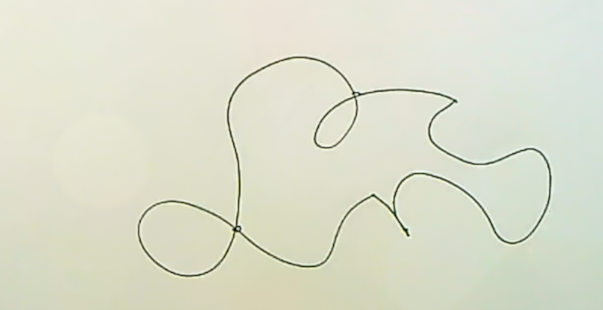
\includegraphics{figures/image_2020-11-27-21-49-40.png}
\caption{Image}
\end{figure}

These singular points are what stops \(A\) from being integrally closed,
which is literally true when \(k\) is a perfect field.

\end{remark}

Whereas \(\Sigma(K/k)\) is always infinite, \(\Sigma_1(K/k)\) by be
finite or even empty. When \(k = \QQ\), it may in fact be empty ``most
of the time'' When \(k = \QQ\), it may in fact be empty ``most of the
time''.

\begin{exercise}[?]

For all \(v\in \Sigma(K/k)\), the degree of the point \(\deg(v)\) will
be divisible by \([\kappa(K) : k]\). Thus if \(\kappa(L) \supsetneq k\),
then \(\Sigma_1(K/k) = \emptyset\).\footnote{Use the fact that the
  degree will be bigger than 1 when the constant field is bigger than
  \(k\).}

\end{exercise}

Note that before we were writing the residue field as an extension of
\(k\), and it's worth checking that the constant subfield embeds as a
subfield of the residue field as well.

\begin{remark}

There is a tie to CM points on modular curves: if you have a function
field over \(\QQ\) which is not regular due to some proper algebraic
subextension, the residue fields of all of the points on the curve will
contain the algebraic closure of the field of definition. Pete had some
\(\QQ(X_n)\) function field, whose constant subfield was
\(\QQ(\zeta_n)\) (adjoining the \(n\)th roots of unity), and none of
these modular curves over \(\QQ\) have closed points except when the
residue fields contain \(\QQ(\zeta_n)\).

\end{remark}

\begin{remark}

This is a way for there to not be points on the curve, so
\(\Sigma_1(K/k)\) is empty, but it's not the deepest reason -- this is a
cheap trick to produce ``pointless'' function fields. It can fail to
have degree 1 places in many different ways!

\end{remark}

\begin{exercise}[?]

Show that for for a one variable function field \(K/k\) TFAE:

\begin{enumerate}
\def\labelenumi{\arabic{enumi}.}
\item
  Every \(v\in \Sigma(K/k)\) has degree 1,
\item
  \(k\) is algebraically closed.
\end{enumerate}

\end{exercise}

\begin{remark}

One half is easy, since by definition the degree of the residue field is
the degree of some finite extension of the base field, but if \(k\) is
algebraically closed, the degree of any finite extension is one.

\end{remark}

\begin{exercise}[?]

For a field \(k\), set \(\PP^1(k) \da \PP(k^2)\), the projectivization
of \(k\cross k\), i.e.~the lines through the origin in \(\AA^2/k\). By
taking slopes of lines, \(\PP^1(k) = k \disjoint \ts{\infty}\).

\begin{figure}
\centering
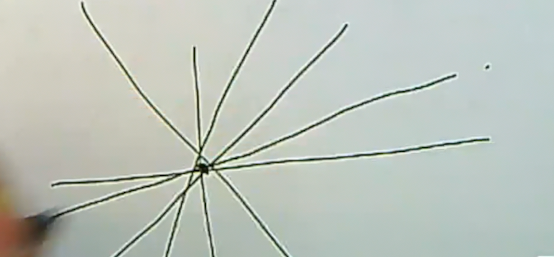
\includegraphics[width=3.64583in,height=\textheight]{figures/image_2020-11-27-23-57-12.png}
\caption{Image}
\end{figure}

Show that \(\Sigma_1(k(t)/k) = \PP^1(k)\), and deduce that
\begin{align*}  
\Sigma(k(t)/k) = \PP^1(k) \iff k = \bar k
.\end{align*}

\end{exercise}

Next up we'll talk about how the set of places is built from affine
Dedekind domains. After this, we'll be ready for chapter 2: divisors and
Riemann-Roch.

\hypertarget{lecture-5b-building-places-by-gluing-affine-dedekind-domains-todo}{%
\section{Lecture 5B: Building Places by Gluing Affine Dedekind Domains
(TODO)}\label{lecture-5b-building-places-by-gluing-affine-dedekind-domains-todo}}

\hypertarget{lecture-6}{%
\section{Lecture 6}\label{lecture-6}}

\hypertarget{lecture-8-riemann-roch-spaces}{%
\section{Lecture 8: Riemann-Roch
Spaces}\label{lecture-8-riemann-roch-spaces}}

Setting up for the single most important theorem in the course: the
Riemann-Roch theorem. We start by motivating this by considering the
following property of \(K\da k(t)\): for any degree 1\footnote{So the
  residue field of the corresponding DVR is \(k\) itself rather than
  some proper finite degree extension.} place \(p \in \Sigma(K/k)\),
there exists an \(f\in K\units\) such that \((f)_- = p\). In other
words, \(f\) is a rational function with a simple pole at the given
place, and no other poles. Why? We just know precisely what all of the
places are for this function field.

If \(p= \infty\), we can just take \(f(t) = t\), since any polynomial is
regular away from \(\infty\) and the valuation is \(-\deg(f) = -1\) The
other places \(p\) correspond to \(t-\alpha\) (the uniformizing element)
for \(\alpha\in k\), since they correspond to other points on
\(\AA^1_{/k}\), and so we can take \(f(t) = 1/(t-\alpha)\). This \(f\)
is regular at infinity since the degree of the numerator is larger than
the degree of the denominator, and the denominator doesn't vanish at any
other place.

\begin{remark}

With some thought, it can be found that this is a \emph{characteristic}
property of rational function fields: if \(f\in K\), a one variable
function field, and \(\deg(d)_- = 1\)\footnote{Recall that this is the
  divisor pole.} then the degree of the function is equal to the degree
of the divisor of the zeros and the divisor of the poles, and thus the
degree of the extension \([K: k(t)] = 1\) and thus \(K = k(t)\) is
rational. So having a rational with a simple pole at only one point
\emph{only} happens in you're in a rational function field.

On the other hand, we both wanted and used in our discussion of
holomorphy rings the fact that given a nonempty finite subset
\(S \subset \Sigma(K/k)\), we want to find a rational function
\(f\in K\units\) has poles at all of the points in \(S\), so
\(\supp (f)_- = S\). Better yet, we'd like a bound on the degree of any
such \(f\), i.e.~the orders of all of these poles. If \(S\) is a single
place, unless the function field is rational, we can't require the
function to have a pole of degree 1 at that point. But can it admit a
pole of degree at most 10, for example? This is what motivates the
Riemann-Roch spaces and the Riemann-Roch theorem. If you're trying to
give a quantitative bound on how high of an order of a pole you have to
allow in order to have a rational function, this comes from a key
invariant called the \emph{genus} of the function field. The theorem
that will tell us about the existence of rational functions with poles
of prescribed degrees in terms of the genus is precisely the
Riemann-Roch theorem, so that's where we are headed.

\end{remark}

\begin{definition}[Riemann-Roch Space of $D$ (Key Definition)]

For \(D\in \Div K\), the \textbf{Riemann-Roch space} of \(D\) is defined
as
\begin{align*}  
\mathcal{L}(D) \da \ts { f\in K\units \st (t) \geq - D} \union\ts{0}
.\end{align*}

\end{definition}

\begin{remark}

This will turn out to be a \(k\dash\)vector space, and is a sub
\(k\dash\)vector space of \(K\). One of the first things we'll prove is
that it's always finite dimensional. This is only interesting when \(D\)
is linearly equivalent to an effective divisor, so we should think of
\(D\) as having a nonnegative degree, and in fact itself being an
effective divisor. So this is the space of rational functions that have
prescribes poles of a prescribed order.

\end{remark}

\begin{question}

Does \(\mathcal{L}(D)\) contain any rational functions other than zero?

\end{question}

\begin{answer}

For any nonzero \(f\in \mathcal{L}(D)\nonzero\), the divisor \(D + (f)\)
is effective, since \((f) \geq -D\), and also linearly equivalent to
\(D\). If \(D\) is not linearly equivalent to an effective divisor, this
is just the zero vector space.

\end{answer}

\begin{exercise}[?]

Let \(K = k(t)\) and \(n\in \ZZ^{\geq 0}\). Show that
\begin{align*}
L(n\infty) = \ts{f\in k[t] \st \deg f \leq n}
\end{align*} and in particular is a \(k\dash\)vector space of dimension
\(n+1\).\footnote{Recall that \(\infty\) is the \(1/t\dash\)adic place.}

\end{exercise}

\begin{remark}

Note that \(\infty\) is a degree 1 place, and multiplying it by \(n\)
yields an effective divisor. The Riemann-Roch space here is comprised of
rational functions that regular away from \(\infty\), which are
polynomials, whose pole at \(\infty\) has order at worst \(n\). But the
order of a pole at infinity is its degree as a polynomial, since the
\(\infty\dash\)adic valuation is the negative degree, so this yields
polynomials of degree at most \(n\).

\end{remark}

\begin{lemma}[?]

For \(D\in \Div K\),
\begin{align*}  
\mathcal{L}(D) \neq \ts{0} \iff 0 \text{ is equivalent to an effective divisor}
.\end{align*}

\end{lemma}

\begin{proof}[?]

\(\implies\): If \(f\in \mathcal{L}(D)\nonzero\), then \(D + (f)\) is
effective and linearly equivalent to zero.

\(\impliedby\): If \(D' \geq 0\) and \(D' \sim D\), then
\(D' = D + (f) \geq 0\). So \((f) \geq -D\) and thus
\(f\in \mathcal{L}(D)\).

\end{proof}

\begin{example}[?]

\(\mathcal{L}(0) = \ts{f \st (f) \geq 0} \union\ts{0}\), which consists
of rational functions with no poles (so their divisor is the zero
divisor), and thus \(\mathcal{L}(0) = \kappa(K)\). I.e., these are the
constants: they are regular everywhere and have no zeros or poles. We
would like this space to have \(k\dash\)dimension 1, so we impose
\(\kappa(K) = k\).

\end{example}

\begin{exercise}[?]

\envlist

\begin{enumerate}
\def\labelenumi{\alph{enumi}.}
\tightlist
\item
  Show that for all \(D\), \(\mathcal{L}(D) \in \Vect_k\).
\item

  \begin{align*}  
  D\sim D' \implies \mathcal{L}(D) \cong_{\Vect_k} \mathcal{L}(D')
  .\end{align*}
\end{enumerate}

\end{exercise}

\begin{remark}

You can frame the above as taking rational functions with poles of
certain orders, and analyzing the orders of poles of their sums. If you
take \(D'\) and write it as \(D + (f)\) for \(f\) a rational function,
then \(f\) should produce this isomorphism. The moral:
\(\mathcal{L}(D)\) only depends on the linear equivalence class of
\(D\).

\end{remark}

\begin{exercise}[?]

Let \(D\in \Div^0 K\) be a degree zero divisor, then TFAE:

\begin{enumerate}
\def\labelenumi{\alph{enumi}.}
\tightlist
\item
  \(\dim \mathcal{L}(D) \geq 1\)
\item
  \(\dim \mathcal{L}(D) = 1\),
\item
  \(D\) is principal, i.e.~the divisor of a rational function or
  linearly equivalent to zero.
\end{enumerate}

\end{exercise}

\begin{slogan}

The only way a degree zero divisor can have a nontrivial Riemann-Roch
space is if it's linearly equivalent to zero.

\end{slogan}

\begin{lemma}[?]

Let \(A \leq B\)\footnote{These are formal linear combinations of
  places, so the coefficients in front of each place in \(A\) should be
  less than the corresponding coefficient for \(B\), or equivalently
  \(B-A\) is effective.} in \(\Div K\), then

\begin{enumerate}
\def\labelenumi{\alph{enumi}.}
\tightlist
\item
  \(\mathcal{L}(A) \leq_{\Vect_k} \mathcal{L}(B)\) is a subspace,
\item
  \(\dim \mathcal{L}(B) / \mathcal{L}(A) \leq \deg B - \deg A = \deg(B - A)\).
\end{enumerate}

\end{lemma}

\begin{remark}

Since \(B \geq A\), you can think of this as starting with \(A\) and
adding an effective divisor to get \(B\), namely \(A + (B-A) = B\). How
much does that decrease the dimension of the Riemann-Roch space? At
most, by the degree of \(B-A\) as a divisor.

\end{remark}

\begin{corollary}[?]

For \(D\in \Div K\),

\begin{enumerate}
\def\labelenumi{\alph{enumi}.}
\tightlist
\item
  If \(\deg D < 0\) then \(\mathcal{L}(D) = 0\).
\item
  If \(\deg (D) \geq 0\) then
  \(\dim_k \mathcal{L}(D) \leq \deg(D) + 1 < \infty\).
\end{enumerate}

\end{corollary}

\begin{remark}

This shows that Riemann-Roch spaces are always finite dimensional, and
also gives a simple upper bound on that dimension.

\end{remark}

\begin{proof}[of corollary]

For (a), a divisor of negative degree is not linearly equivalent to an
effective divisor, so we might as well assume it's effective.

For (b), the dimension of \(\mathcal{L}(D)\) doesn't change if \(D\) is
replaced by a linearly equivalent divisor, so wlog assume \(D\) is
effective. Now write \(D = \sum_{i=1}^r p_i\) as a sum of not
necessarily distinct places, and use the lemma: each time you add an
effective divisor, the dimension either stays the same or increases by
at most the degree of the added divisor. So start with the zero divisor,
use the fact that \(\dim_k \mathcal{L}(0) = 1\), and apply the lemma
\(r\) times. This yields a space of dimension at most
\(1 + \sum \deg p_i = \deg D\).

\end{proof}

\begin{proof}[of lemma, part (a)]

If \(A\leq B\) and \(f\in \mathcal{L}(A)\), then \((f) \geq - A\). Since
\(-A \geq -B\), we have \((f) \geq -A \geq -B\), so
\(f\in \mathcal{L}(B)\).

\end{proof}

For the next part, it's perhaps easiest to consider the case
\(k = \bar k\) so everything has degree 1. If you go from a divisor to
adding a single degree 1 place, this lemma says that if you increase
your Riemann-Roch space by either allowing a pole at a point you didn't
allow before or allowing a pole of order 1 greater, then the dimension
increases by at most 1.

\begin{proof}[of lemma, part (b)]

From the previous argument, we see that it's enough to do this one place
at a time. So we can easily reduce to the case \(B = A + P\) for \(P\)
some place of degree not necessarily equal to 1 (since we're not
assuming \(k=\bar k\)), using that fact that \(B \geq A\). So choose an
element \(t\in K\) such that
\begin{align*}  
v_p(t) = v_p(B) = v_p(A) + 1
,\end{align*} since \(B\) is built from \(A\) by adding a single copy of
\(P\). For \(f\in \mathcal{L}(B)\), we have by definition\footnote{Note
  that \(v_p\) is the \(p\dash\)adic valuation, i.e.~the coefficient of
  \(P\) in the divisor as a formal linear combination of points.}
\begin{align*}  
v_p(f) \geq -v_p(B) = -v_p(t)
,\end{align*} and so by bringing \(t\) to the other side we get
\(v_p(ft) \geq 0\) and thus \(ft\in R_p\) (the corresponding local
ring). This allows us to define a \(k\dash\)linear map
\begin{align*}  
\psi: \mathcal{L}(B) &\to k(P) = R_p/\mathfrak{m}_p \\
f & \mapsto ft \mod \mathfrak{m}_p
.\end{align*} In words, we multiply \(f\) by \(t\) to make it
\(p\dash\)adically regular, then look at its image in the residue field.
The kernel is precisely those elements \(x\) such that multiplying by
\(t\) lands in the maximal ideal \(\mathfrak{m}_p\), which means that
\(v(x)\) as 1 more than it could have been. So the kernel is all
elements such that multiplying by \(t\) and taking the valuation gives
at least one, thus
\begin{align*}  
\ker \psi = \ts{f\in \mathcal{L}(B) \st v_p(f) \geq -v_p(t) + 1 = -v_p(A)} = \mathcal{L}(A)
,\end{align*} which follows since \(B\) and \(A\) only differ at \(P\),
since \(B = A+P\), so the divisors \(A, B\) have the same coefficient at
every other place. We thus have the following diagram:

\begin{center}\begin{tikzcd}
    {0} & {\mathcal{L}(A)} & {\mathcal{L}(B)} & {\mathcal{L}(B)/\mathcal{L}(A)} & {0} \\
    \\
    {} & {} & {} & k(P) = {R_p / \mathfrak{m}_p} & {\cdots}
    \arrow[from=1-1, to=1-2, hook]
    \arrow[from=1-2, to=1-3, hook]
    \arrow[from=1-3, to=1-4, two heads]
    \arrow[from=1-4, to=1-5, two heads]
  \arrow[from=1-4, to=3-4, dotted, hook, "\exists \iota"]
    \arrow[from=1-2, to=3-4, "\psi"]
  \arrow[from=3-4, to=3-5]
\end{tikzcd}\end{center}

\href{https://q.uiver.app/?q=WzAsMTAsWzAsMCwiMCJdLFsxLDAsIlxcbWF0aGNhbHtMfShBKSJdLFsyLDAsIlxcbWF0aGNhbHtMfShCKSJdLFszLDAsIlxcbWF0aGNhbHtMfShCKS9cXG1hdGhjYWx7TH0oQSkiXSxbNCwwLCIwIl0sWzAsMiwiMCJdLFsxLDIsIlxcbWF0aGNhbHtMfShBKSJdLFsyLDIsIlxcbWF0aGNhbHtMfShCKSJdLFszLDIsIlJfcCAvIFxcbWF0aGZyYWt7bX1fcCJdLFs0LDIsIlxcY2RvdHMiXSxbMCwxLCIiLDAseyJzdHlsZSI6eyJ0YWlsIjp7Im5hbWUiOiJob29rIiwic2lkZSI6InRvcCJ9fX1dLFsxLDIsIiIsMCx7InN0eWxlIjp7InRhaWwiOnsibmFtZSI6Imhvb2siLCJzaWRlIjoidG9wIn19fV0sWzIsMywiIiwwLHsic3R5bGUiOnsiaGVhZCI6eyJuYW1lIjoiZXBpIn19fV0sWzMsNCwiIiwwLHsic3R5bGUiOnsiaGVhZCI6eyJuYW1lIjoiZXBpIn19fV0sWzEsNiwiIiwwLHsic3R5bGUiOnsiaGVhZCI6eyJuYW1lIjoibm9uZSJ9fX1dLFsyLDcsIiIsMCx7InN0eWxlIjp7ImhlYWQiOnsibmFtZSI6Im5vbmUifX19XSxbMyw4LCIiLDAseyJzdHlsZSI6eyJ0YWlsIjp7Im5hbWUiOiJob29rIiwic2lkZSI6InRvcCJ9LCJib2R5Ijp7Im5hbWUiOiJkb3R0ZWQifX19XSxbMCw1LCIiLDIseyJzdHlsZSI6eyJoZWFkIjp7Im5hbWUiOiJub25lIn19fV0sWzYsNywiIiwxLHsic3R5bGUiOnsidGFpbCI6eyJuYW1lIjoiaG9vayIsInNpZGUiOiJ0b3AifX19XSxbNyw4XSxbNSw2LCIiLDIseyJzdHlsZSI6eyJ0YWlsIjp7Im5hbWUiOiJob29rIiwic2lkZSI6InRvcCJ9fX1dLFs4LDldXQ==}{Link
to diagram}

where we can conclude that the indicated injection exists, and thus
\begin{align*}  
\dim \mathcal{L}(B) / \mathcal{L}(A) \leq [k(p) : k] = \deg P
.\end{align*}

\end{proof}

\begin{fact}

For \(p\in \Sigma(K/k)\) with residue field \(k_p\) and
\([k_p: k] = d\), defining \(K_p\) as the completion of \(K\) with
respect to \(\abs{\wait}_p\), there is an isomorphism
\(K_p \cong k_p((t))\), a formal Laurent series field. One issue is that
if \(d =1\) then \(k \subset k_p\), but not for general \(d\geq 2\).
However, taking the completion results in \(k \subset K_p\) again. This
shouldn't be too surprising from the perspective of local fields in
NTII. There is a structure theory of complete discretely valued fields.
This is an \emph{equicharacteristic} such field, i.e.~the characteristic
of the field agrees with that of the residue field, and all
equicharacteristic discretely valued fields will be isomorphic to a ring
of formal Laurent series. This isn't a fact of the geometry of curves.

\end{fact}

\begin{definition}[?]

For \(D\in \Div K\), define
\begin{align*}  
\ell(D) \da \dim_k \mathcal{L}(D)
.\end{align*}

\end{definition}

\begin{exercise}[?]

If \(D\in \Div k(t)\), show that
\begin{align*}  
\ell(D) = 
\begin{cases}
\deg(D) + 1 & \deg D \geq 0 \\
0 & \text{else}.
\end{cases}
\end{align*}

\end{exercise}

\begin{remark}

Recall that in a rational function field, every degree zero divisor is
principal, and if you adjust by a principal divisor, you don't change
\(\ell(D)\). This means that in any rational function field, any two
divisors of the same degree are going to be linearly equivalent, and
thus \(\ell(D)\) will only depend on \(\deg D\). So rational function
fields are much simpler than the fully general case.

\end{remark}

\begin{problem}[The Riemann-Roch Problem]

Give good upper and lower bounds on \(\ell(D)\) and especially
\(\ell(nD)\) as a function of \(n\).

\end{problem}

\begin{remark}

The stronger version of knowing \(\ell(D)\) in all cases is unsolvable.
If we knew the dimension of every Riemann-Roch space, then we would know
too much! E.g. about Weierstrass points on elliptic curves. (?) Looking
at positive multiples \(nD\) of a single divisor is common. If \(D\) is
a single point, then the support of the divisor is the collection of
places that appear with nonzero coefficients, \(nD\) has the same
support. This is analogous to not allowing poles at new points, but
rather allowing poles at the same points of higher order. So it's
reasonable to ask about asymptotic behavior of \(\ell(nD)\) in \(n\).
Secretly this is a kind of Hilbert function computation: if you have a
graded algebra and you look at dimensions of its graded pieces, then
there is a theorem that the Hilbert function is a polynomial for
\(n\gg 1\). Here, \(\ell(nD)\) will be a linear polynomial for
\(n\gg 1\) by the Riemann-Roch theorem, so there are some stabilization
phenomena, but given a random divisor of low degree it is difficult to
determine \(\ell(D)\).

\end{remark}

\begin{remark}

The last corollary gave us a lower bound:
\begin{align*}  
\deg(D) \geq 0 \implies \deg(D) - \ell(D) \geq -1
.\end{align*} This can also be thought of as an lower bound on
\(\ell(D)\) in terms of \(\deg(D)\), and next up we'll try to find an
upper bound:

\end{remark}

\begin{proposition}[]

There exists a \(\delta = \delta(K/k) \in \ZZ\) such that for all
\(A\in \Div K\), we have
\begin{align*}  
\deg A - \ell(A) \leq \delta
.\end{align*}

\end{proposition}

\hypertarget{lecture-10-todo}{%
\section{Lecture 10 (Todo)}\label{lecture-10-todo}}

\hypertarget{lecture-11a-weils-proof-of-riemann-roch}{%
\section{Lecture 11A: Weil's Proof of
Riemann-Roch}\label{lecture-11a-weils-proof-of-riemann-roch}}

Let \(K_{/k}\) be a one variable function field, finitely generated of
transcendence degree one, with \(\kappa(K) = k\), so \(k\) is
algebraically closed in \(K\). Define the \emph{small Adele ring}
associated to \(K\), as the restricted direction product with respect to
\(\ts{R_v \st v\in \Sigma(K/k)}\):

\begin{align*}
A_k \da \prod^{\text{res}}_{v\in \Sigma(K/k)} K
= \ts{(x_v) \in K^{\Sigma(K/k)} \st x_v \in R_v \text{ for a.e. } v }
,\end{align*} where each factor is a copy of \(K\). Note that a
\emph{restricted} direct product is when you have a family of sets, and
for each set you also attach a subset. Then if you have a tuple in the
entire direct product, it's in the restricted direct product iff for all
but finitely many coordinates lie in a given subset. Here the subset is
the valuation ring \(R_v\). So these are tuples of elements of \(K\),
indexed by places, where each element has a \(p\dash\)adic valuation and
the only restriction is that (except for finitely many cases) we want
this valuation to be nonnegative.

\begin{remark}

To get the \emph{big} Adele ring, you'd replace \(K\) with its
completion with respect to the \(p\dash\)adic valuation. If \(k\) is
finite, then this is equal to the positive characteristic Adele ring
from NTII. If you complete, then you get a complete discretely valued
field whose residue field equals the residue field at the place \(v\).
So for finite extensions of \(k\), the residue will be finite iff \(k\)
is finite, and from the structure theory of discretely valued fields,
this field has a natural topology: the adic topology, coming from the
inverse limit. This will be locally compact iff the residue field is
finite. Here, since the ground field is infinite, even passing to the
completion wouldn't yield anything locally compact. So there's no
advantage to passing to the completion, although there's no harm either.

\end{remark}

Note that \(A_k\) is a ring, and in fact a \(K\dash\)algebra, but we
will only need its structure as a \(K\dash\)vector space. This structure
comes from embedding \(K\injects A_k\) diagonally, so
\(x \mapsto [x, x, \cdots]\), and pull back \(v\in \Sigma(K/k)\),
remembering that every element of \(K\) (a rational function) is regular
except for finitely many \(v\).

If we have a valuation on \(K\), we can consider a place \(p\) and
projecting onto the \(k\)th factor:
\begin{align*}  
A_j \surjectsvia{\pi_p} K \mapsvia{v_p} \ZZ \union \ts{\infty}
.\end{align*}

So we now attach an adelic version of the Riemann-Roch space: for
\(D\in \Div K\), we set
\begin{align*}  
\mathcal{A}_k(D) \da \ts{ \alpha \in \mathcal{A}_K \st v_p(\alpha) \geq -v_p(D) \, \forall p \in \Sigma(K/k)}
.\end{align*} The only difference here is that the usual space is over
\(K\), and here we're over \(\mathcal{A}_K\), which is a much larger
space. This makes things easier, however, in the same sense that
studying a large collection of local fields is easier than studying the
corresponding global field. Note that the \(p\dash\)adic valuation
\(v_p\) is just the coefficient of \(p\) in the divisor, and
\(\mathcal{A}_K \intersect K\) yields the usual Riemann-Roch space.

\begin{exercise}[?]

\envlist

\begin{enumerate}
\def\labelenumi{\alph{enumi}.}
\item
  Show that \(\mathcal{A}_K(D)\) is an \(k\dash\)subspace of
  \(\mathcal{A}_K\).\footnote{Consider scaling by nonzero constants,
    where the valuation of constants are zero.}
\item
  Show that (just as for the Riemann-Roch space)
  \(D_1 \leq D_2 \implies \mathcal{A}_K(D_1) \subseteq \mathcal{A}_K(D_2)\).
\end{enumerate}

\end{exercise}

\begin{lemma}[?]

\begin{align*}  
D_1 \leq D_2 \implies \dim_k \mathcal{A}_K(D_2) / \mathcal{A}_K(D_1) = \deg D_2 - \deg D_1
.\end{align*}

\end{lemma}

Note that this is the adelic analogue of our first lemma on Riemann-Roch
spaces, now with an equality instead of being bounded above.

\begin{proof}[?]

As we did before, by induction we can assume \(D_2 = D_1 + p\) for some
\(p\in \Sigma(K/k)\), i.e.~we can go from the smaller divisor to the
bigger one by repeatedly adding closed points. Then choose an element
\(t\in k\units\) such that \(v_p(t) = v_p(D_2)\), and define a similar
map
\begin{align*}  
\phi \mathcal{A}_K(D_2) &\to k_p \\
\alpha &\mapsto (t\alpha p) \mod \mfm_p
.\end{align*} Why? Once you multiply by \(t\), note that we're looking
in the \(p\)th component. The condition before was that the valuation at
the \(p\)th component was at least \(-v_p(D_2)\), but now we're adding
\(v_p(D_2)\). This yields a nonnegative valuation, making the image lie
inside the corresponding local ring, so it makes sense to consider it
modulo the maximal ideal to get an element of the residue field. As
before, it should be clear that this is \(k\dash\)linear,
\(\ker \phi = \mathcal{A}_K(D_1)\), and is surjective. The kernel are
exactly those elements such that multiplying by \(t\) makes the
\(p\dash\)adic valuation at least 1, since that's what the maximal ideal
is. This is indeed \(\mathcal{A}_K(D_1)\), since \(D_1\) and \(D_2\) are
the same except for the added condition \(D_2 = D_1 + p\) at \(p\).\\

So the main difference is that the map is now \emph{surjective}, which
was not true for the original Riemann-Roch space. Why? This is a purely
local situation. Take an element which is zero away from the \(p\)
component, which is easy to do since zero is in \(R_v\) for any \(v\).
So can you find an element of \(k\) such that multiplying by \(t\) and
reducing modulo the maximal ideal yields every element of the residue
field?

\end{proof}

\begin{theorem}[2.13]

For all \(D\),
\begin{align*}  
\dim_k \mathcal{A}_K / \qty{\mathcal{A}_K(D) + K } = \iota(D) \da \ell(D) - \deg(D) + g - 1
,\end{align*} where \(\iota(D)\) is the index of speciality of the
divisor, which measures the discrepancy between the degree and the
dimension.

\end{theorem}

\begin{remark}

This says that adding \(K\) into the adelic Riemann-Roch space results
in a big \(k\dash\)vector space, having high dimension in the infinite
dimensional \(k\dash\)vector space \(\mathcal{A}_K\).

\end{remark}

\begin{proof}[Step 1]

For divisors \(A_1 \leq A_2\), we have a short exact sequence of
\(k\dash\)vector spaces
\begin{align*}  
0 \to \mathcal{L}(A_2) / \mathcal{L}(A_1) \mapsvia{\sigma_1} \mathcal{A}_K(A_2) / \mathcal{A}_K(A_1) \mapsvia{\sigma_2} \qty{\mathcal{A}_K(A_2) + K} / \qty{\mathcal{A}_K(A_1) + K } \to 0
.\end{align*} The first thing we did was compute the dimension of the
middle quotient space, which was \(\deg D_2 - \deg D_1\). Note that
\(\sigma_2\) is a quotient map, but \(\sigma_1\) just comes from
embedding \(K\injects \mathcal{A}_K\). To show exactness, the only
nontrivial part is that \(\ker(\sigma_2) \subset \im(\sigma_1)\). So
take an element \(\alpha\in \mathcal{A}_K(A_1) \mod \mathcal{A}_K(A_1)\)
such that \(\sigma_2(\alpha) = 0\), so there exists an \(x\in K\) such
that \(\alpha-x \in \mathcal{A}_K(A_1)\) by definition of being zero in
the last quotient. Since
\(\mathcal{A}_K(A_1) \subseteq \mathcal{A}_K(A_2)\), we have that
\(x\in \mathcal{A}_K(A_2) \intersect K \da \mathcal{L}(A_2)\). This
follows because \(\alpha, \alpha-x\) are both in \(\mathcal{A}_K(A_2)\).
Thus we have
\begin{align*}  
\alpha + \mathcal{A}_K(A_1) = x + \mathcal{A}_K(A_1) = \sigma\qty{x + \alpha(A_1)}
.\end{align*}

\end{proof}

\begin{proof}[Step 2]

We can now compute the dimension of this quotient. Using step 1 and
Lemma 2.12, we get
\begin{align*}  
\dim_k\qty{ \mathcal{A}_K(A_2) + K } / \qty{ \mathcal{A}_K(A_1) + K }
&= \dim_k \mathcal{A}_K(A_2) / \mathcal{A}_K(A_1) - \dim_k \mathcal{L}(A_2) / \mathcal{L}(A_1) \\
&= \qty{\deg A_1 - \ell(A_2) } - \qty{\deg A_1 - \ell(A_1) } \\
&= \iota(A_1) - \iota(A_2)
,\end{align*} where the last step follows from adding and subtracting
\(g-1\).

\end{proof}

\begin{proof}[Step 3]

By step 2, it is enough to show that for all \(A_1 \in \Div K\), there
exists a bigger divisor \(A_2 \geq A_1\) such that \(\iota(A_2) = 0\)
(by just adding closed points) and
\(\mathcal{A}_K(A_2) + K = \mathcal{A}_K\). By Riemann's inequality, we
have \(\iota(A_2) =0\) if \(\deg A_2 \gg 0\), so choose such an
\(A_2 \geq A_1\). Thus we're reduced to showing that if \(\iota(B) = 0\)
for all \(B\in \Div K\), then \(\mathcal{A}_K = \mathcal{A}_K(B) + K\).
We'll do this by choosing another large effective divisor.\footnote{This
  ``cone structure'' on divisors is very useful!}

Let \(B_1 \geq B\), then we have
\begin{align*}  
\ell(B_1) 
&\leq \deg(B_1) + \ell(B) - \deg(B) \\
&= \deg(B_1) - g + 1
.\end{align*} Also, Riemann's inequality gives
\(\ell(B_1) \geq \deg(B_1) - g + 1\), so we have equality. Thus any
divisor greater than or equal to a non-special divisor is again
non-special.\\

We want to take an arbitrary element of the Adele ring and show that it
differs from an element of the adelic Riemann-Roch space associated to
\(B\) by an element of \(K\), so we'll cleverly choose a divisor in
order to do this. So take an arbitrary element
\(\alpha\in \mathcal{A}_K\) of the Adele ring, then we may choose
\(B_1 \geq B\) such that \(\alpha\in \mathcal{A}_K(B_1)\). I.e.,
choosing \(B_1\) large enough is allowing the poles to be however bad
you want them to be, and \(\alpha\) is a fixed element, all but finitely
many elements have valuation \(\geq 0\).

We understand the relative situation well, based on what we proved. By
step 2, since \(B, B_1\) are non-special, the dimension of the quotient
is zero:
\begin{align*}  
\dim_k(\mathcal{A}_K(B_1) + K) / (\mathcal{A}_K(B) + K) 
&= \deg \qty{B_1 - \ell(B_1)} - \qty{\deg B - \ell(B) } \\
&= (g-1) - (g-1) \\
&= 0
.\end{align*} But then these spaces are equal to each other, so
\(\mathcal{A}_K(B_1) + K = \mathcal{A}_K + K\). But we chose \(B_1\)
arbitrarily large so it contained \(\alpha\), and we found that the
resulting space is no bigger than the original. Note that \(B_1\) was
chosen so that \(\alpha\in \mathcal{A}_K(B_1)\) before adding \(K\),
which remains true when adding \(K\). But this says \(\alpha\) is in the
LHS, which equals the RHS. Then \(\alpha \in \mathcal{A}_K(B)\), where
\(\alpha\) was arbitrary, so \(\alpha\in \mathcal{A}_K(B) + K\).

\end{proof}

\begin{corollary}[2.14]

This can be applied to the zero divisor:
\begin{align*}  
\dim_k \mathcal{A}_K( \mathcal{A}_K(0) + K ) \iota(0) = g
.\end{align*}

\end{corollary}

\begin{exercise}[?]

Corollary 2.14 shows that if \(K = k(t)\) is the rational function
field, then we have \(\mathcal{A}_K(0) + K = \mathcal{A}_K\).\footnote{So
  every Adele differs from a rational function by an effective Adele.}
Show this directly.

\end{exercise}

\begin{remark}

Note that analogy to consider \(\mathcal{A}(\QQ)\), where you get
\(\mathcal{A}_\QQ = \hat \ZZ + \QQ\), where \(\hat \ZZ\) denotes the
profinite completion. Recall that
\(\AA_\QQ = \prod_p' \QQ_p \cross \RR\), and inside of this we have
\(\AA(0) \da \prod_p \ZZ_p \cross \RR\). Not too crazy of a fact: given
an Adele, it has finitely many places where its \(p\dash\)adic valuation
is negative, so it shouldn't be hard to find a rational number as a
correction term which doesn't change the valuation. The fact that this
works for \(\QQ\) is related to \(\ZZ\) being a PID.

\end{remark}

\hypertarget{lecture-11b-weils-proof-of-riemann-roch-todo}{%
\section{Lecture 11B: Weil's Proof of Riemann-Roch
(TODO)}\label{lecture-11b-weils-proof-of-riemann-roch-todo}}

\hypertarget{lecture-11c-weils-proof-of-riemann-roch-todo}{%
\section{Lecture 11C: Weil's Proof of Riemann-Roch
(TODO)}\label{lecture-11c-weils-proof-of-riemann-roch-todo}}

\hypertarget{lecture-12-chapter-3-curves-over-a-finite-field}{%
\section{Lecture 12 (Chapter 3: Curves Over a Finite
Field)}\label{lecture-12-chapter-3-curves-over-a-finite-field}}

\hypertarget{section}{%
\subsection{}\label{section}}

We consider \(k= \FF_q\) a finite field, which by definition is a one
variable global function field. Idea: we've defined some affine dedekind
domains (the holomorphy rings) had a finite nonempty set of places of
the function field. These are analogous to the ring of integers of a
number field, or more generally \(S\dash\)integer rings. Recall some
basic results from NT1: the finiteness of the class group, and the
finite generation of the unit group. Here we have a class groups of
affine Dedekind domain, and by Rosen's theorem, there are infinitely
many as you vary over nonempty subsets of places of the function field,
and they're all closely connected to a geometric class group: the degree
zero divisor class group. Thus by this analogy, when the field is
finite, we'd expect that \(\Cl^0(K)\) is finite as well, which is the
main result we'll prove today.

\hypertarget{base-extension-1}{%
\subsection{Base Extension}\label{base-extension-1}}

Let \(K_{/\FF_q}\) be a one variable function field with constant field
\(\FF_q\), so that the only elements of \(K\) that are algebraic over
\(\FF_q\) are already in \(\FF_q\). Since \(\FF_q\) is a perfect field
(\(x\mapsto x^p\) is a surjection), every such function field is
regular.

Let \(\bar{\FF}_q\) be an algebraic closure, then for all \(r\in \ZZ^+\)
there exists a unique degree \(r\) extension, which we'll denote
\(\FF_{q^r}\). The extension \(\FF_{q^r}/\FF_q\) is a cyclic galois
extension (i.e.~it's galois group is cyclic) with a canonical generator:
the Frobenius map.

The galois theory of the constant field comes in when trying to study
constant extensions of the function field. There is a general theory of
constant extensions, but in our case, every such extension will be
cyclic or procyclic, so we don't need the entire theory.

For any positive integer \(r\), define the extension
\(K_r \da K \FF_{q^r}\) given by extending scalars, which is a regular
function field over \(\fqr\). There are two ways to obtain this: either
take an algebraic closure of \(K\) and take the compositum, or take
\(K\tensor_{\fq}\fqr\), which we proved was again a field. This \(K_r\)
is what we get by extending constants, and the way regular function
fields work is that if you make an arbitrary extension of the ground
field, then you retain a regular function field over this new extension.
On the other hand, note that \(K_R/K\) is a degree \(r\) arithmetic
extension of function field, whose galois group is also generated by
Frobenius. If we take any regular function field over \(k\) and then
take a finite galois extension \(l/k\), then extending scalars in this
way would give an extension of the upstairs fields which is galois and
has the same galois group as the constant extension. This is
\emph{arithmetic} because the only thing that changes going from \(K\)
to \(K_r\) is the field of constants.

In the analogy of function fields as the meromorphic functions on a
Riemann surface, this type of extension has no analog: since \(\CC\) is
algebraically closed, there are no constant extensions. So arithmetic
extensions are just extending scalars, and \emph{geometric} extensions
don't change the constant field at all and instead have the property
that if you extended scalars to the algebraic closure, you'd have an
extension of the same degree. Note that the étale fundamental group also
has a similar decomposition into an arithmetic part and a geometric part
(see Daniel Litt's course).

\hypertarget{splitting-of-places}{%
\subsubsection{Splitting of Places}\label{splitting-of-places}}

\begin{question}

Given a place in \(K\), how does it split (or not) in \(K_r\)?

\end{question}

\begin{remark}

We can ask this question in whenever we have an extension of function
fields. This reduces to the usual ATI type of question: for
\(v\in \Sigma(K/\fq)\), choose an affine Dedekind domain \(R\) such that
\(v\in \Sigma(K/R)\), i.e.~the place is regular. Let \(S\) be the
integral closure of \(K\) in \(K_r\); this place corresponds to a
maximal ideal \(\mathfrak{p}\), we then want to factor its pushforward
\(\mathfrak{p}_v S\). So this question is a special case of how a prime
ideal factors in an extension of Dedekind domains.

\end{remark}

We'll temporarily black-box the following lemma:

\begin{lemma}[?]

Suppose \(v\) is the downstairs place, \(r\) is the degree of the
extension, and \(d\da \deg(v)\). Then

\begin{itemize}
\item
  \(K_r/K\) is galois and we have \(efg = r\).\footnote{\(e\) is the
    prime ramification index, \(f\) is the prime residual degree, and
    \(g\) is the number of distinct primes. This result essentially
    comes from ANTI, replacing \(\sum e_i f_i = r\).}
\item
  This extension will be unramified: we in fact have \(e=1\), so
  \(g = \gcd(d, r)\) and \(f = r/\gcd(d, r)\), and
\item
  Each place \(w\in \Sigma(K_r/\fqr)\) lying over \(v\) has degree
  \(d/\gcd(d, r)\).
\end{itemize}

\end{lemma}

\begin{remark}

Note that having an extension of Dedekind domains coming from a galois
extension of fields simplifies things: this makes the inertial degree
and ramification indices coincide.

\end{remark}

\begin{example}[?]

\envlist

\begin{itemize}
\item
  The extension is inert \(\iff\) \(\gcd(d, r) = 1\)

  \begin{itemize}
  \tightlist
  \item
    I.e. \(d, r\) are coprime and \(g=e=1, f=r\).
  \end{itemize}
\item
  The extension splits completely \(\iff\) \(r \divides d\).

  \begin{itemize}
  \tightlist
  \item
    If \(r=d\), i.e.~we take a degree \(d\) place and extend scalars to
    \(K_d\), it splits completely into \(d\) degree 1 places.
  \end{itemize}
\item
  All \(w\divides v\) have degree 1 \(\iff\) \(d\divides r\).
\end{itemize}

\end{example}

\begin{remark}

Suppose we have \(w\) over \(v\) with \(w\in \Sigma(\fqr)\) and
\(v\in \Sigma(K/\fq)\). If \(v\) has degree \(d\), this means that the
residue field satisfies \(k(v) \cong \FF_{q^{d}}\), since we have unique
extensions in each degree. If \(f\) is the \(f\) from ANTI, it is also
the degree of the residual extension, so we know \([k(w): k(v)] = f\)
and thus \(k(w) \cong \FF_q^{f d}\).

On the other hand, \(k(w)\) is an extension of \(\fqr\) of degree
\(\deg(w)\), so
\(k(w) \cong \FF_{ \qty{q^r}^{\deg(w)} } = \FF_{q^{r\deg(w)}}\). Thus
\(r=fg\) and
\begin{align*}  
q^{f\deg(v)} = q^{r\deg(w)} \implies \deg(w) = \qty{f\over r}\deg(v) = { \deg(v) \over g}
.\end{align*}

The residue field, if it changes at all, can only increase in size,
since any extension of Dedekind domains induces an extension of residue
fields. So the size of the residue field of \(w\) is at least as big as
the size of the residue field of \(v\). But the degree of \(w\) is
measured relative to the extended field \(\fqr\), since it's the degree
of the residue field as an extension of \(\fqr\). So consider
\(\deg(w) = \deg(v)/g\), we see that even as the residue field is
increasing by a factor of \(f\), the degree of the point is decreasing
by a factor of \(g\).

\textbf{Upshot}: The residue field grows, but its degree can only
shrink. Thus making an extension forces the degrees of the upstairs
places to \emph{decrease}.

\end{remark}

We're trying to find out in how many ways a discrete valuation extends
to a finite degree field extension. From ANTII, we have a result that
describes this: if \(v\) is a rank 1 valuation on \(k\) and \(L/K\) is a
finite degree extension, then the extensions of \(v\) to \(L\)
correspond with \(\mspec(\hat{K}_v \tensor_K L)\), where the hat denotes
completing \(K\) with respect to the valuation. The \(e,f,g\) can all be
computed as well.\footnote{See Pete's NTII notes, Theorem 1.64.}

This is some finite degree \(\hat{K}_v\) algebra, and if \(L/K\) is
separable then this decomposes as a finite product of finite degree
field extensions of \(K\) and \(\hat{K}_v\), the number of which will be
\(g\). The \(e\) and \(f\) can be read off because each extension will
have a ramified and unramified part.

\begin{exercise}[?]

\envlist

\begin{enumerate}
\def\labelenumi{\alph{enumi}.}
\item
  Show that \(\FF_{q^d} \tensor_{\FF_q} \FF_{q^r} \cong \FF_{q^l}^{d'}\)
  where \(l = \lcm(d, r)\) and \(d' = \gcd(d, r)\).
\item
  Generalize this to the case when \(k_p / k\) and \(\ell / k\) are both
  cyclic galois extensions.
\end{enumerate}

\end{exercise}

\hypertarget{degree-1-places-and-rational-points-on-a-curve}{%
\subsection{Degree 1 Places and Rational Points on a
Curve}\label{degree-1-places-and-rational-points-on-a-curve}}

Taking the lemma as a black box, for \(r\in \ZZ^+\) let
\(N_r \da \abs{\Sigma_1(K_r/ \fqr) }\), i.e.~the number of degree 1
places of the function field after making a degree \(r\) extension.
Equivalently, \(N_r = \abs{C(\fqr)}\) where \(C\) is a unique complete
nonsingular curve over \(\fq\) corresponding to \(K\), and this denotes
the number of \(\fqr\) rational points. We'll eventually see these are
finite.

\begin{remark}

Important way of thinking about these: degree one places of a function
field over \(k\) correspond to \(k\dash\)rational points of a curve.

\end{remark}

\begin{corollary}[Equivalence of data: places and rational points]

\begin{align*}  
N_r = \sum_{d\divides r} d\cdot \abs{\Sigma_d(K/ \fq)}
,\end{align*} so knowing the number of closed points of each degree is
equivalent to knowing the \(\fqr\dash\)points for all \(r\).

\end{corollary}

\begin{proof}[?]

Let \(w\in \Sigma_1(K_r/\fqr)\) be a degree 1 point and set
\(v \da w\intersect K\) so \(w\) lies over \(v\). What is the degree of
\(v\)? Setting \(d \da \deg(v)\), the lemma gives
\begin{align*}  
1 = \deg(w) = {d\over \gcd(d, r)}
,\end{align*} which implies that \(\gcd(d, r) = d\) and thus
\(d\divides r\). So for each \(d\) dividing \(r\), every degree of
\(v\in \Sigma(K/\fq)\) contributes \(\gcd(d, r) = d\) degree 1 points on
\(K_r\), i.e.~every downstairs degree \(d\) place splits into \(d\)
degree one places. So for every such \(d\), every degree \(d\) closed
point contributes \(d\) degree 1 closed points lying above it, and
conversely if \(d\) does not divide \(r\) then the upstairs point would
not have degree 1, so this accounts for all of the degree 1 points.

\end{proof}

\begin{remark}

We saw that the degree 1 places and the rational points are the same
information, and there is a third equivalently quantity: \(A_n\),
defined to be the number of effective divisors of degree \(n\).

\end{remark}

\hypertarget{finiteness-of-places-and-rational-points}{%
\subsection{Finiteness of Places and Rational
Points}\label{finiteness-of-places-and-rational-points}}

\begin{lemma}[?]

\envlist

\begin{enumerate}
\def\labelenumi{\alph{enumi}.}
\item
  For all \(d\), the number of degree \(d\) closed points
  \(\Sigma_d(K/\fq)\) is finite (and therefore \(N_r\) is finite), and
\item
  For all \(n\), \(A_n\) is finite.
\end{enumerate}

\end{lemma}

\begin{proof}[of a]

Let \(L/K\) be a degree \(n\) extension of regular function fields over
\(\fq\). We then have a restriction map
\begin{align*}  
r: \Sigma(L/\fq) \surjects \Sigma(K/\fq)
\end{align*} which we showed is surjective with finite fibers. We can
say a little bit more: for all places \(w \in \Sigma(L/\fq)\), we have
an inequality
\begin{align*}  
\qty{1\over n}\deg(w) \leq \deg(r(w)) \leq \deg(w)
,\end{align*} noting that we're now measuring all degrees over a common
ground field \(\fq\). So things are now what you'd expect: the degree of
the upstairs point is a multiple of the degree of the downstairs point.
The upper bound comes from the fact that the residue of the upstairs
point is a finite extension of the residue field of the downstairs
points. The opposite inequality comes from ANTI: the degree of the
residual extension is at most the degree of the entire extension.

So \(r\) doesn't preserve degrees exactly, but preserves them up to a
bounded factor, and thus \(\Sigma_{\leq d}(L/\fq)\) is finite for all
\(d\) \(\iff\) \(\Sigma_{\leq d}(K/\fq)\) is finite for all \(d\).
Because of this, we can reduce the situation by exchanging the function
field \(L/\fq\) with any other function field for which \(L\) is a
finite extension, and in particular we can take the rational function
field \(K = \FF_q(t)\). What are the degree \(d\) places of a rational
function field? There is exactly one place at infinity, and the
remaining ones correspond to monic irreducible polynomials. Since
\(\fq\) is finite, there are only finitely many such polynomials of any
fixed degree.\footnote{There is an exact formula for this quantity.}

\end{proof}

\begin{proof}[of b]

Left as an exercise.

Some remarks: how do you build an effective divisor of degree \(n\)?
Take closed points (places) and start adding them up with positive
coefficients, then the degree of the divisor is the sum of the degrees
of the places. But if you only have finitely many places, each of which
can only be used a bounded number of times (certainly no more than \(n\)
times!), thus one can only build finitely many effective divisors of
each degree.

\end{proof}

\hypertarget{finiteness-of-class-group}{%
\subsection{Finiteness of Class Group}\label{finiteness-of-class-group}}

\begin{proposition}[Finiteness of class group]

The degree 0 divisor class group \(\Cl^0(K)\) is finite.

\end{proposition}

This is a geometric analog of the finiteness of the class group of the
ring of integers of a number field. By Rosen's theorem, as an immediate
corollary, the class group of any affine dedekind domain over a finite
ground field is finite. This follows from looking at the exact sequence:
a finite index subgroup of the class group of any dedekind domain is a
quotient of \(\Cl^0(K)\), and a finite index subgroup of a finite group
is finite.

\begin{proof}[?]

Set \(\delta \da I(K)\) to be the index, i.e.~the least possible degree
of a divisor.\footnote{By a theorem of Schmidt, we'll later prove that
  \(\delta = 1\).}

In any case, for all \(n\in \ZZ\), we have
\begin{align*}  
\Cl^n K = 
\begin{cases}
0 & \delta\notdivides n \\
\abs{\Cl^0 K} & \delta\divides n
\end{cases}
.\end{align*} If you have any degree \(n\) divisors, then \(\Cl^n K\)
will be a coset of \(\Cl^0 K\). Here we just look at the degree map,
which is a group morphism onto its image, of which all nonempty fibers
have the same size. Thus we may work with \(\Cl^n K\) for \(n\gg 0\).\\

In particular, choose \(n\geq g\) the genus such that
\(\delta \divides n\), and let \(D \in \Div^n K\). A Riemann-Roch
computation shows that \(\ell(D)\), the dimension of the linear system,
is at least \(n-g+1\), and so we have \(\ell(D) \geq 1\) and \(D\) is
linearly equivalent to an effective divisor. This shows that the map
taking effective degree \(n\) divisors to \(\Cl^n K\) taking a divisor
to its divisor class (restricted to effective divisors) is surjective.
But we just saw that the set of effective degree \(n\) divisors is
finite -- it was built out of finitely many closed points of bounded
degrees -- forcing \(\Cl^n K\) to be finite. The result follows because
\(\Cl^n K\) is a coset of \(\Cl^0 K\), all of which have the same size,
and the index is finite.

\end{proof}

\begin{definition}[Class Number of $K$]

The \textbf{class number} of \(K\) is defined as
\begin{align*}  
h \da \abs{\Cl^0 K}
.\end{align*}

\end{definition}

\begin{remark}

There is a much fancier proof: there exists a \(g\dash\)dimensional
abelian variety \(A / \FF_q\), the \emph{Jacobian variety} of
\(C/\FF_q\), such that \(\Cl^0 K + A(\FF_q)\). It is built out of the
degree 0 divisor class group in some functorial way. In particular,
\(A\) is a projective variety, and thus embeds into some
\(\PP^N_{/\FF_q}\), and so
\(\abs{A(\FF_q)} \leq \abs{\PP^N_{/\FF_q}} < \aleph_0\).\\

As one varies over all function fields over all finite fields, there
will only be finitely many whose class number is bounded by some fixed
\(h_0\). E.g. there are only finitely many function fields of class
number 1, and these can be explicitly listed. So \(h\to \infty\) in some
sense, which is not proved by showing that \(\abs{A(\fq)} \to \infty\),
and we'll instead prove it using methods closer to what we're seeing in
this course.

\end{remark}

Up next: setting up the zeta function.

\hypertarget{lecture-13}{%
\section{Lecture 13}\label{lecture-13}}

Recall that we previously looked at the regular function fields: we took
a function field in one variable and considered the class of function
fields for which we could take any extension of the constant field that
we wanted. As long as the ground field is perfect, being regular is
equivalent to the constant subfield being \(k\) itself. However, we
haven't done anything with them yet!

If you take an algebraic closure of the finite ground field \(\FF_q\),
there is a unique subextension of degree \(r\) for every \(r\), so we
call that \(\FF_{q^r}\). The extension \(\FF_{q^r}/\FF_q\) is cyclic
galois, with a geometric Frobenius \(x\to x^q\). Note that \(\FF_{q^r}\)
is the fixed field of \(F^r\), the \(r\)th power of the Frobenius map.
We set \(K_r \da K \FF_{q^r}\), which is a regular function field over
\(\FF_{q^r}\). Note that we could view this as a function field just
over \(\FF_q\), but it would not be regular. Then \(K_r/K\) is a degree
\(r\) arithmetic extension of function fields.

\begin{question}

What happens to places when making this scalar extension? I.e., how to
places in \(K\) decompose in \(K_r\)?

\end{question}

\begin{remark}

This is related to an Algebraic Number Theory I problem: for
\(v\in \Sigma(\kfq)\) above an affine Dedekind domain \(R\) such that
\(v\in \Sigma(K/R)\), let \(S\) be the integral closure of \(K\) in
\(K_r\). Then we want to factor \(p_v S\)?
\todo[inline]{Not quite sure.}

\end{remark}

\hypertarget{how-places-split}{%
\subsection{How Places Split}\label{how-places-split}}

\begin{lemma}[Key lemma about how places split.]

Suppose \(d\da \deg(v)\). Then \(K_r/K\) is galois, so we have
\(efg=r\). In fact, \(c=1\), so \(f = {r\over \gcd(d, r)}\) and
\(g = \gcd(d, r)\) and each place \(w\in \Sigma(K_r / \FF_{q^r})\) has
degree \({d\over \gcd(d, r)}\).

\end{lemma}

\begin{remark}

We have the following cases:

\begin{itemize}
\item
  The extension is \emph{inert} iff \(\gcd(d, r) = 1\),
\item
  The extension \emph{splits completely} iff \(r\divides d\),
\item
  All \(w\) dividing \(v\) have degree 1 iff \(d\divides r\).
\end{itemize}

\end{remark}

The last thing we proved was that the degree zero divisor class group is
finite when we're over a finite ground field. Why is this true? Whenever
there is a divisor of degree \(n\), then the set of degree \(n\)
divisors is a coset of the degree zero divisors, all of which have the
same cardinality. We proved finiteness using the Riemann-Roch theorem,
using the fact that the set of \emph{effective} degree \(n\) divisors is
finite for all \(n\).

The next main topic will be the \textbf{zeta function}, which keeps
track of three equivalent packets of information: \(A_n\), the number of
effective divisors of degree \(n\), the number of places of degree \(d\)
(since an effective divisor is a linear combination of these), and
\(N_r\) the number of degree 1 points in the degree \(r\) extension,
i.e.~the number of \(\FF_{q^r}\) rational points.

\hypertarget{counting-effective-divisors}{%
\subsection{Counting Effective
Divisors}\label{counting-effective-divisors}}

\begin{lemma}[?]

Suppose \(C\in \Cl(K)\), then

\begin{itemize}
\item
  The number of effective divisors \(D \in [C]\) is given by
  \begin{align*}  
  {q^{\ell(C)} -1 \over q-1} 
  ,\end{align*} where \(\ell(C)\) is the dimension of the linear system
  associated to the divisor class \(C\), and this is the dimension of a
  projective space over \(\FF_q\).
\item
  For all \(n>2g-2\) with \(\delta \divides n\), we have
  \begin{align*}  
  A_n = h \qty{ q^{n+1-g} - 1\over q-1}
  .\end{align*}
\end{itemize}

\end{lemma}

\begin{proof}[?]

\envlist

\textbf{Proof of (a)}: The set of effective divisors linearly equivalent
to \(D\) is naturally viewed as the projectivization
\(\PP \mathcal{L}(D)\) of the one-dimensional subspaces of the linear
system of that divisor class. It is then a fact that the number of
elements in a \(d\dash\)dimensional vector space over \(\FF_q\) has
dimension precisely \(\frac{q^d-1}{q-1}\) elements. The projectivization
comes in because two different functions have the same divisor if one of
them is a constant multiple of the other. Note that the number of
elements is computed as the number of nonzero elements divided by the
number of nonzero scalars.\\

\textbf{Proof of (b)}: This will come out of the Riemann-Roch theorem.
In order to compute the number of divisors in a divisor class, you need
to know the dimension of the linear system, which is not easy in
general. However, if the divisor class has sufficiently large degree,
the Riemann-Roch theorem tells you exactly what it is. As long as
\(n > 2g-2\), there is no correction term, and the dimension of the
linear system is equal to its degree minus the genus plus one. So by
Riemann-Roch, since \(\deg(D) > 2g-2\), \(D\) is non-special and
\(\ell([D]) = n-g+1\), which yields the desired formula for \(A_n\).

\end{proof}

\begin{remark}

This is the sharpest result possible: the canonical divisor has degree
\(2g-2\) and is special, so this fails for the canonical class.

The upshot: there are three piece of information:

\begin{itemize}
\item
  \(N_r\), the number of \(\FF_{q^r}\) rational points,
\item
  \(\abs{\Sigma_d(\kfq)}\) the number of closed points / places of
  degree \(d\),
\item
  \(A_n\) the number of effective divisors of degree \(n\),
\end{itemize}

and there are simple formulas relating these. Moreover, it is enough to
know only finitely many of these quantities, where the number depends on
\(g\).

\end{remark}

\hypertarget{hasse-weil-zeta-functions}{%
\subsection{Hasse-Weil Zeta Functions}\label{hasse-weil-zeta-functions}}

There is a general theory that will unify

\begin{itemize}
\item
  The Riemann zeta function, thought of as the zeta function of \(\ZZ\),
\item
  The Dedekind zeta function, attached to the ring of integers over a
  number field,
\item
  The Hasse-Weil zeta function of a one variable function field over a
  finite field,
\end{itemize}

all of which will be special cases of a \emph{Serre zeta function} which
can be attached to a finite type scheme over \(\ZZ\).

Note that we aren't specifically discussing schemes in this course, but
you don't need to know much about what a scheme is to define the
Hasse-Weil zeta function. Just note that an affine finite-type
\(\ZZ\dash\)scheme corresponds to a finitely generated
\(\ZZ\dash\)algebra, and a general finite-type \(\ZZ\dash\)scheme will
be covered by finitely many affine ones, the zeta function will be
determined by these finitely many \(\ZZ\dash\)algebras and some kind of
inclusion-exclusion principle (since the scheme is a not necessarily
disjoint union of affine schemes).

Recall that \(A_n = A_n(K)\) is the number of effective divisors of
degree \(n\), which we've proved is finite. We have a formula when
\(n> 2g-2\), namely
\begin{align*}  
Z(t) = \sum_{n=0}^\infty A_n t^n = \sum_{D\in \Div^+(K)} t^{\deg(D)} \in \ZZ[[t]]
,\end{align*} where \(\Div^+\) are the effective divisors and we've
collected terms based on their degree. This is analogous to the Dedekind
zeta function of a number field \(K\), a formal Dirichlet series which
is given by
\begin{align*}  
\zeta_K(s) = \sum_{I \in \mathcal{I}\qty{\ZZ_K^\bullet}} \abs{ \ZZ_K / I}^{-s}
.\end{align*} where the sum is now over all of the nonzero ideals of the
ring of integers, where we measure the size using the \emph{norm},
i.e.~the size of the residue field. There's an analogy between integral
ideals (vs fractional ideals) and effective divisors. We could get an
Euler product decomposition for the Dedekind zeta function by only
considering prime ideals, since in a Dedekind domain all ideals factor
uniquely into prime ideals. In fact, any nonzero ideal is a linear
combination of prime ideals. Similarly, the effective divisors are
linear combinations of effective divisors, so an Euler product expansion
is possible here too. If we take a prime ideal, since we're in a
discrete valuation ring, we can consider the local ring at that point.
We can take the residue field, which in general won't be finite, but
will be a finite extension. So a reasonable measure of the size of a
prime divisor would be the dimension of its residue field as a vector
space over \(K\).

Note that if we wanted to make these look even more similar to each
other, we could define \(a_n\) (depending on \(\ZZ_K\)) as
\begin{align*}
a_n = \abs{\ts{I \normal \ZZ_K \st \abs{\ZZ_K/I} = n}}
,\end{align*} which allows us to write
\begin{align*}  
\zeta_K(s) = \sum_{n=1}^\infty {a_n \over n^s}
.\end{align*}

\begin{question}

Where we're going: how does \(Z(t)\) depend on \(K\)?

\end{question}

\begin{answer}

It turns out that it only depends on \(A_0, A_1, \cdots, A_{2g-2}\), and
thus \(Z(t)\) depends on only finitely much information. We will

\begin{enumerate}
\def\labelenumi{\arabic{enumi}.}
\tightlist
\item
  Show that \(Z(t) \in \ZZ(t)\), i.e.~it is a rational function and can
  be written \(Z(t) = P(t)/ Q(t)\).
\end{enumerate}

\begin{quote}
Note: the denominator will always be the same, \((1-t)(1-qt)\), and
we'll always have \(\deg P = 2g\). This is essentially coming from
\(\ell\dash\)adic cohomology. We'll also determine the leading
coefficient.
\end{quote}

\begin{enumerate}
\def\labelenumi{\arabic{enumi}.}
\setcounter{enumi}{1}
\item
  Understand \(\deg P\) and \(\deg Q\) in terms of the genus \(g\).
\item
  Ask about the roots of \(P(t)\), and establish a Riemann hypothesis
  for Dedekind zeta functions (and in particular, the Riemann zeta
  function).
\end{enumerate}

\begin{quote}
In particular, what are their magnitudes? This is what Weil did, this is
the big theorem in this area. Note that we'll need to consider
reciprocal roots, which will end up having magnitude \(\sqrt{q}\). We'll
see why this happens, and it turns out to be analogous to fact that the
nontrivial zeros of the Riemann zeta function have real part \(1/2\).
\end{quote}

\end{answer}

These are approximately in order of difficulty. The first two will
follow from Riemann-Roch, but the third will be much deeper. This is
essentially a positive characteristic analogue of the usual Riemann
hypothesis. Note that we're in a global field, the positive
characteristic analog of a number field, and for number fields the
Riemann hypothesis is the single outstanding problem. In the function
field case, it is a theorem!

\begin{proposition}[Formula for the zeta function exhibiting rationality]

Let \(\kfq\) have genus \(g\) and \(\delta = I(K)\) the index, the least
positive degree of a divisor.\footnote{It will turn out (by a theorem of
  Schmidt) that \(\delta = 1\) in the case of a finite ground field.}

\begin{enumerate}
\def\labelenumi{\alph{enumi}.}
\item
  If \(g=0\), then
  \begin{align*}  
  Z(t) = {1\over q-1} \qty{{q \over 1-q^\delta t^\delta} - {1 \over 1-t^\delta}}
  .\end{align*}
\item
  If \(g\geq 1\), then \(Z(t) + F(t) + G(t)\) where
  \begin{align*}  
  F(t) 
  &= {1\over q-1} \sum_{0\leq \deg C \leq 2g-2} q^{\ell(C)} t^{\deg(C)} \\
  G(t)
  &= {h \over g-1} \qty{
  { q^{1-g} (qt)^{2g-2+\delta} \over 1 - (qt)^\delta } - {1 \over 1 - t^\delta}
  }
  ,\end{align*} so \(F\) involves summing over all divisor classes of
  degree at most \(2g-2\), and \(G\) is a term coming from Riemann-Roch
  involving the class number \(h\).
\end{enumerate}

\end{proposition}

\begin{remark}

Note that as a consequence, it will definitely be rational in \(q\), and
will have a simple pole at \(t=1\). There's no major idea for the proof:
when the degree of the divisor class is sufficiently large, we just have
an exact formula. If it is smaller, than the formula involves the
dimension of the linear system.

\end{remark}

\hypertarget{proof-of-rationality}{%
\subsection{Proof of Rationality}\label{proof-of-rationality}}

\begin{proof}[of rationality of $Z(t)$]

Recall that \(\ell(C)\) is the dimension of the associated Riemann-Roch
space.

When \(g=0\), by Riemann-Roch we have \(\Cl^0(K) = 0\) over any ground
field \(\kk\) (see exercises), and so \(h=1\). Since every \(n\geq 0\)
satisfies \(n\geq 2g-2\) when \(g=0\), if \(\delta\divides n\) we have
\begin{align*}  
A_n = h \qty{ q^{n+1 - g} - 1 \over q-1} = {q^{n+1} - 1 \over q-1}
,\end{align*} and since \(A_n=0\) unless \(n\) is divisible by
\(\delta\), we have
\begin{align*}  
Z(t) = \sum_{n=0}^\infty A_n t^n = \sum_{n=0}^{\infty} A_{\delta n} t^{\delta n} = \sum_{n=0}^\infty {q^{\delta n + 1} -1 \over q-1} t^{\delta n}
.\end{align*} This can now be split into two terms, each of which will
have a geometric series to sum.

Now let \(g\geq 1\), and write
\begin{align*}  
\infsum{n} A_n t^n = \sum_{\deg(C) \geq 0} \abs{\ts{ A\in C \st A\geq 0}}t^{\deg(C)}
,\end{align*} where we instead count the number of divisors in each
divisor class (a consequence of the previous lemma). Continuing this
computation, we separate out the part where \(\deg(C) \leq 2g-2\) and
pull out the \(-1\) in the numerator:
\begin{align*}  
\cdots 
&= \sum_{\deg(C) \geq 0} {q^{\ell(C)} - 1 \over q - 1}t^{\deg(C)} \\
&= \qty{1\over q-1} \qty{ \sum_{0\leq \deg(C) \leq 2g-2} q^{\ell(C)} t^{\deg(C)} 
+ \sum_{\deg(C) > 2g-2} q^{\deg(C) - g + 1} t^{\deg(C)} - \sum_{\deg(C) \geq 0} t^{\deg(C)}
} \\
&\da F(t) + G(t)
,\end{align*}

so we can write

\begin{align*}  
F(t) &= {1\over q-1} \sum_{0\leq \deg(C) \leq 2g-2} q^{\ell(C)} t^{\deg(C)}
\\
(q-1)G(t) &= \sum_{n = {2g-2 \over \delta} + 1}^\infty  h q^{n\delta + 1 - g} t^{n\delta}  - \infsum{n} ht^{n\delta}
.\end{align*}

Note that \(\delta\divides 2g-2\) since the canonical divisor has degree
\(2g-2\) and \(\delta\) is a gcd. Note that for \(g=1\), the index
divides zero, which tells you nothing about it! This now reduces to some
geometric series that can be summed, which shows these are rational
functions in \(t\).

\end{proof}

\begin{exercise}[?]

Let \(K = \FF_q(t)\), then \(g=0, \delta = 1\), and
\begin{align*}  
Z(t) = {1\over (1-qt)(1-t)}
.\end{align*} We will see in general that the numerator is of the form
\(L(t)\) where \(L\in \ZZ[t]\) has degree \(2g\).

\end{exercise}

Note that this all generalized to higher dimensional projective
varieties \(X_{/\FF_q}\), for which these properties were proved by the
work of Deligne. In general, \(Z(t)\) will be of the form
\begin{align*}  
Z_X(t) = {L_1(t) \cdots L_{2d-1}(t) \over L_0(t) \cdots L_{2d}(t)}
,\end{align*} where \(d = \dim(X)\) and \(\deg L_i\) will be the
dimension of the \(i\)th \(\ell\dash\)adic cohomology. Moreover, if
\(X_{/\FF_q}\) is a reduction mod \(q\) of a variety in characteristic
zero, these will be the Betti numbers of \(X_{/\CC}\). If we take a
compact Riemann surface, which has a honest topological genus of \(g\),
the Betti numbers are \(1, 2g, 1\), and this recovers the formula above
for \(L(t)\) and its degree.

The next result will be the following theorem:

\begin{theorem}[Schmidt, 1910ish]

For all \(\kfq\),
\begin{align*}  
\delta = I(K) = 1
.\end{align*}

\end{theorem}

This will greatly simplify the previous formulas. A useful application
is if you have a genus zero curve of index 1, applying Riemann-Roch to a
divisor of degree 1 shows that the function field is rational. Thus the
only genus zero function field over \(\FF_q\) is the rational function
field. Useful aside: the Riemann hypothesis here gives an estimate of
the number of \(\FF_{q^r}\) rational points.

\hypertarget{lecture-14-the-hasse-weil-zeta-function}{%
\section{Lecture 14: The Hasse-Weil Zeta
Function}\label{lecture-14-the-hasse-weil-zeta-function}}

Recall the that \emph{Hasse-Weil zeta function} of a one-variable
function field \(K/\FF_q\) over a finite ground field is defined in the
following way: let \(A_n = A_n(K)\) be the number of effective divisors
of degree \(n\). We have proved that \(A_n\) is finite, and for
\(n>2g-2\) we have a formula
\begin{align*}  
Z(t) = \sum_{n=0}^\infty A_n t^n
= \sum_{D\in \Div^+(K)} t^{\deg(D)} \in \ZZ[[t]]
,\end{align*} which is a formal power series with integer coefficients.

\begin{remark}

Recall that we have proved that it is a rational function of \(t\), and
in particular when \(g=0, \delta = 1\) \footnote{The \emph{index} of the
  function field, least positive degree of a divisor.} we get
\begin{align*}  
Z(t) = {1 \over (1-qt)(1-t)}
.\end{align*}

We got another expression which isn't fantastic: it involves this
\(\delta\), which we'll work toward proving is equal to 1. When \(g>1\),
we broke the zeta function into two pieces \(Z(t) = F(t) + G(t)\). For
divisors of sufficiently high degree, Riemann-Roch tells you what the
dimension of the Riemann-Roch space is, and \(G(t)\) explains the part
coming from divisors of large degree. We obtained a formula previously
for \(F(t)\) and \(G(t)\), and once we show \(\delta=1\) the formula for
\(G\) will simplify. For \(F(t)\), we specifically had
\begin{align*}  
F(t) = {1\over q-1} \sum_{0\leq \deg(c) \leq 2g-2} q^{\ell(c) t^{\deg(c)}}
,\end{align*} where the sum is over divisor classes and \(\ell\) is the
dimension of linear system corresponding to a divisor. But this isn't a
great formula: what are these classes, dhow many are in each degree, and
what is the dimension of the Riemann-Roch space?

\end{remark}

\begin{remark}

This is analogous to the Dedekind zeta function of a number field \(K\),
in which case
\begin{align*}  
\zeta_K(s) = \sum_{T\in \ell(\ZZ_k)}^\bullet \abs{\ZZ_k/I}^{-s}
,\end{align*} which will be covered in a separate lecture on \emph{Serre
zeta functions}.

\end{remark}

\begin{theorem}[F.K. Schmidt]

For all \(K/\FF_q\), we have \(\delta = I(K) = 1\) where \(I\) is the
index.

\end{theorem}

This will follow from the associated, but it much weaker. However, this
is one of the facts we'd like to establish to use to \emph{prove} the
Riemann hypothesis.

\begin{remark}

Pete studied this in 2004 and found that every \(I\in \ZZ^+\) arises as
the index of a genus one function field \(K/\QQ\).

\end{remark}

Notation: for \(n\in\ZZ^+\), let \(\mu_n\) denote the \(n\)th roots of
unity in \(\CC\).

\begin{lemma}[?]

For \(m, r\in \ZZ^+\), set \(d \da \gcd(m, r)\). Then
\begin{align*}  
\qty{1-t^{mr/d}}^d = \prod_{\xi\in \mu_r}  1 - (\xi t)^m
.\end{align*}

\end{lemma}

\begin{proof}[?]

In \(\CC[x]\), we have
\begin{align*}  
(X^{r/1} - 1)^d = \prod_{\xi\in \mu_r}(X - \xi^m)
,\end{align*} where both sides are monic polynomials whose roots include
the \((r/d)\)th roots of unity, each with multiplicity \(d\). On the
LHS, the distinct roots are the \(r/d\)th roots of unity, then raising
to the \(d\)th power gives them multiplicity \(d\). On the RHS, this is
an exercise in cyclic groups: consider the \(n\)th power map on
\(\ZZ/r\ZZ\) and compute its image and kernel. As \(\xi\) ranges over
\(r\)th roots of unity, \(\xi^m\) ranges over all \(r/d\)th roots of
unity, each occurring with multiplicity \(d\).

Substituting \(X= t^{-m}\) and multiplying both sides by \(t^r\) yields
the original result.\footnote{Special case: set \(m=r\), so \(d=r\),
  then the RHS is \(r\) copies of 1.}

\end{proof}

\hypertarget{comparing-zeta-functions-after-extending-scalars}{%
\subsection{Comparing Zeta Functions After Extending
Scalars}\label{comparing-zeta-functions-after-extending-scalars}}

Next up, we want to compare the zeta function \(Z(t)\) for a function
field over \(\FF_q\) to the zeta function obtained when extending
scalars to \(\QQ^r\).

\begin{proposition}[Factorization identity for the zeta function]

Let \(K/\FF_q\) be a function field, \(r\in \ZZ^+\), and take the
compositum \(K_r\) of \(K\) and \(\FF_q^r\) viewed as a function field
over \(\FF_q^r\). Let \(Z(t)\) be the zeta function of \(K/\FF_q\) and
\(Z_r(t)\) the zeta function of \(K_r/\FF_q^r\). Then
\begin{align*}  
Z_r(t^r) = \prod_{\xi \in \mu_r} Z(\xi t)
.\end{align*}

\end{proposition}

\begin{proof}[?]

We have an Euler product formula
\begin{align*}  
Z(t) = \prod_{p\in \Sigma(K/\FF_q)} (1 - t^{\deg(p)})^{-1} 
.\end{align*} where the sum is over places of the function
field.\footnote{Proving this Euler product formula might show up in a
  separate lecture, but it is not any more difficult than proving it for
  the Riemann zeta function.}

\begin{exercise}

Why is this product expansion true? Write as a geometric series with
ratio \(t^{\deg(p)}\). Here just expand each summand to get
\begin{align*}  
Z(t) = \prod_p \sum_{j=1}^\infty t^{j\deg(p)}
.\end{align*} Multiplying this out and collecting terms is in effect
multiplying out the prime divisors to get effective divisors.

\end{exercise}

We now use the result about splitting that was stated (but not proved):

\begin{claim}

If \(p\in \Sigma_m(K/\FF_q)\) is a degree \(n\) place and
\(r\in \ZZ^+\), then there exist precisely
\begin{align*}
d\da \gcd(m, r)
\end{align*} places \(p^r\) of \(K_r\) lying over \(p\), where each
place \(p^r\) has degree \(m/d\).

\end{claim}

In order to compare \(Z_r(t)\) to \(Z(t)\), we collect the \(p'\) into
ones that have the same fiber. We then can range over all \(p\) first,
then over all \(p'\) in the fiber above \(p\), yielding
\begin{align*}  
Z_r(t^r) = \prod_{p\in \Sigma(K_{/\FF_q})} \prod_{p'/p} {1 \over 1 - t^{r\deg(p')}}
.\end{align*}

Using the Euler product identity, we have for
\(p\in \Sigma_m(K_{/\FF_q})\) and \(d\da \gcd(m, r)\) we can express the
innermost product as

\begin{align*}  
\prod_{p'/p} {1 \over 1 - t^{r\deg(p')}} = (1 - t^{rm/d})^{-d} = \prod_{\xi\in \mu_r} (1- (\xi t)^m)^{-1}
,\end{align*} where we've used the fact that we know there are exactly
\(d\) places and each contributes the same degree in the first
expression. By using \(-d\) in the previous lemma, we get the last term.
Combining all of this yields
\begin{align*}  
Z_r(t^r) 
= \prod_{\xi \in \mu_r} \prod_{p\in \Sigma(K_{/\FF_q})} (1- (\xi t)^{\deg p})^{-1} 
= \prod_{\xi \in \mu_r} Z(\xi t)
.\end{align*}

\end{proof}

\begin{remark}

Similar to taking an abelian extension of number fields and noting that
the Dedekind zeta function factors into a finite product: the original
zeta function, and in general, Hecke \(L\) functions. If you do this for
an abelian number field over \(\QQ\), then the Dedekind zeta function of
the upstairs number field will be a finite product where one of the
terms in the Riemann zeta function and the others are Dirichlet \(L\)
functions associated to certain Dirichlet characters. So this is some
(perhaps simpler) version of that.

\end{remark}

\hypertarget{proof-that-delta-1}{%
\subsection{\texorpdfstring{Proof That
\(\delta = 1\)}{Proof That \textbackslash delta = 1}}\label{proof-that-delta-1}}

We can finally prove Schmidt's theorem that \(\delta = 1\):

\begin{proof}[$\delta = 1$]

Take a \(\delta\)th root of unity \(\xi \in \mu_\delta\). Then for all
places \(p \in \Sigma(K_{/\FF_q})\), \(\delta\) divides \(\deg p\) by
definition since it is a gcd, and so we have
\begin{align*}  
Z(\xi t) 
= \prod_{p\in \Sigma(K_{/\FF_q})} (q - (\xi t)^{\deg p} )^{-1} 
= \prod_{p\in \Sigma_{K_{\FF_q}}} {1 \over 1 - t^{\deg p}} = Z(t)
,\end{align*} using the fact that \(\xi^{\deg p} = 1\).

We're now in a situation where we can apply the previous proposition,
which gives the following identity for the zeta function over the degree
\(\delta\) extension:
\begin{align*}  
Z_{\delta}(t^\delta) = \prod_{\xi \in \mu_\delta} Z(\xi t) = Z(t)^\delta
.\end{align*}

Our previous formulas show that any zeta function for a 1-variable
function field over a finite field has a simple pole at \(t=1\), and
since \(\ord_{t-1}(t^\delta) = 0\), we get
\begin{align*}  
-1 = \ord_{t-1} Z_\delta(t^\delta) = \ord_{t-1} Z(t)^\delta) = -\delta
,\end{align*} where for the first equality we're using the fact that the
\((t-1)\dash\)adic valuation of \(Z_\delta(t^\delta)\) is one, and for
the RHS, the ordinary zeta function has a simple pole at \(t=1\) and
since we have a valuation, raising something to the \(\delta\)th power
is just \(\delta\) times the original valuation.

\end{proof}

There is some modest representation theory (character theory) that shows
up when looking at zeta functions of abelian extensions.

\begin{remark}

We can also conclude that every genus zero function field \(\kfq\) is
isomorphic to \(\FF_q(t)\) and thus rational, since such a function
field rational iff it has index one. Why? By Riemann-Roch, index one
implies existence of a divisor of degree one, and taking a genus zero
curve says that every divisor of nonnegative degree is linearly
equivalent to an effective divisor. Thus if you have a divisor of degree
one, you have an effective divisor of degree one, which makes the
function field a degree one extension of a rational function field.

\end{remark}

\begin{exercise}[?]

Let \(K = \FF_q(t)\), then show that \(g=0, \delta = 1\), and
\begin{align*}  
Z(t) = {1 \over (1-qt)(1-t)}
.\end{align*}

\begin{quote}
Hint: go back to complicated formulas and substitute \(\delta=1\) to
simplify things.
\end{quote}

\end{exercise}

Thus for rationality of the zeta function, we can get rid of the
\(\delta\) cluttering up formulas.

\hypertarget{the-functional-equation}{%
\subsection{The Functional Equation}\label{the-functional-equation}}

Going back to the plan, we wanted to show

\begin{enumerate}
\def\labelenumi{\arabic{enumi}.}
\item
  Rationality: \(Z(t) \in \QQ(t)\) and thus \(Z(t) = P(t) / Q(t)\),
\item
  Understand the degrees of \(P\) and \(Q\) in terms of the genus, and
\item
  Ask about the roots of \(P(t)\) to understand the analog of the
  Riemann Hypothesis for Dedekind zeta functions
\end{enumerate}

We'll want to establish a functional equation, as is the usual yoga for
zeta functions, since it helps establish a meromorphic continuation to
\(\CC\). The algebraic significance of the functional equation is that
it aids in understand several equivalent packets of data:

\begin{itemize}
\item
  The number of effective divisors of a given degree,
\item
  The number of places of a given degree,
\item
  The number of rational points over each finite degree extension of the
  base field.
\end{itemize}

\begin{theorem}[Functional Equation]

Let \(\kfq\) be a function field of genus \(g\), then
\begin{align*}  
Z(t) = q^{g-1} t^{2g-2} Z\qty{1\over qt}
.\end{align*}

\end{theorem}

\begin{proof}[?]

For \(g=0\), we know that
\begin{align*}  
Z(t) = {1 \over (1-t)(1-qt)}
,\end{align*} and plugging in \({1\over qt}\) is a straightforward
calculation. So assume \(g\geq 1\).

The idea was that we wrote \(Z(t) = F(t) + G(t)\). The \(F(t)\) piece
came from summing over divisor classes of degree between \(0\) and
\(2g-2\) and recording the dimension of the associated linear system.
The tricky piece \(G(t)\) came from summing an infinite geometric series
to get a more innocuous closed-form expression of a rational function.
So the strategy here is to separately establish the functional equation
for each of \(F\) and \(G\) separately. How to do this: for \(g=0\),
there was no \(F(t)\) piece. If we have a closed form it's just a
computational check. For \(F(t)\), we'll use our greatest weapon and
dearest ally, the Riemann-Roch theorem. This will provide the extra
symmetry we need.

We essentially already applied Riemann-Roch to \(G(t)\) to get the
closed-form expression, but we haven't applied it to the small degree
divisors. This doesn't tell you what the dimension is, but rather gives
you a duality result: ti gives the dimension in terms of the dimension
of a complementary divisor.

Take a canonical divisor \(\mathcal{K} \in \div(K)\), so
\(\deg \mathcal{K} = 2g-2\). As \(C\) runs through all divisor classes
of \(\mathcal{K}\) of degree \(d\) with \(0\leq d \leq 2g-2\), so does
the complementary divisor \(\mathcal{K}-C\).

We can thus write

\begin{align*}  
(q-1) F(t) 
&= \sum_{0 \leq \deg C \leq 2g-2 } q^{\ell(C)} t^{\deg(C)} \\
(q-1)G(t)
&= h \qty{ {q^g t^{2g-1} \over 1-qt} - {1 \over 1-t} }
.\end{align*}

We can thus compute
\begin{align*}  
(q-1) F\qty{1\over qt}
&= \sum_{0\leq \deg C \leq 2g-2} q^{\ell(C)} \qty{1\over {qt} }^{\deg C} \\
&= \sum_{0\leq \deg C \leq 2g-2} q^{\ell(\mathcal{K} - C)} \qty{1\over {qt} }^{2g-2-\deg C}
,\end{align*} where in the second step we've exchanged \(C\) for
\(\mathcal{K}- C\) and noted that
\(\deg(\mathcal{K}-C) = 2g-2-\deg(C)\). We now do the calculation
another way,
\begin{align*}  
(q-1) F(t) 
&= \sum_{0\leq \deg C \leq 2g-2} q^{\ell(C)} t^{\deg C} \\
&=
q^{g-1} t^{2g-1} \sum_{0\leq \deg C \leq 2g-2} q^{\deg(C) - (2g-2) + \ell(\mathcal{K}-C)} t^{\deg(C) - (2g-2)} && \text{by Riemann-Roch} \\
&= q^{g-1} t^{2g-2} \sum_{0 \leq \deg C \leq 2g-2} q^{\ell(\mathcal{K} - C)} \qty{1\over qt}^{\deg(\mathcal{K} - C)} \\
&= q^{g-1} t^{2g-2} (q-1) F\qty{1\over qt}
.\end{align*} where we've used Riemann-Roch to find that
\(\ell(C) = \ell(\mathcal{K}-C) + \deg(C) - g + 1\). Cancelling the
common factor of \((q-1)\) establishes the functional equation for
\(F(T)\).

Now using the fact that \(\delta = 1\), we have
\begin{align*}  
(q-1)G(t) = h \qty{ {q^g t^{2g-1} \over 1-qt} - {1\over 1-t} }
,\end{align*} and thus
\begin{align*}  
(q-1) q^{g-1} t^{2g-2} G\qty{1\over qt}
&= hq^{g-1} t^{2g-2} \qty{q^g \qty{1\over qt}^{2g-1} - {1\over 1 - q \qty{1\over qt}} - {1\over 1 - {1\over qt}} } \\
&=
h\qty{ {-1\over 1-t} + {q^g t^{2g-1} \over 1-qt}} \\
&= (q-1) G(t)
,\end{align*} which establishes the functional equation for \(G(t)\).

\end{proof}

\hypertarget{the-l-polynomial}{%
\subsection{\texorpdfstring{The \(L\)
Polynomial}{The L Polynomial}}\label{the-l-polynomial}}

\begin{definition}[The $L$ Polynomial]

\begin{align*}  
L(t) \da (1-t) (1-qt)  Z(t) \in \ZZ[t]
.\end{align*}

\end{definition}

This clears the denominators in \(Z(t)\), so this is now a polynomial of
degree at most \(2g\). We can thus rewrite
\begin{align*}  
Z(t) = {L(t) \over (1-t)(1-qt)} = {a_{2g} t^{2g} + \cdots + a_1 t + a_0 \over (1-t)(1-qt)}
.\end{align*} Note that if we know \(L(t)\), then we know \(Z(t)\), and
in particular we would like to know what the coefficients \(a_j\) are.
We'll be able to determine \(a_0 = 1\) in all cases, as well as
\(a_{2g}\) in all cases pretty easily. So it looks like it only remains
to compute \(a_1, \cdots, a_{2g-1}\), but the functional equation will
give a ``mirror'' relation between pairs of coefficients. The upshot is
that the functional equation shows that we only need to know
\(a_1, \cdots, a_g\) to completely determine \(Z(t)\). If \(g=1\), just
one coefficient suffices. It turns out that \(a_1\) will be \(q+1\)
minus the number of degree one places.

\begin{question}

\envlist

\begin{itemize}
\item
  What are the constraints on these quantities?
\item
  Can we write the zeta function in a nice way?
\item
  Exactly what do we need to compute to determine it?
\end{itemize}

\end{question}

It will turn out that computing the number of rational points over
\(\FF_{q}, \FF_{q^2}, \cdots, \FF_{q^g}\) will be possible. For example,
for a hyperelliptic curve, we'll have an explicit defining equation and
can make an explicit point count, and you only need \(g\) of them.

\hypertarget{lecture-15-the-ldashpolynomial}{%
\section{\texorpdfstring{Lecture 15: The
\(L\dash\)Polynomial}{Lecture 15: The L\textbackslash dashPolynomial}}\label{lecture-15-the-ldashpolynomial}}

Recall that we had \(Z(t) + F(t) + G(t)\):

\begin{align*}  
(q-1) F(t) 
&= \sum_{0 \leq \deg C \leq 2g-2 } q^{\ell(C)} t^{\deg(C)} \\
(q-1)G(t)
&= h \qty{ {q^g t^{2g-1} \over 1-qt} - {1 \over 1-t} }
.\end{align*}

Note that \(F(t)\) is a polynomial of degree at most \(2g-2\), and
clearing denominators in \(G(t)\) yields a polynomial of degree at most
\(2g\)

\begin{definition}[The $L\dash$polynomial]

The \(L\dash\)polynomial is defined as
\begin{align*}  
L(t) \da (1-t)(1-qt) Z(t) = (1-t)(1-qt) \sum_{n=0}^\infty A_n t^n \in \ZZ[t]
.\end{align*}

\end{definition}

It turns out that the degree bound of \(2g\) is sharp, and the
coefficients closer to the middle are most interesting:

\begin{theorem}[?]

Let \(K/\FF_q\) be a function field of genus \(g\geq 1\), then

\begin{enumerate}
\def\labelenumi{\alph{enumi}.}
\tightlist
\item
  \(\deg L = 2g\).
\item
  \(L(1) = h\)
\item
  \(L(t) = q^g t^{2g} L\qty{1\over qt}\).
\item
  Writing \(L(t) = \sum_{j=1}^{2g} a_j t^{j}\),
\end{enumerate}

\begin{itemize}
\item
  \(a_0 = 1\) and \(a_{2g} = q^g\).
\item
  For all \(0\leq j \leq g\), we have \(a_{2g-j} = q^{g-j}a_j\).
\item
  \(a_1 = \abs{\Sigma_1(K/\fq)} - (q+1)\), which notably does not depend
  on \(g\).
\item
  Write \(L(t) = \prod_{j=1}^{2g} (1 - \alpha_j t) \in \CC[t]\)
  \footnote{The polynomial isn't monic, but rather has a constant
    coefficient, so this expansion is somewhat more natural than (say)
    \(\prod (t-\alpha)\).}
\end{itemize}

\begin{enumerate}
\def\labelenumi{\alph{enumi}.}
\setcounter{enumi}{4}
\item
  The \(\alpha_j \in \bar{\ZZ}\) \footnote{\(\bar \ZZ\) denotes the
    algebraic integers.} (which were \emph{a priori} in \(\CC\)) and can
  be ordered such that for all \(1\leq j \leq g\), we have
  \(a_j a_{g+j} = q\). \footnote{This is the first hint at the Riemann
    hypothesis: if for example they all had the same complex modulus,
    this would force \(\abs{a_j} = \sqrt q\). Thus proving that they all
    have the same absolute value is 99\% of the content!}
\item
  If \(L_r(t) = (1-t)(1-q^rt) Z_r(t)\) then
  \(L_r(t) = \prod_{j=1}^{2g}(1-\alpha_j^r t)\), where \(K_r\) is the
  constant extension \(K \fqr /\fqr\)
\end{enumerate}

\end{theorem}

Note that the \(\alpha_j\) are reciprocal roots.

\begin{proof}[of a]

We saw from \(Z(t) = F(t) + G(t)\) that \(\deg L \leq 2g\). Equality
will follow from the proof of (d) part 1, since this would imply that
\(a_{2g} = q^g \neq 0\).

\end{proof}

\begin{proof}[of b]

Our formula \(Z(t) = F(t) + G(t)\) and Schmidt's theorem (showing
\(\delta = 1\)) gives
\begin{align*}  
L(t) = (1-t) (1-qt) F(t) + {h \over q-1} \qty{ q^g t^{2g-2} (1-t) - (1-qt)}
,\end{align*} where we've expanded \(G\) but not \(F\) because it
involves various \(\ell(D)\) which are difficult to compute. It is some
polynomial though, and we can evaluate \(L\) at 1 to get \(L(1) = h\).
Thus the class number is the sum of the coefficients!

\end{proof}

\begin{proof}[of c]

This follows easily from the functional equation for \(Z(t)\), which we
already established using the Riemann-Roch theorem:
\begin{align*}  
Z(t) = q^{g-1} t^{2g-2} Z\qty{1\over qt}
.\end{align*} We can compute
\begin{align*}  
q^g t^{2g} L\qty{1\over qt} 
&= q^g t^{2g} \qty{1 - {1\over qt}} \qty{1 - {1\over t}} Z\qty{1\over qt} \\
&= q^{g-1} t^{2g-2} (1-t) (1-qt) Z\qty{1\over qt} \\
&= (1-t) (1-qt) Z(t) \\
&\da L(t)
,\end{align*} where we've distributed one \(q\) and two \(t\)s in the
first steps.

\end{proof}

\begin{proof}[of d]

Using the functional equation from (c), we can write
\begin{align*}  
L(t) = q^g t^{2g}  L\qty{1\over qt} = \qty{a_{2g} \over q^g} + \qty{a_{2g-1} \over q^{g-1}}t + \cdots +  \qty{a_0 q^g} t^{2g}
,\end{align*} where we're correcting by enough in \(t\) but not enough
in \(q\) and seeing what we get. Equating coefficients, for
\(0\leq j \leq g\) we have
\begin{align*}  
a_{2g-j} = q^{g-j} a_j
.\end{align*}\{\#eq:sym\_formula\_proofc\} Using the fact that \(A_0\)
is the number of effective degree zero divisors, which is only zero, we
have \(A_0 = 1\) and we can multiply formal power series to obtain
\begin{align*}  
L(t) = a_0 + a_1 t + \cdots + a_{2g} t^{2g} 
&= (1-t)(1-qt) \sum_{n=0}^\infty A_n t^n \\
&= \qty{ 1 - (q+1)t + qt^2 }(1 + A_1 t + A_2 t^2 + \cdots)\\
&= 1 + \qty{A_1 - (q+1) }t + \cdots
.\end{align*} From this, we can read off

\begin{itemize}
\tightlist
\item
  \(L(0) = a_0 = 1\)
\item
  \(a_1 = A_1 - (q+1) = \Sigma_1(K/k) - (q+1)\)
\item
  \(a_{2g} = a_{2g-0} = q^{g-0}a_0 = a^g\) by taking \(j=0\) in
  eq.~\ref{eq:sym_formula_proofc}, and thus \(\deg L = 2g\).
\end{itemize}

\end{proof}

\begin{proof}[of e (the most interesting!)]

Consider the \textbf{reciprocal polynomial}
\begin{align*}  
L\perp(t) \da t^{2g} L\qty{1\over t}
= t^{2g} + a_1 t^{2g-1} + \cdots + q^g
.\end{align*} The original polynomial had \(\ZZ\) coefficients and
constant term 1, so this polynomial is monic and has a nonzero constant
term. Thus its roots are patently nonzero algebraic integers in
\(\bar{\ZZ}\nonzero\). If \(L\perp(t) = \prod_{j=1}^{2g} (t-\alpha_j)\),
then
\begin{align*}  
L(t) = t^{2g} L\perp\qty{1\over t} = \prod_{j=1}^{2g} (1 - \alpha_j t)
\end{align*} and if the roots of \(L(t)\) are \(r_j\), then the roots of
\(L\perp(t)\) are the reciprocal roots \(1/r_j\) and vice-versa. This
shows the first assertion that \(r_j \in \bar{\ZZ}\) as well.

The most interesting part is what follows. Making the substitution
\(t=qu\) and using (c) we get
\begin{align*}  
L\perp(t)
&= \prod_{j=1}^{2g} (t- \alpha_j) \\
&\da t^{2g} L\qty{1\over t} \\
&= q^{2g} u^{2g} L\qty{1\over qu} && \text{by (c)}
.\end{align*}

Using \(u = t/q\), we can write
\begin{align*}  
q^g L(u) 
&= q^g \prod_{j=1}^{2g} (1 - \alpha_j u) \\
&= q^g \prod_{j=1}^{2g} \qty{ 1 - {\alpha_j \over q}t} \\
&= q^g \prod_{j=1}^{2g} {\alpha_j \over q} \prod_{j=1}^{2g}\qty{ t - {1\over \alpha_j} } \\
&= \prod_{j=1}^{2g} \qty{t - {q\over \alpha_j}}
,\end{align*} where we've pulled out a factor of \(-\alpha_j/q\) and in
the last step we've used that \(\prod_{j=1}^{2g} \alpha_j = q^g\). This
follows because the \(\alpha_j\) are the roots of \(L\perp\), which has
even degree, so the product of all of the roots is equal to the constant
term of \(L\perp\), which is the leading term of \(L\), which we showed
was \(q^g\).

This says that if we take these roots \(\alpha_j\) as a multiset and
replace each \(\alpha_j\) with \(q/\alpha_j\), we get the same multiset
back. I.e., this multiset is stable under the involution
\begin{align*}  
\CC\units &\to \CC\units \\
z &\mapsto {q\over z}
.\end{align*} This almost pairs up the elements of this finite set of
roots, except it may have fixed points. The complex numbers \(\alpha\)
such that \(\alpha = q/\alpha\) are precisely \(\pm \sqrt q\). So group
the \(\alpha_i^{-1}\) into

\begin{itemize}
\tightlist
\item
  \(k\) \textbf{pairs} of nonfixed points, where
  \(\alpha_i \neq q/\alpha_i\),
\item
  \(m\) points such that \(\alpha_i = \sqrt q\),
\item
  \(n\) points such that \(\alpha_i = -\sqrt q\).
\end{itemize}

So we'd like to show that \(m\) and \(n\) are both even, so when we're
pairing roots with reciprocals these get paired with themselves. We know
\(2k + m + n = 2g\), so \(m+n\) is even. We also know that
\begin{align*}  
q^g 
&= \prod_{j=1}^{2g} \alpha_j \\
&= q^k \qty{\sqrt{q}}^m \qty{-\sqrt q}^n  \\
&= (-1)^n q^{k + {m \over 2} + {n\over 2}} \\
&= (-1)^n q^g
.\end{align*} This forces \(n\) to be even, and since \(m = 2g-2k-n\),
\(m\) must be even as well.

\end{proof}

\begin{proof}[of f]

We used Dirichlet's character-style decomposition of \(Z(t)\) in
Schmidt's theorem, and we'll use it again here. Write
\begin{align*}  
L_r(t^r) 
&= (1-t^r) (1-q^r t^r) Z_r(t^r) \\
&= (1-t^r) (1-q^r t^r) \prod_{\xi \in \mu_r} Z(\xi t) \\
&= (1-t^r) (1-q^r t^r) \prod_{\xi \in \mu_r} {L(\xi t) \over (1-\xi t)(1-q\xi t) } \\
&= \prod_{\xi \in \mu_r} L(\xi t) 
,\end{align*}

where we've used that
\begin{align*}  
\prod_{\xi \in \mu_r} {1\over 1 - \xi t} &= 1-t^r \\
\prod_{\xi \in \mu_r} {1\over 1 - q\xi t} &= 1-q^rt^r \\
\end{align*} which leads to all of the denominators canceling. We can
then expand \(L_r(t^r)\) as a product to compute
\begin{align*}  
L_r(t^r) 
&= \prod_{\xi \in \mu_r} L(\xi t) \\
&= \prod_{\xi\in \mu_r} \prod_{j=1}^{2g} (1- \alpha_j qt) \\
&= \prod_{j=1}^{2g} \prod_{\xi\in \mu_r} (1- \alpha_j qt)  && \text{since these are finite products}\\
&= \prod_{j=1}^{2g} (1 - \alpha_j^r t^r)
.\end{align*}

From this we can conclude that
\(L_r(t) = \prod_{j=1}^{2g} (1- \alpha_j^r t)\), since \(t^r\) is just
an indeterminate and these are all identities of polynomials.

\end{proof}

\begin{corollary}[?]

Suppose \(K/\fq\) is genus \(g\geq 1\) and
\(L(t) = \prod_{j=1}^{2g}(1- \alpha_j t)\). Then for all
\(r\in \ZZ^{\geq 0}\), we have a nice expression for \(N_r\):
\begin{align*}  
N_r \da \abs{\Sigma_1(K_r/\fqr)} = q^r + 1 - \sum_{j=1}^{2g} \alpha_j^r
.\end{align*}

\end{corollary}

\begin{proof}[?]

Let
\(L_r(t) = \sum_{j=1}^{2g} a_{j, r} = \prod_{j=1}^{2g} (1 - \alpha_j^r t)\),
so \(a_{1, r} = -\sum_{j=1}^{2g} \alpha_j^r\). Then using (d) part 3, we
can write
\begin{align*}  
\abs{\Sigma_1(K_r/\fqr)} = q^r + 1 + a_{1, r} = q^r + 1 - \sum_{j=1}^{2g} \alpha_j^r
.\end{align*} This follows from consider \(\prod (1-\alpha_j^r t)\),
where extracting the \(t^1\) coefficient involves choosing
\(-\alpha_j^r\) once and 1 from all of the remaining terms, and then you
sum over the disjoint possibilities.

\end{proof}

\begin{remark}

We'd really like to compute the coefficients of the \(L\) polynomials,
since we can solve a polynomial equation to get the roots. But the
Galois groups of these polynomials may not be solvable, so the term
\(\sum \alpha_j^r\) will in general be some symmetric function in the
complex roots. Note that any symmetric polynomial in the roots is also a
symmetric polynomial in the coefficients.

\end{remark}

\begin{corollary}[?]

For \(K/\fq\) a function field, define
\begin{align*}  
S_r \da N_r - (q^r + 1) = - \sum_{j=1}^{2g} \alpha_j^r
.\end{align*} Note that \(N_r = \abs{\Sigma(K_r/\fqr)}\) is the number
of \(\fqr\dash\)rational point. Then

\begin{enumerate}
\def\labelenumi{\alph{enumi}.}
\tightlist
\item
  \(L'(t)/L(t) = \sum_{r=1}^\infty S_r t^{r-1}\).
\item
  \(a_0 = 1\), and for all \(1\leq i \leq g\),
  \begin{align*}  
  ia_i = S_i a_0 + S_{i-1} a_1 + \cdots + S_1 a_{i-1}
  .\end{align*}
\end{enumerate}

\end{corollary}

\begin{remark}

What's the usefulness here? If you only have the coefficients of the
\(L\) polynomials, taking the logarithmic derivative gives access to
these quantities \(S_r\). The second formula is a recursive expression
for the \(a_i\) in terms of the \(S_i\). So you can compute the
coefficients of the \(L\) polynomial by counting \(\fqr\dash\)rational
points on your curve (or places on your function field) for
\(r=1,2,\cdots, g\). Similarly, if you have all of the coefficients for
a \(Z\) polynomial, you can solve for the \(S_i\).

\end{remark}

\begin{proof}[of a]

Essentially just a computation. Logarithmically differentiating both
sides of \(L(t) = \prod_{j=1}^{2g} (1-\alpha_j t)\) and expanding in a
geometric series yields
\begin{align*}  
{L'(t)  \over L(t) } 
&= \sum_{j=1}^{2g} {-\alpha_j \over a -\alpha_j t} \\
&= \sum_{j=1}^{2g} (-\alpha_j) \sum_{r=0}^\infty \qty{\alpha_j t}^r \\
&= \sum_{r=1}^{\infty} \qty{\sum_{j=1}^{2g} (-\alpha_j^r) }t^{r-1} \\
&= \sum_{r=1}^{\infty} S_r t^{r-1}
.\end{align*}

\end{proof}

\begin{proof}[of b]

Clearing denominators and equating coefficients in
\(L'(t) = L(t) \sum_{r=1}^{\infty} S_r t^{r-1}\) yields the result
immediately, since the \(ia_i\) are what appear as coefficients in the
derivative of a formal power series, whereas the RHS is a Cauchy
product.

\end{proof}

\begin{remark}

The moral: to compute zeta functions, you don't have to enumerate
divisors and compute dimensions of Riemann-Roch spaces. Note that the
Riemann-Roch theorem tells us something interesting about these
dimensions, but doesn't compute the dimension outright! Instead, it
suffices to compute \(\fqr\dash\)rational points for \(r\leq g\).

A few lectures ago we discussed the places on a hyperelliptic function
field, including a place at infinity. Computing the zeta function of a
hyperelliptic curve involves plugging in \(x\dash\)values and
determining if it is

\begin{itemize}
\tightlist
\item
  A nonzero non-square: no \(y\dash\)values,
\item
  Zero: exactly one \(y\dash\)value,
\item
  A nonzero square: two \(y\dash\)values.
\end{itemize}

This is what happens at the finite places. To handle the place at
\(\infty\), there is a recipe for the degree of the polynomial in terms
of the coefficients. So for any hyperelliptic function field (and in
particular, for any elliptic function field) we have a concrete
algorithm for computing their zeta functions. Note that this is not
necessarily a \emph{good} algorithm: it still involves plugging in many
values and checking if things are squares in finite values. It seems
that most people who compute a lot of zeta functions mostly focus on
hyperelliptic function fields.

How are you going to compute zeta functions or even places for more
complicated function fields? The Riemann-Hurwitz formula says that since
any function field is a finite degree extension of a rational function
field, the curve is given as a degree 2 branched cover of \(\PP^1\), it
suffices to compute the fibers of this cover in order to get point
counts.

\end{remark}

\section{Indices}
\listoftodos[List of Todos]
\newpage

% Hook into amsthm environments to list them.
\renewcommand{\listtheoremname}{Definitions}
\listoftheorems[ignoreall,show={definition}, numwidth=3.5em]

\renewcommand{\listtheoremname}{Theorems}
\listoftheorems[ignoreall,show={theorem,proposition}, numwidth=3.5em]

\renewcommand{\listtheoremname}{Exercises}
\listoftheorems[ignoreall,show={exercise}, numwidth=3.5em]

\listoffigures


\printbibliography[title=Bibliography]


\end{document}
